% ClayBreeze — Final Project Report
% Build (from this folder): pdflatex main.tex (run twice). Output copied to ClayBreeze_Project_Report.pdf
\documentclass[11pt,a4paper]{report}

\usepackage[utf8]{inputenc}
\usepackage[T1]{fontenc}
\usepackage{lmodern}
\usepackage[english]{babel}
\usepackage[a4paper, margin=25mm]{geometry}
\usepackage{graphicx}
\usepackage{booktabs}
\usepackage{tabularx}
\usepackage{array}
\usepackage{amsmath, amssymb}
\usepackage{textcomp}
\usepackage{float}
\usepackage[font=small, labelfont=bf]{caption}
\usepackage{subcaption}
\usepackage[dvipsnames]{xcolor}
\usepackage{tikz}
\usetikzlibrary{arrows.meta, positioning}
\usepackage{enumitem}
\usepackage{fancyhdr}
\usepackage{titlesec}
\usepackage[hidelinks]{hyperref}
\usepackage{xurl}

\graphicspath{{../media/photos/}{../media/cad-screenshots/}{../media/fabrication-lab/}{../latex-shared/}}

\definecolor{cbclay}{RGB}{184,80,31}
\definecolor{cbwater}{RGB}{26,111,148}
\definecolor{cbok}{RGB}{27,122,79}
\newcommand{\degC}{\,\textdegree C}
\newcommand{\dia}{$\varnothing$}

\setlist{itemsep=2pt, topsep=4pt}
\titleclass{\chapter}{straight}
\titleformat{\chapter}[hang]{\LARGE\bfseries\color{cbclay}}{\thechapter}{0.6em}{}
\titlespacing*{\chapter}{0pt}{14pt}{10pt}

\pagestyle{fancy}
\fancyhf{}
\fancyhead[L]{\small ClayBreeze --- Final Project Report}
\fancyhead[R]{\small Group 17, Makerspace}
\fancyfoot[C]{\thepage}
\renewcommand{\headrulewidth}{0.4pt}
\fancypagestyle{plain}{\fancyhf{}\fancyfoot[C]{\thepage}\renewcommand{\headrulewidth}{0pt}}

\renewcommand{\bibname}{References}
\addto\captionsenglish{\renewcommand{\bibname}{References}}

\begin{document}

% ======================= TITLE PAGE =======================
\begin{titlepage}
\centering
\vspace*{8mm}
{\large\textsc{Sanjivani University, Kopargaon}\par}
{\normalsize School of Engineering and Technology \textperiodcentered\ Department of Mechanical Engineering\par}
\vspace{4mm}
{\normalsize FY B.Tech Mechanical Engineering \textperiodcentered\ Makerspace \textperiodcentered\ Tinkerers' Lab\par}
\vspace{12mm}
{\color{cbclay}\rule{\linewidth}{1.2pt}\par}
\vspace{6mm}
{\fontsize{34}{40}\selectfont\bfseries ClayBreeze\par}
\vspace{4mm}
{\LARGE A Sustainable Clay-Based Air-Cooling System\par}
\vspace{6mm}
{\color{cbclay}\rule{\linewidth}{1.2pt}\par}
\vspace{10mm}
{\Large Final Project Report\par}
\vspace{8mm}
\begin{tabular}{@{}c@{\hspace{8mm}}c@{}}
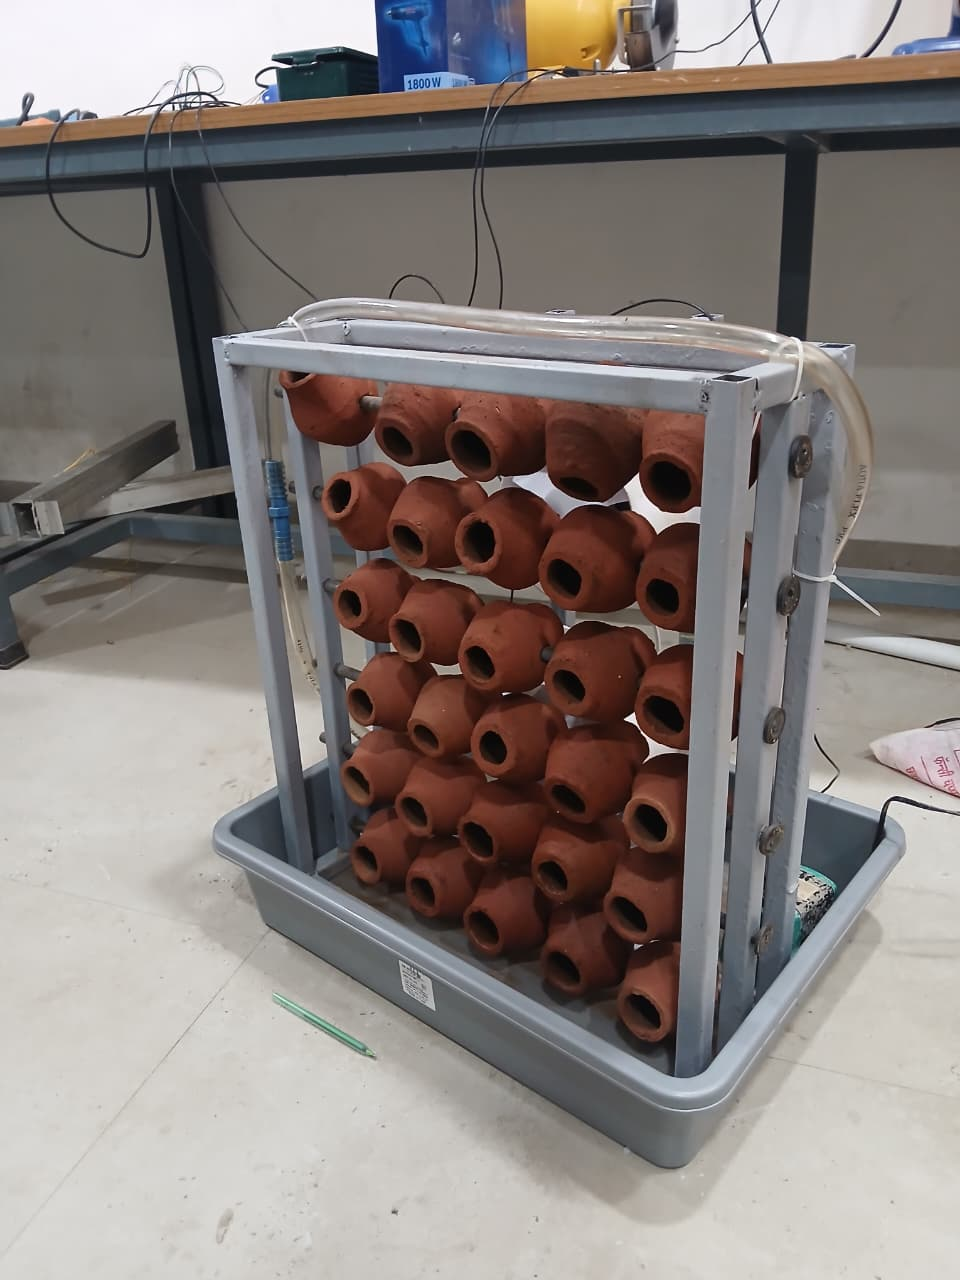
\includegraphics[height=54mm]{Water_System_Tub_Front_Right_View.jpeg} &
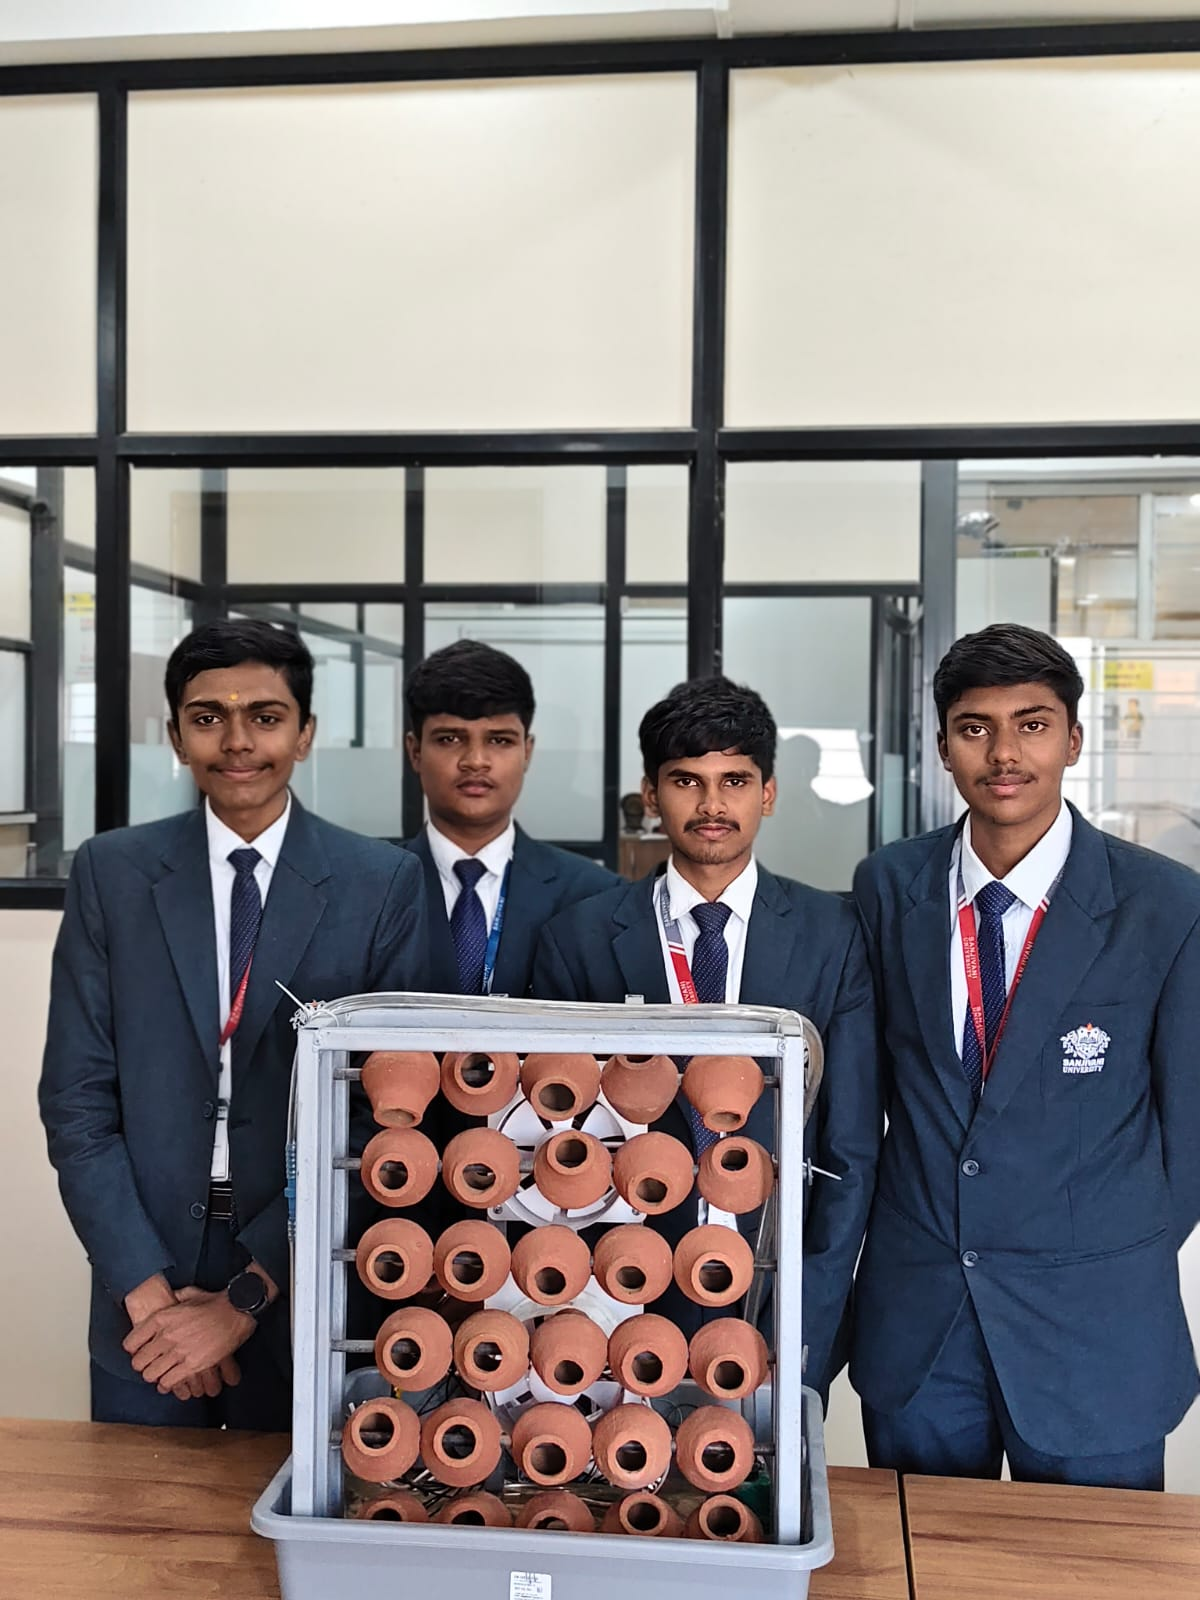
\includegraphics[height=54mm]{Team_With_Prototype.jpeg} \\[1mm]
{\footnotesize The ClayBreeze prototype} & {\footnotesize Group 17 with the ClayBreeze prototype}
\end{tabular}\par
\vspace{8mm}

{\large\textbf{Group 17}\par}
\vspace{3mm}
\begin{tabular}{l}
Tanmay Nilesh Pendbhaje \textit{(Team Leader)}\\
Harshal Kotame\\
Vedant Khairnar\\
Tanmay Mhaske\\
\end{tabular}
\vspace{8mm}

{\large Project Guide: \textbf{Dr.\ Kiran Wakchaure}\par}
\vfill
{\normalsize November 2026\par}
\end{titlepage}

% ======================= ABSTRACT =======================
\begin{abstract}
\noindent Summer heat in Indian homes, classrooms and workshops is a real and growing problem, and affordable cooling is limited: the Government of India's \emph{India Cooling Action Plan} notes that India has one of the lowest levels of access to cooling in the world~\cite{icap}. Air conditioners are expensive to buy and run and use refrigerants with climate impact; evaporative coolers are cheaper but depend on honeycomb, cellulose or grass pads that clog, degrade, can harbour mould and must be replaced.

\medskip\noindent ClayBreeze is a Makerspace prototype that replaces the consumable pad with \textbf{30 porous, unglazed terracotta pots} --- a natural, locally made, reusable and biodegradable material --- held in a welded 20\,mm square-pipe frame (480 $\times$ 560 $\times$ 150\,mm). A pump in a tub below the frame recirculates water through tubing to the top of the pots, and two rear-mounted exhaust fans blow room air through and around the wet pots. An ESP32 microcontroller reads a DHT11 temperature and humidity sensor and switches the fans and pump through a three-channel relay: both fans are off at or below 28\degC, one fan runs above 28\degC, both run above 35\degC, and the pump runs only while relative humidity is below 60\,\%.

\medskip\noindent The prototype is fully built and its control logic is running. This report documents the problem, background, design and CAD, materials, fabrication, water system, electronics, safety and the planned tests. \textbf{No performance results are reported}: low cost, low power, no pad replacement and an eco-friendly build are the design aims, and they will be checked by the measurements described in Chapter~\ref{ch:testing}.
\end{abstract}

\tableofcontents
\listoffigures
\clearpage

% ======================= 1 INTRODUCTION =======================
\chapter{Introduction and Problem}

\section{Summer heat and access to cooling}
Summers in much of India are hot, and many homes, government-school classrooms and small workshops have little or no mechanical cooling. The \emph{India Cooling Action Plan} (Ministry of Environment, Forest \& Climate Change, 2019) states that India has one of the lowest levels of access to cooling in the world, and that cooling demand --- and with it refrigerant use and energy use for cooling --- is set to rise~\cite{icap}. The plan also emphasises passive and low-energy cooling strategies alongside efficient active equipment~\cite{icap}. Practical, affordable and low-energy cooling for ordinary buildings is therefore a real engineering need, not a theoretical one.

\section{What households, schools and workshops can use today}
Table~\ref{tab:options} summarises the options we examined during a summer internship at Tinkerers' Lab, Sanjivani University. Pad-type evaporative coolers \emph{do} cool, particularly in dry air~\cite{watson}; the problems we focus on are their consumable pads, upkeep and hygiene.

\begin{table}[H]
\centering
\caption{Cooling options and their practical limitations (qualitative).}
\label{tab:options}
\small
\begin{tabularx}{\linewidth}{@{}>{\raggedright\arraybackslash}p{3.2cm}>{\raggedright\arraybackslash}X>{\raggedright\arraybackslash}X@{}}
\toprule
\textbf{Option} & \textbf{Strengths} & \textbf{Limitations} \\
\midrule
Air conditioner (vapour compression) & Controlled cooling over a wide humidity range; dehumidifies. & High purchase and running cost; high electrical demand; refrigerants with climate impact~\cite{epa,energystar,icap}. Out of reach for many households and schools. \\
Honeycomb / cellulose pad cooler & Cheaper; large wetted area; established designs. & Pads clog with scale and dust, degrade and need periodic replacement; mineral deposits reduce performance~\cite{watson,doe}; plastic bodies. \\
Grass (khus / wood-wool) pad cooler & Local, low-cost pad media; simple construction. & Damp organic pads can harbour mould and bacteria, cause odour and attract insects; combustible when dry; natural fibres degrade and need frequent replacement~\cite{alsulaiman,jain}. \\
\textbf{ClayBreeze} (this work) & Terracotta pots: natural, locally made, reusable, biodegradable; no pad to replace; ESP32 runs loads only when needed. & Design aims only --- cooling, water use, power and service life are still to be measured. \\
\bottomrule
\end{tabularx}
\end{table}

\section{Problem statement}
\begin{quote}
Summer heat in Indian homes, classrooms and workshops is a real problem, and affordable cooling is limited. Air conditioners are expensive to buy and run, draw high power and use refrigerants with climate impact. Pad-type coolers need their honeycomb or cellulose pads replaced as they clog with scale and dust, and grass pads can grow mould and bacteria, smell, attract insects, become a fire risk when dry and need frequent replacement.

\textbf{Can a low-cost, low-power cooler that uses porous, unglazed terracotta pots --- with recirculating water and automatic fan and pump control --- replace the consumable pad and produce a measurable reduction in air temperature under defined conditions?}
\end{quote}
The project must also establish whether the pots wet consistently, whether excess water returns safely to the tub, whether the frame stays stable when loaded and wet, and whether the system can be operated and maintained safely.

\section{Proposed solution}
ClayBreeze replaces the pad with 30 porous, unglazed terracotta pots arranged 5 columns $\times$ 6 rows on six \dia12\,mm rods in a welded frame. A pump in a tub under the frame lifts water through tubing to the top of the pots; excess water drains back to the tub. Two exhaust fans on a rear extension frame blow room air forward through and around the wet pots and out of the front. An ESP32 with a DHT11 sensor and a three-channel relay stages the fans by temperature and runs the pump by humidity (Chapter~\ref{ch:electronics}). The design aims are:
\begin{itemize}
\item \textbf{Low cost:} common materials --- square pipe, rods, clay pots, a plastic tub, a small pump and two fans.
\item \textbf{Low power:} two fans and a small pump, switched on only when the readings call for them.
\item \textbf{No pad replacement:} the fired clay pots are the wetted medium and are reusable.
\item \textbf{Eco-friendly:} terracotta is natural, locally made and biodegradable; no refrigerant is used.
\end{itemize}
These are aims, not results; they are tested by the plan in Chapter~\ref{ch:testing}.

\section{Inspiration: Project Vaayu}
ClayBreeze was inspired in part by reporting on \emph{Project Vaayu}, a separate student initiative in Delhi that used clay tea cups (kulhads), scrap wood and metal and water circulation to build cooling units for government-school classrooms~\cite{toi,afn}. Project Vaayu is \textbf{not our work}, and its reported outcomes are not evidence of how ClayBreeze performs; our measurements will be recorded independently.

% ======================= 2 BACKGROUND =======================
\chapter{Background and Literature}

\section{Direct evaporative cooling}
When water evaporates from a wet surface it absorbs latent heat from the water, the surface and the surrounding air. If air passes over a wetted medium, part of its sensible heat is converted into the latent energy of water vapour: the air's dry-bulb temperature can fall while its moisture content and relative humidity rise~\cite{watson}. The wet-bulb temperature is the theoretical lower limit for direct evaporative cooling. In dry air the gap between dry-bulb and wet-bulb temperature is larger, so the cooling potential is larger; in humid air it is smaller~\cite{watson}. Direct evaporative coolers always add moisture to the air, so outlet humidity must be measured alongside temperature.

\section{Porous clay and ceramic media}
Unglazed fired clay contains connected pores that absorb water and move it through the wall by capillary action, so the outer surface stays wet. Several studies have examined porous clay or ceramic media for evaporative cooling: a pottery-based direct evaporative cooling pad~\cite{laknizi}, a porous clay vessel under different ambient humidities~\cite{mittal}, a passive evaporative wall built from porous ceramics~\cite{hoyano} and an earth--air heat exchanger using porous clay vessels~\cite{elsaid}. These studies show that porous ceramics are a credible wetted medium, but their geometries, clay bodies and test conditions differ from ClayBreeze; \textbf{their results are not transferred to this prototype}.

\section{Pad materials and maintenance}
Comparative studies of pad materials --- including natural fibres such as khus and aspen and manufactured pads --- show that performance and degradation depend on the material, packing, airflow and water distribution~\cite{jain,alsulaiman}. Mineral deposits, dirt and biological growth obstruct airflow and require cleaning or pad replacement; evaporative coolers also consume water through evaporation and bleed-off~\cite{watson,doe}.

\section{Air conditioning considerations}
Room air conditioners use a compressor and refrigerant circuit. Their energy use depends on efficiency, sizing and climate~\cite{energystar}, and their climate impact depends on the refrigerant and on leakage; lower-global-warming-potential refrigerants are being adopted~\cite{epa,icap}. A fair comparison with ClayBreeze would need measured cooling, comfort and energy data, which this report does not claim.

% ======================= 3 OBJECTIVES =======================
\chapter{Objectives and Scope}

\section{Objectives}
\begin{enumerate}
\item Design and build a clay-pot evaporative cooler from natural, locally available and reusable materials, with a stable frame, secured pot-retaining rods and rear-mounted fans. \textcolor{cbok}{\textbf{Complete.}}
\item Build a recirculating water system --- tub, pump and tubing --- that wets the pots without a consumable pad. \textcolor{cbok}{\textbf{Installed}} (specifications and leak check to record).
\item Add smart, low-power control: ESP32 + DHT11 + relay, staging the fans by temperature and running the pump only below 60\,\% RH. \textcolor{cbok}{\textbf{Implemented and running.}}
\item Update the SolidWorks model and drawing to match the as-built assembly. \emph{To do.}
\item Observe whether the pots wet consistently and stay securely supported in operation. \emph{To do.}
\item Measure inlet and outlet temperature and RH, airflow, water use and electrical input against a dry-pot (fan-only) baseline. \emph{To do.}
\item Evaluate cost, maintenance and safety from measurements and records before drawing conclusions about affordability or sustainability. \emph{To do.}
\item Document design changes, trials and limitations so the work is reproducible.
\end{enumerate}

\section{Scope and limitations}
\textbf{In scope:} frame, rods and fan mounting; the water circuit; the control electronics; CAD updates from as-built measurements; controlled prototype tests where instruments are available; basic assessment of operation, cleaning and safety.

\noindent\textbf{Out of scope / not claimed:} replacing an air conditioner or a commercial cooler; any guaranteed temperature reduction, energy saving, payback or carbon reduction; whole-room comfort assessment; long-term durability and hygiene, which need extended use.

% ======================= 4 DESIGN AND CAD =======================
\chapter{Design and CAD}

\section{Design dimensions}
The frame was designed in SolidWorks. Table~\ref{tab:dims} lists the design dimensions from the dimensioned drawing (Figure~\ref{fig:drawing}). As-built dimensions have not yet been measured; the CAD model is to be revised once they are.

\begin{table}[H]
\centering
\caption{Design dimensions (SolidWorks drawing and model).}
\label{tab:dims}
\small
\begin{tabular}{@{}ll@{}}
\toprule
\textbf{Parameter} & \textbf{Value} \\
\midrule
Frame outer size (W $\times$ H $\times$ D) & 480 $\times$ 560 $\times$ 150\,mm \\
Front opening & 440 $\times$ 520\,mm \\
Frame section & 20\,mm square pipe (wall thickness to be confirmed) \\
Overall depth with rear fan-mount extension & 270\,mm \\
Pot-retaining rods & 6 $\times$ \dia12\,mm, 90\,mm pitch (CAD) \\
Pot array & 30 pots, 5 columns $\times$ 6 rows \\
Pot model size (CAD) & \dia80\,mm max, 80\,mm long, \dia40\,mm openings \\
Fan-mount members & centred 132.5\,mm in from each side member \\
\bottomrule
\end{tabular}
\end{table}

\begin{figure}[H]
\centering
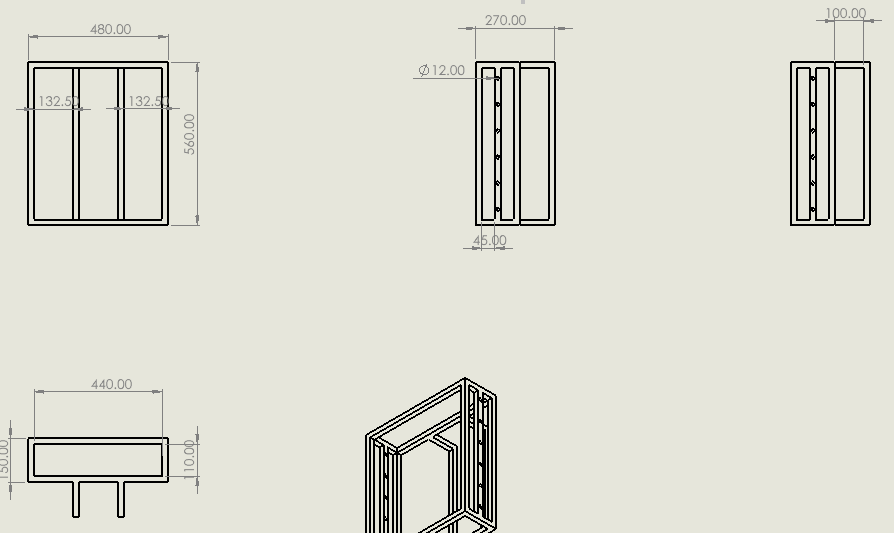
\includegraphics[width=0.95\linewidth]{cad-drawing-full.png}
\caption{SolidWorks engineering drawing of the frame (cropped from the drawing sheet): front view (480 $\times$ 560\,mm), side view (270\,mm overall depth, \dia12\,mm rod), top views (440 $\times$ 150\,mm) and isometric view.}
\label{fig:drawing}
\end{figure}

\begin{figure}[H]
\centering
\begin{subfigure}[b]{0.56\linewidth}\centering
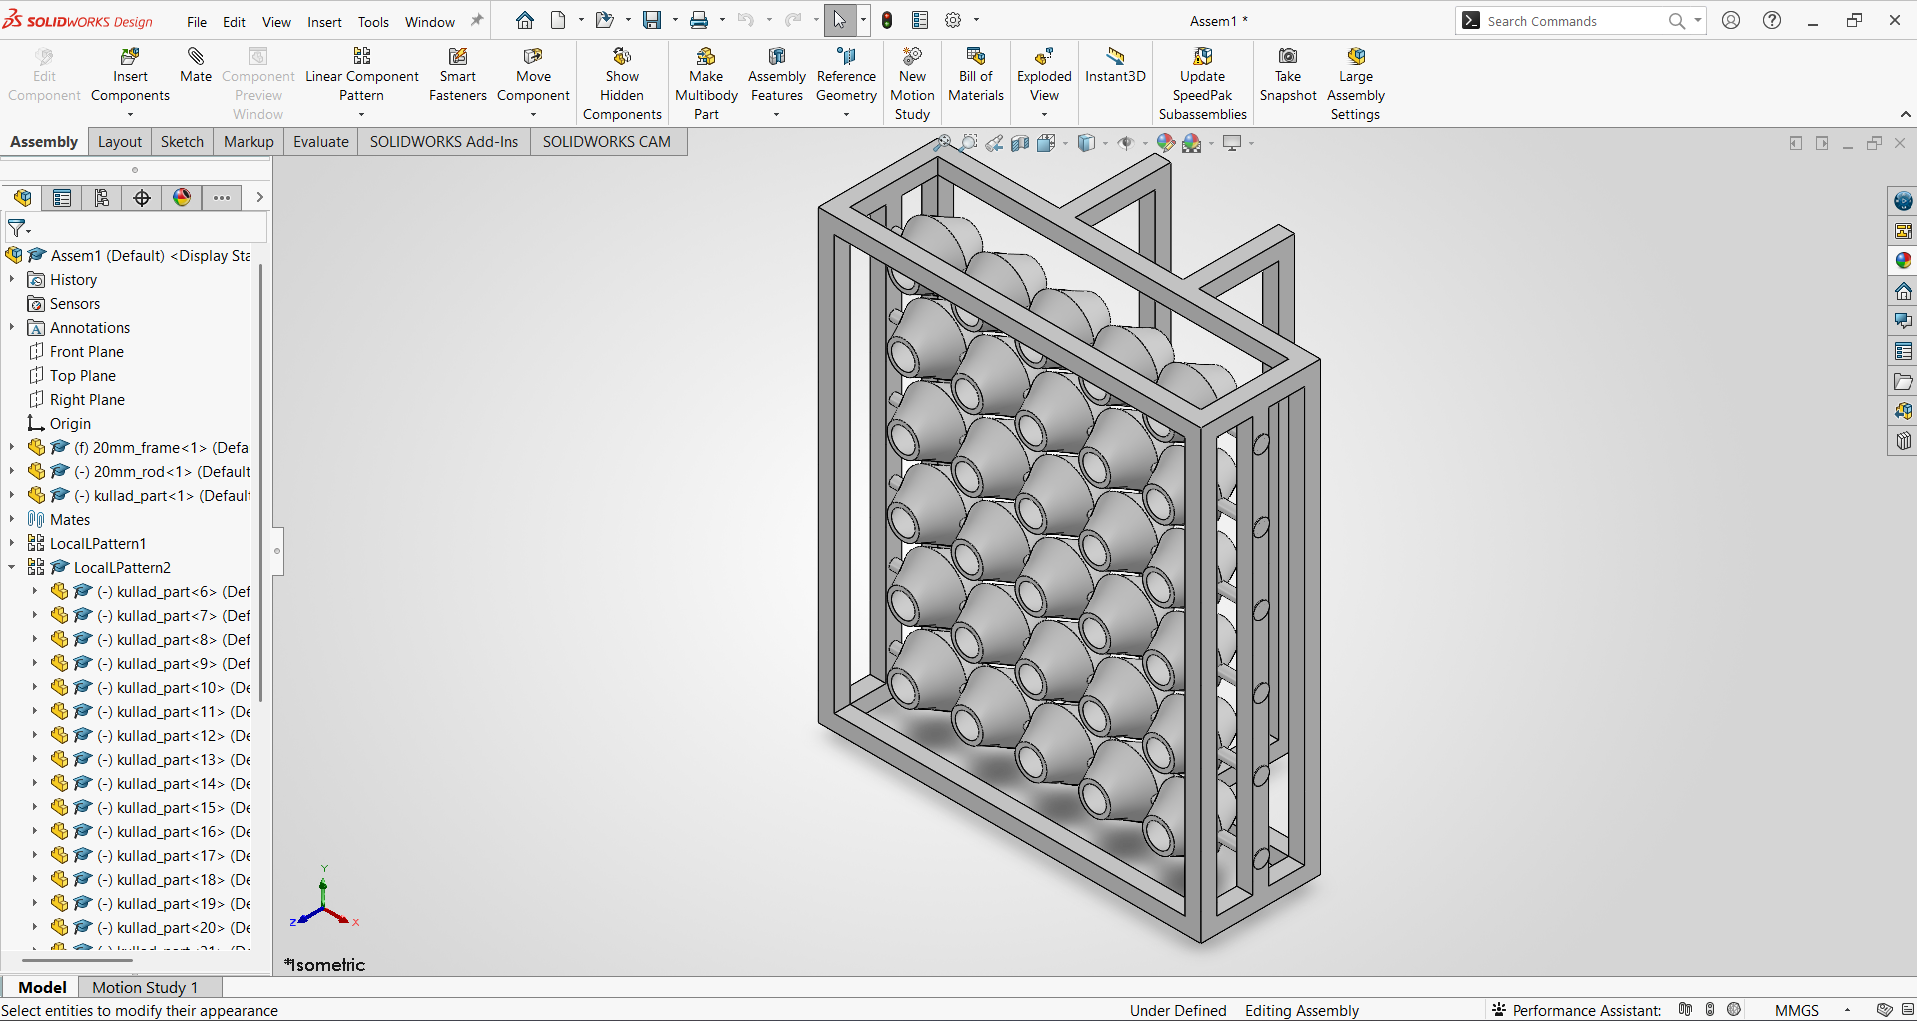
\includegraphics[width=\linewidth, trim=468 24 336 100, clip]{Assembly_Isometric_View.png}
\caption{Assembly, isometric view}
\end{subfigure}\hfill
\begin{subfigure}[b]{0.4\linewidth}\centering
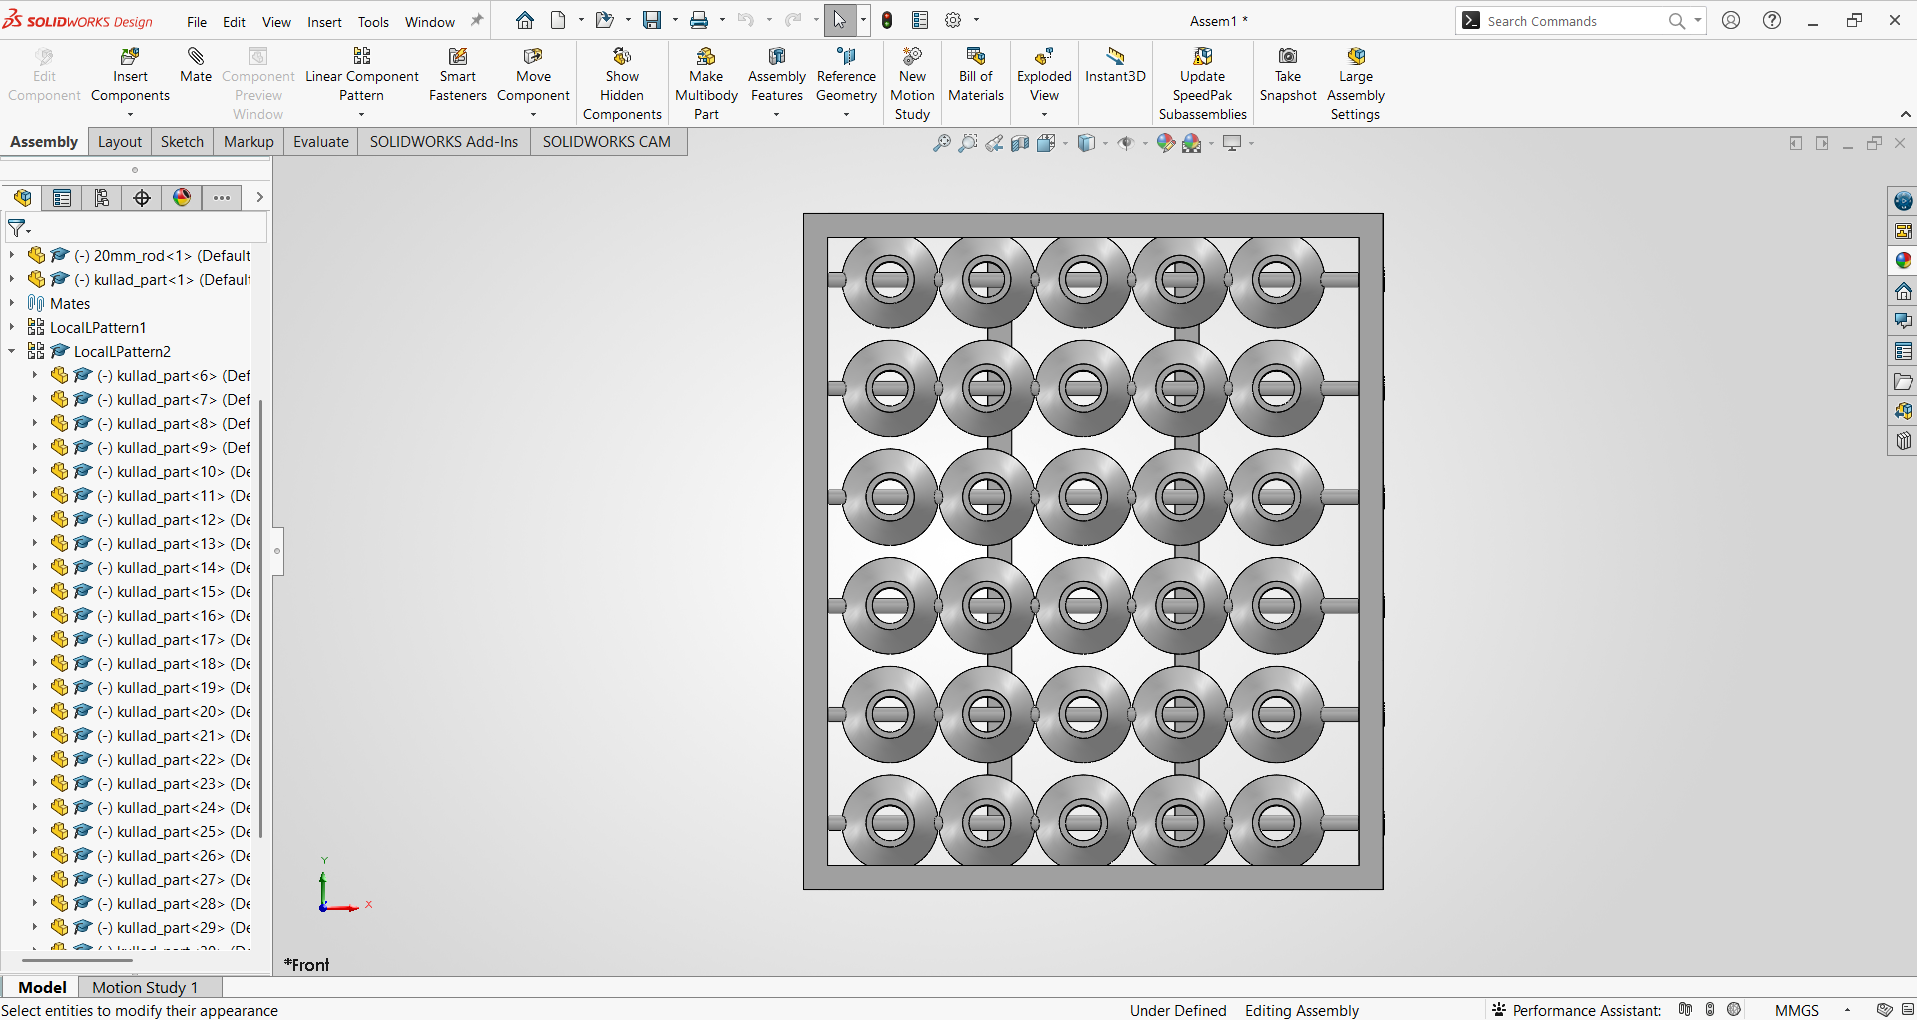
\includegraphics[width=\linewidth, trim=420 24 270 96, clip]{Assebly_Front_View.png}
\caption{Assembly, front view (5 $\times$ 6 pots)}
\end{subfigure}
\caption{SolidWorks assembly: frame, rear extension, rods and the 30-pot array.}
\label{fig:assembly}
\end{figure}

\begin{figure}[H]
\centering
\begin{subfigure}[b]{0.32\linewidth}\centering
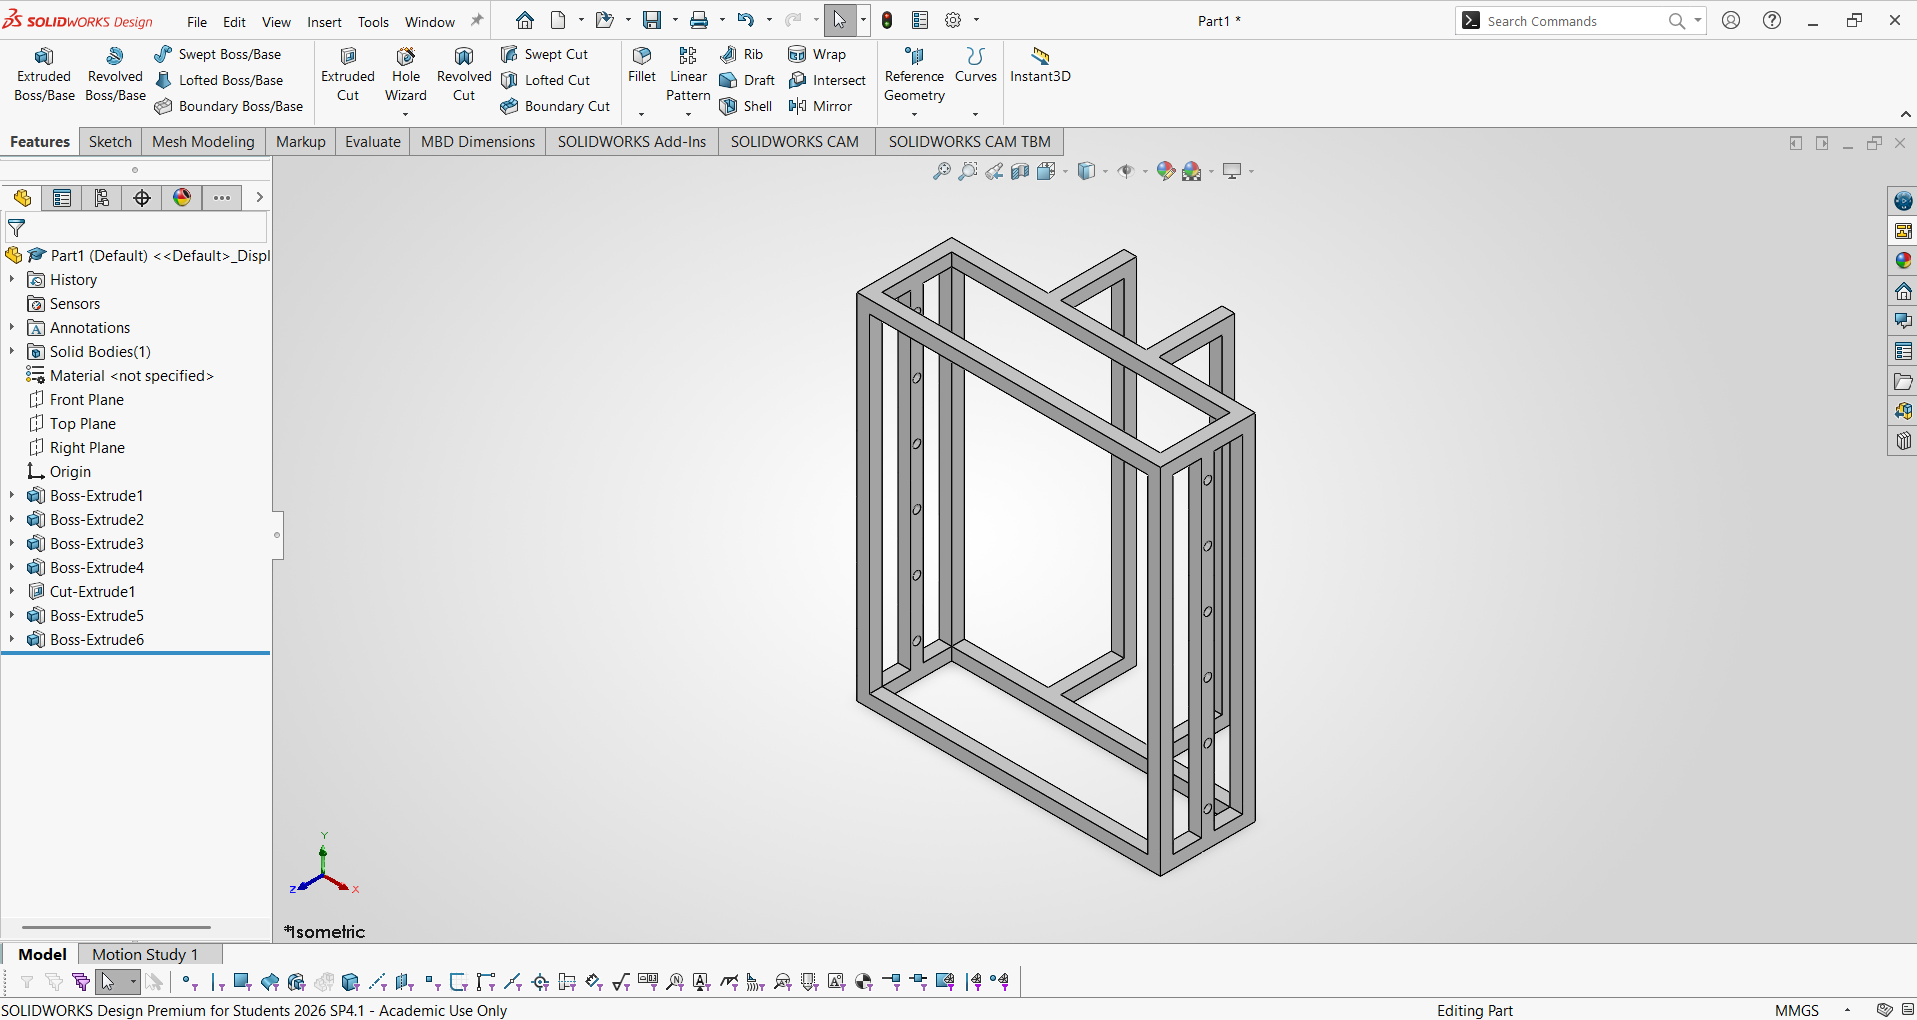
\includegraphics[width=\linewidth, trim=420 72 300 96, clip]{Frame.png}
\caption{Frame with extension}
\end{subfigure}\hfill
\begin{subfigure}[b]{0.32\linewidth}\centering
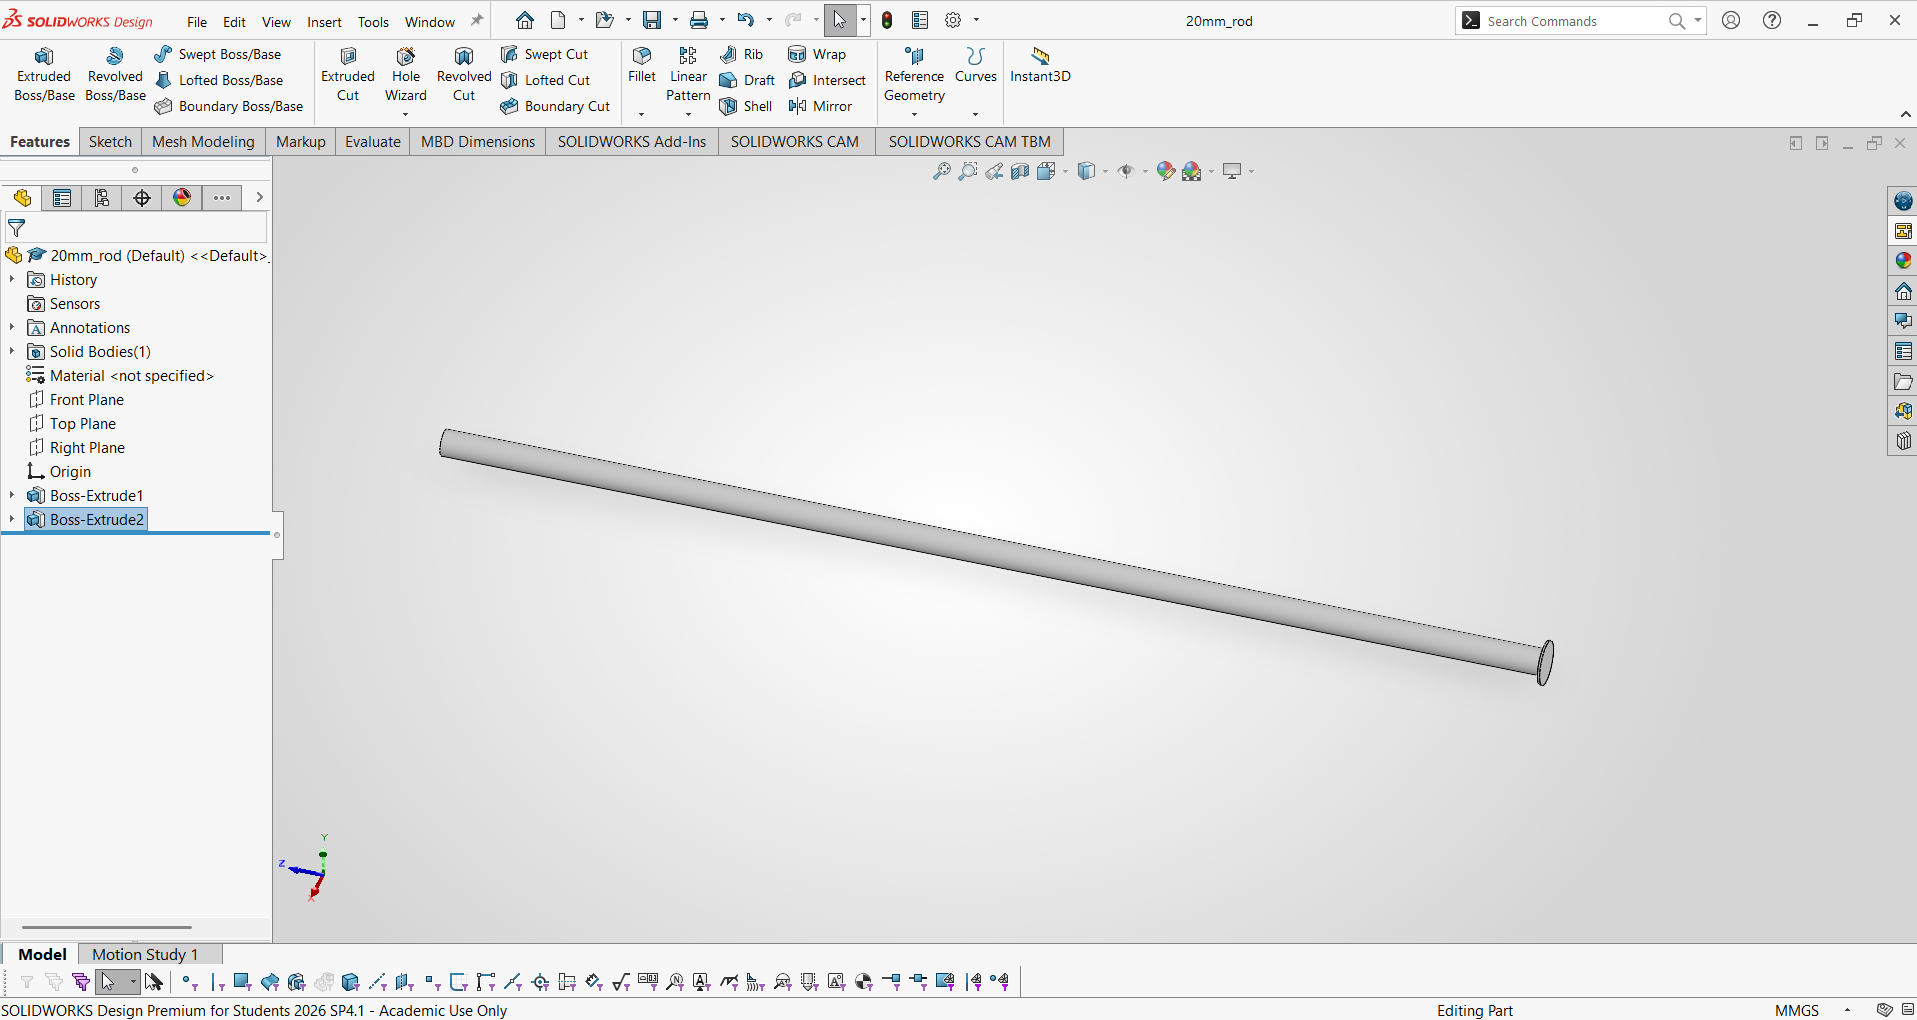
\includegraphics[width=\linewidth, trim=420 150 300 150, clip]{Rod.png}
\caption{Retaining rod}
\end{subfigure}\hfill
\begin{subfigure}[b]{0.32\linewidth}\centering
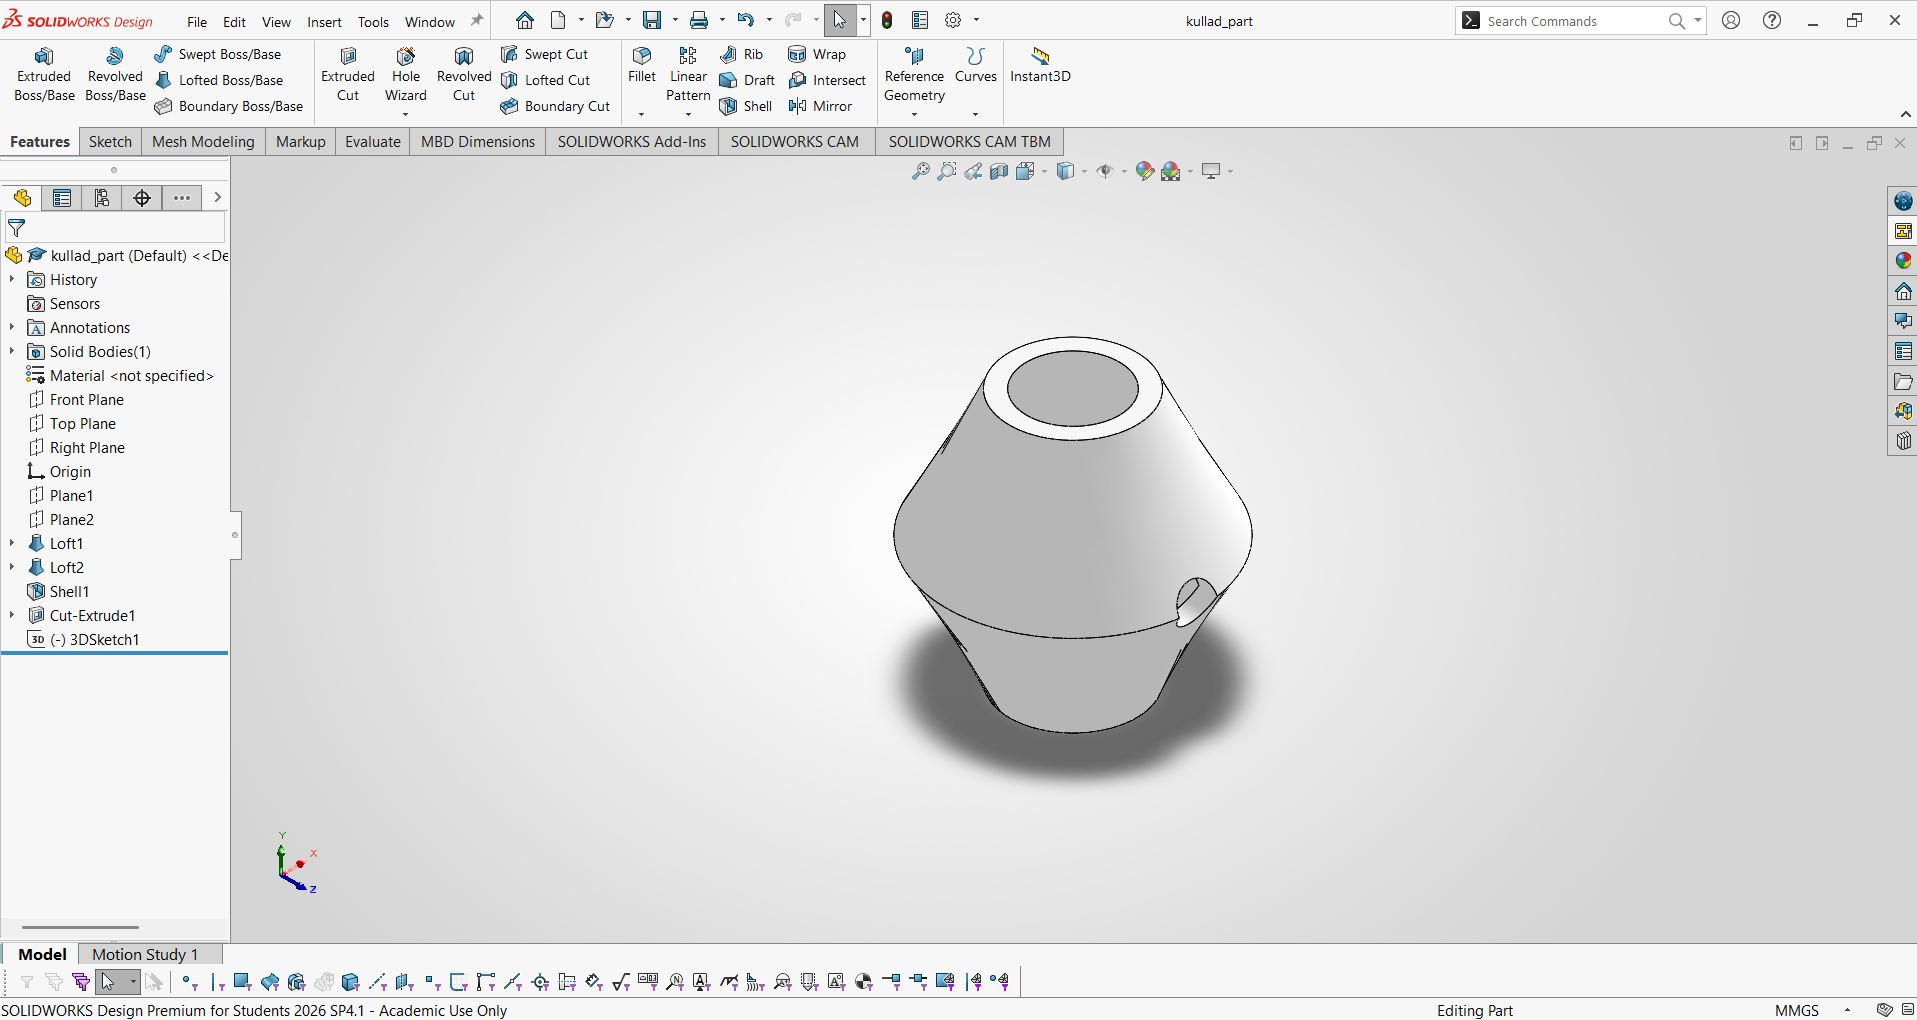
\includegraphics[width=\linewidth, trim=450 120 330 120, clip]{Clay_Pot.png}
\caption{Clay pot (kullad\_part)}
\end{subfigure}
\caption{SolidWorks part models. The rod file is named ``20mm\_rod'', but the drawing calls it out at \dia12\,mm, matching the physical rods.}
\label{fig:parts}
\end{figure}

\section{Working principle}
Figure~\ref{fig:schematic} shows the intended air and water paths. The two fans on the rear extension take in room air from behind and blow it forward through and around the pots and out of the front. Water goes from the tub to the pump, up the tubing to the top of the pots, and drains back to the tub. Because the pots do not seal against each other or the frame, some air bypasses them; this has not been measured.

\begin{figure}[H]
\centering
\resizebox{0.9\linewidth}{!}{% ClayBreeze working-principle schematic (side view), shared by the poster and the report.
% Conceptual — not measured. Coordinates follow the website SVG (x right, y down), 760 x 330 units.
% Use inside \resizebox{<width>}{!}{\input{.../schematic.tex}}.
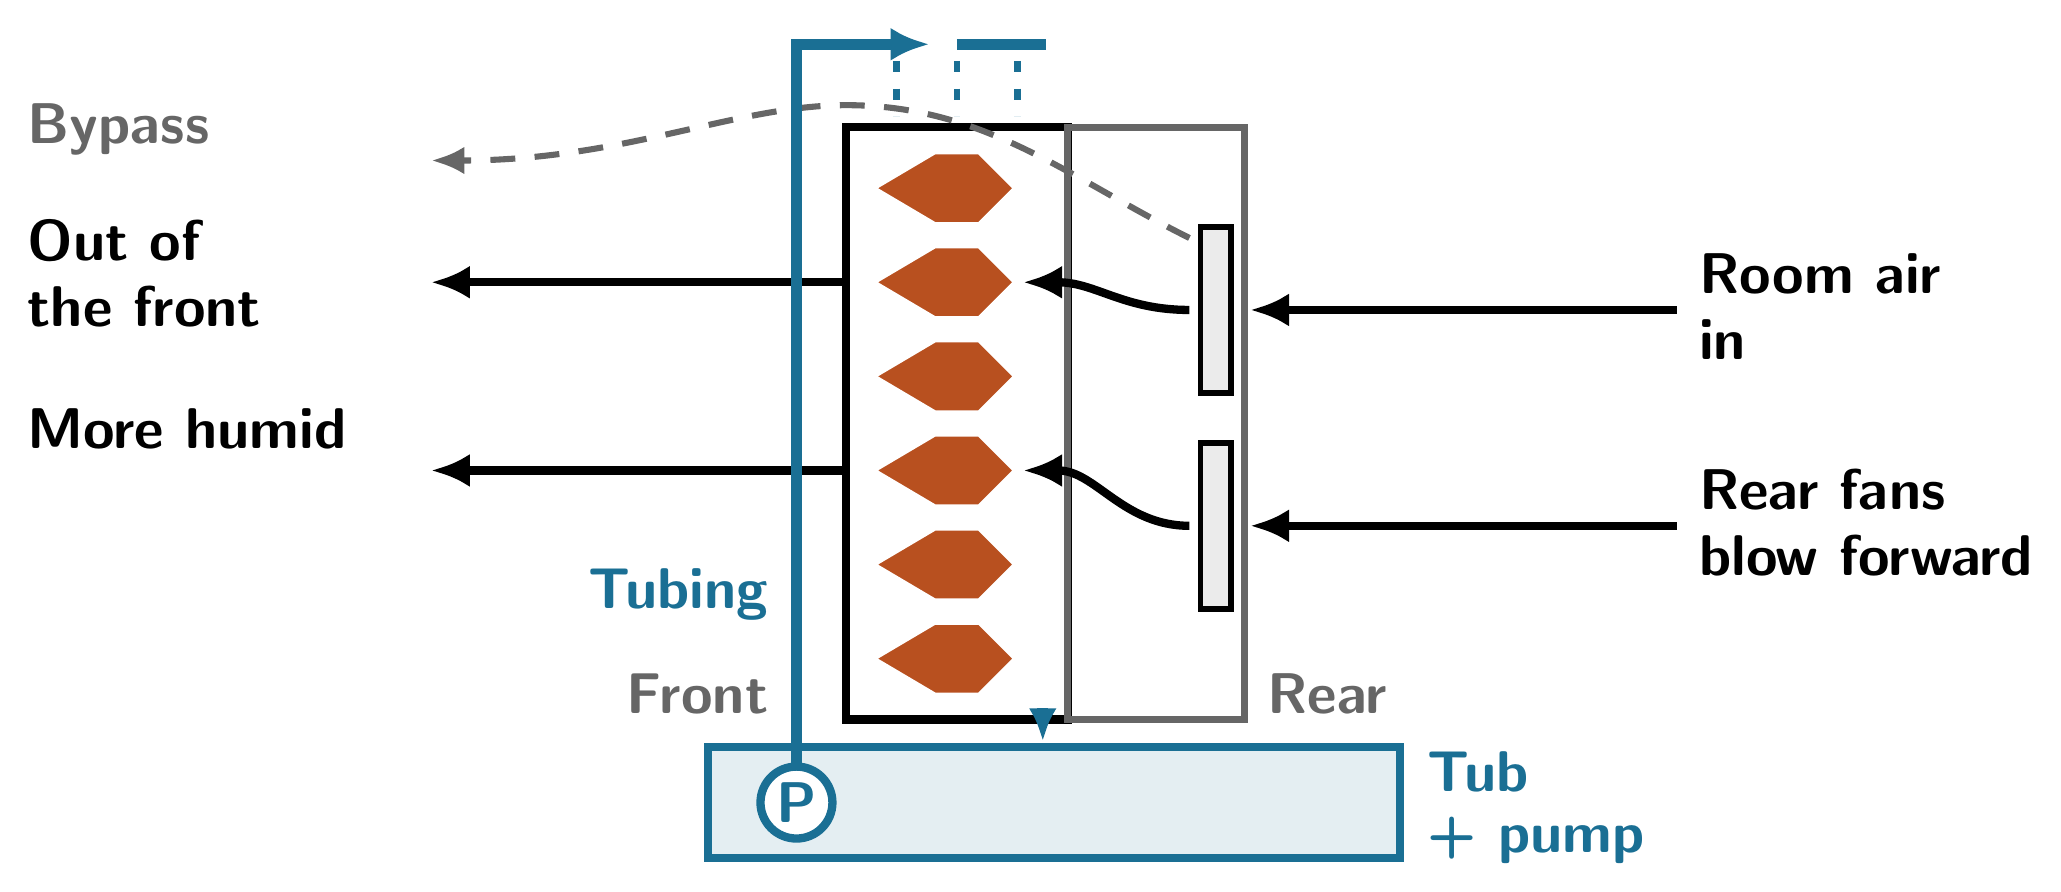
\begin{tikzpicture}[x=1pt, y=-1pt, font=\sffamily\bfseries\fontsize{21}{24}\selectfont,
    air/.style={line width=3pt, -{Latex[length=14pt,width=12pt]}, black},
    bypass/.style={line width=2.2pt, dash pattern=on 9pt off 7pt, -{Latex[length=12pt,width=10pt]}, black!60},
    water/.style={line width=4pt, cbwater},
    lbl/.style={anchor=base west, inner sep=0pt}]
  % frame (main) and rear extension
  \draw[line width=3pt] (300,52) rectangle (380,266);
  \draw[line width=2.5pt, black!60] (380,52) rectangle (444,266);
  % pots on six rods
  \foreach \y in {74,108,142,176,210,244}
    \fill[cbclay, draw=white, line width=1.5pt] (310,\y) -- (332,\y-13) -- (348,\y-13) -- (361,\y) -- (348,\y+13) -- (332,\y+13) -- cycle;
  % fans
  \draw[line width=2pt, fill=black!8] (428,88) rectangle (439,148);
  \draw[line width=2pt, fill=black!8] (428,166) rectangle (439,226);
  % air path
  \draw[air] (600,118) -- (446,118);
  \draw[air] (600,196) -- (446,196);
  \draw[air] (424,118) .. controls (400,118) and (390,108) .. (364,108);
  \draw[air] (424,196) .. controls (400,196) and (390,176) .. (364,176);
  \draw[air] (300,108) -- (150,108);
  \draw[air] (300,176) -- (150,176);
  \draw[bypass] (424,92) .. controls (380,70) and (350,44) .. (300,44) .. controls (260,44) and (220,64) .. (150,64);
  \node[lbl] at (608,112) {Room air};
  \node[lbl] at (608,136) {in};
  \node[lbl] at (608,190) {Rear fans};
  \node[lbl] at (608,214) {blow forward};
  \node[lbl] at (4,100) {Out of};
  \node[lbl] at (4,124) {the front};
  \node[lbl] at (4,168) {More humid};
  \node[lbl, black!60] at (4,58) {Bypass};
  \node[anchor=base east, inner sep=0pt, black!60] at (272,264) {Front};
  \node[lbl, black!60] at (452,264) {Rear};
  % water path: tub -> pump -> tubing -> top of pots -> back to tub
  \draw[line width=3pt, cbwater, fill=cbwater!12] (250,276) rectangle (500,316);
  \draw[line width=3pt, cbwater, fill=white] (282,296) circle (13);
  \node[cbwater] at (282,296) {P};
  \draw[water, -{Latex[length=14pt,width=12pt]}] (282,283) -- (282,22) -- (330,22);
  \draw[water] (340,22) -- (372,22);
  \foreach \x in {318,340,362} \draw[cbwater, line width=2.5pt, dash pattern=on 4pt off 6pt] (\x,28) -- (\x,48);
  \draw[water, -{Latex[length=12pt,width=10pt]}] (371,262) -- (371,274);
  \node[lbl, cbwater] at (510,292) {Tub};
  \node[lbl, cbwater] at (510,314) {+ pump};
  \node[anchor=base east, inner sep=0pt, cbwater] at (272,226) {Tubing};
\end{tikzpicture}
}
\caption{Working principle, side view (conceptual --- not measured). Air: room air $\rightarrow$ rear fans $\rightarrow$ through and around the pots $\rightarrow$ front. Water: tub $\rightarrow$ pump $\rightarrow$ tubing $\rightarrow$ pots $\rightarrow$ tub.}
\label{fig:schematic}
\end{figure}

% ======================= 5 MATERIALS =======================
\chapter{Materials and Components}

Table~\ref{tab:materials} lists the materials and components. Makes, models and ratings that have not been recorded are marked as such rather than estimated. Costs are not reported because no cost record exists yet.

\begin{table}[H]
\centering
\caption{Materials and components.}
\label{tab:materials}
\small
\begin{tabularx}{\linewidth}{@{}>{\raggedright\arraybackslash}p{3.6cm}>{\raggedright\arraybackslash}p{1.4cm}>{\raggedright\arraybackslash}X@{}}
\toprule
\textbf{Item} & \textbf{Qty} & \textbf{Notes} \\
\midrule
Square metal pipe, 20\,mm & as cut & Frame and rear fan-mount extension; welded and spray-painted grey. Wall thickness and grade to record. \\
Steel rods, \dia12\,mm & 6 & Pot-retaining rods through drilled holes in the frame. \\
Unglazed clay pots (kulhad type) & 30 & Hollow-through, 5 $\times$ 6. Size, mass and porosity to measure. \\
Exhaust fans & 2 & On the rear extension, blowing forward. Model and rating to record. \\
Plastic tub (reservoir) & 1 & Grey tub under the frame; collects return water. Size and capacity to record. \\
Water pump & 1 & In the tub; switched by the relay. Model, flow and head to record. \\
Clear tubing and connector & as fitted & From the pump up the frame to the top of the pots. Length and bore to record. \\
ESP32 development board & 1 & Runs the control logic. \\
DHT11 sensor & 1 & Temperature and relative humidity. \\
3-channel relay module & 1 & Switches fan 1, fan 2 and the pump. \\
Breadboard, jumper wires & -- & Prototype wiring; not water-resistant. \\
Spray paint, welding consumables & -- & Frame finishing and fabrication. \\
\bottomrule
\end{tabularx}
\end{table}

% ======================= 6 FABRICATION =======================
\chapter{Fabrication Process}

The prototype was fabricated in the university workshop. The steps below follow the photographs taken during the build; dates are not recorded because the photographs carry no date metadata.

\section{Cutting and welding the frame}
The 20\,mm square pipe was marked and cut to length on an abrasive chop saw, sorted by length and welded into a box frame (Figure~\ref{fig:fab1}).

\begin{figure}[H]
\centering
\begin{subfigure}[b]{0.24\linewidth}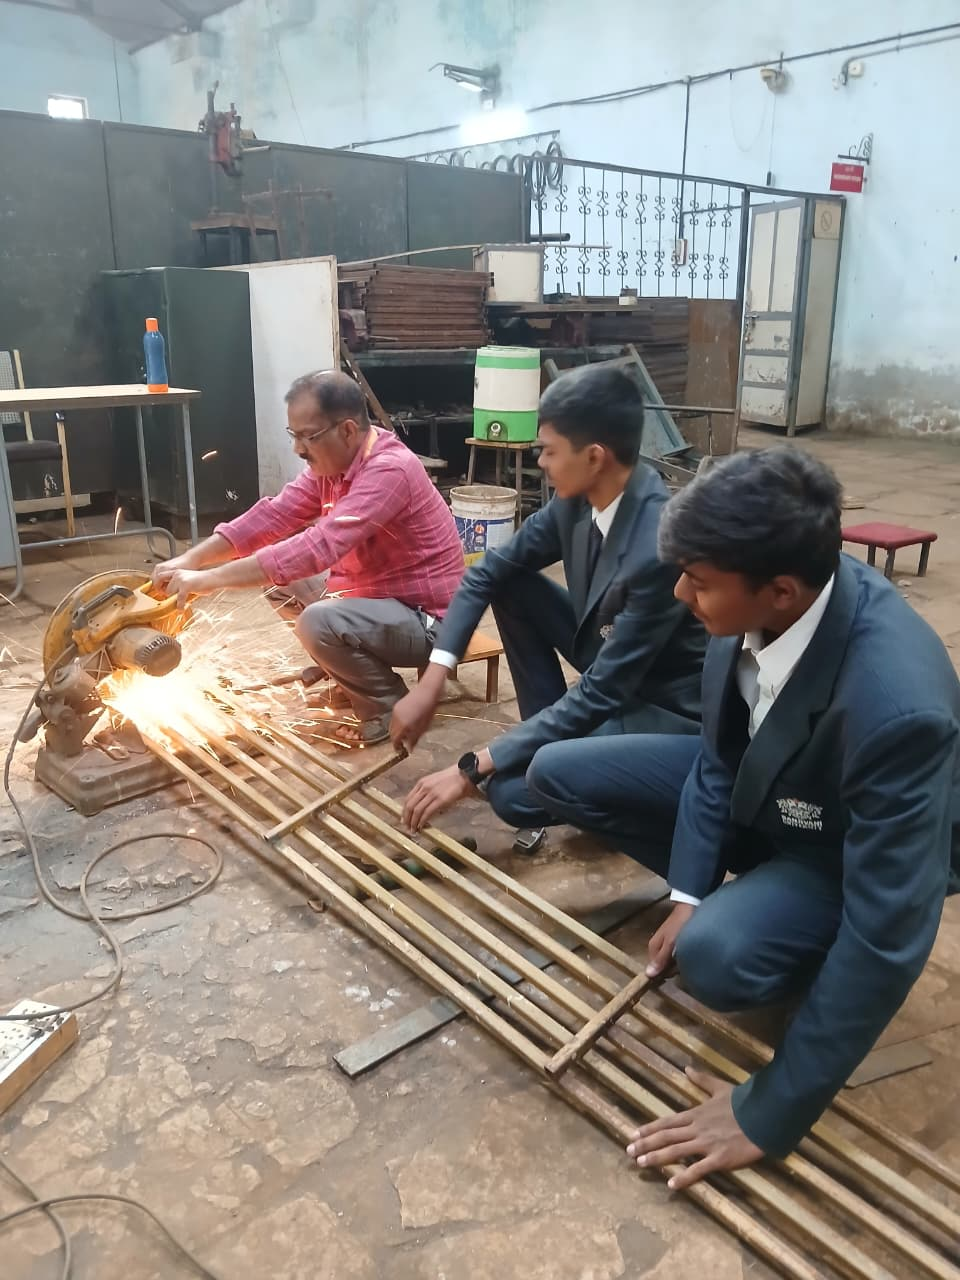
\includegraphics[width=\linewidth]{Frame_pipe_cutting_1.jpeg}\caption{Cutting pipe}\end{subfigure}\hfill
\begin{subfigure}[b]{0.24\linewidth}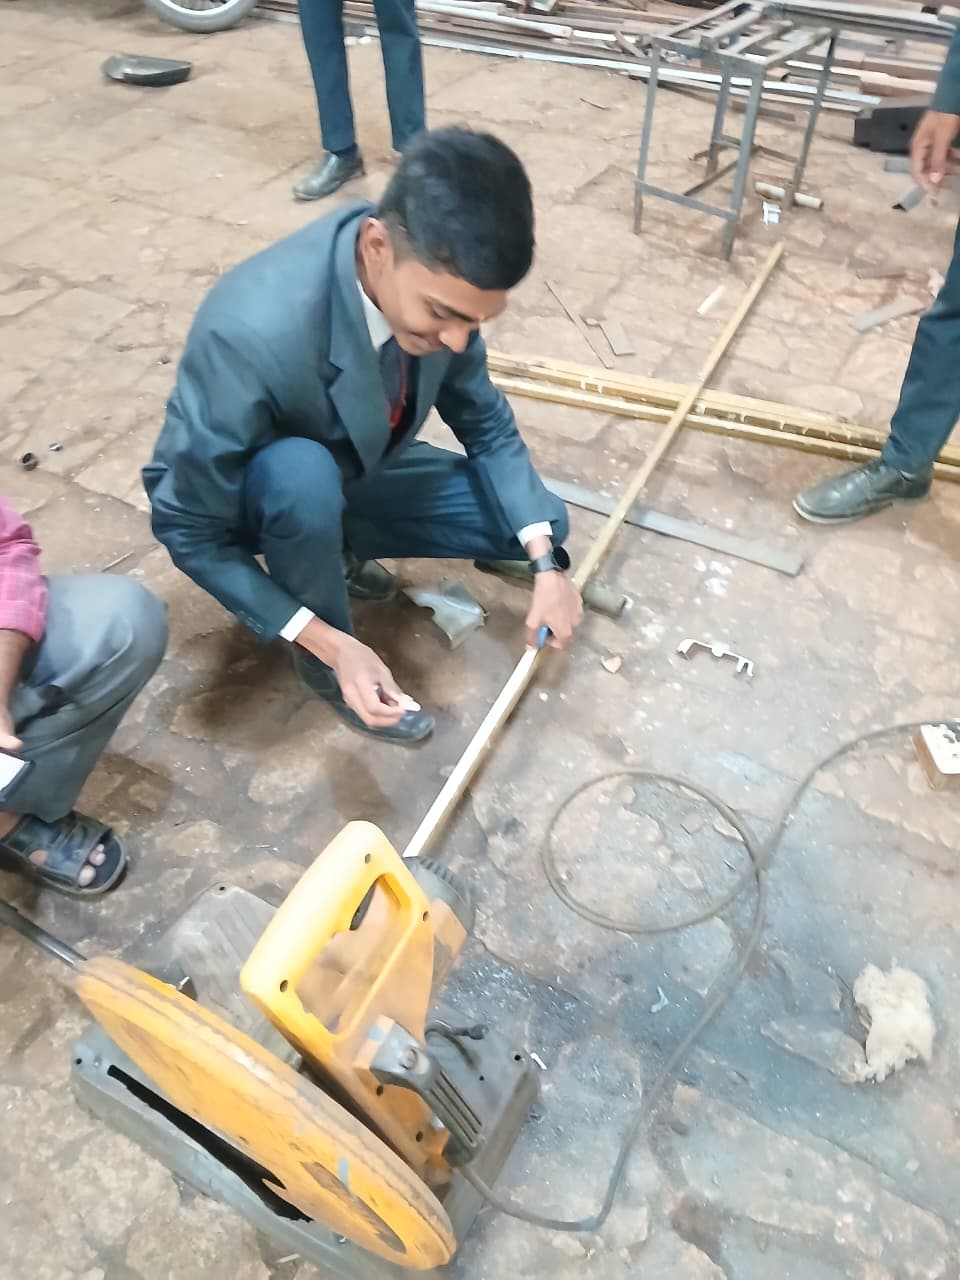
\includegraphics[width=\linewidth]{Frame_pipe_cutting_3.jpeg}\caption{Marking length}\end{subfigure}\hfill
\begin{subfigure}[b]{0.24\linewidth}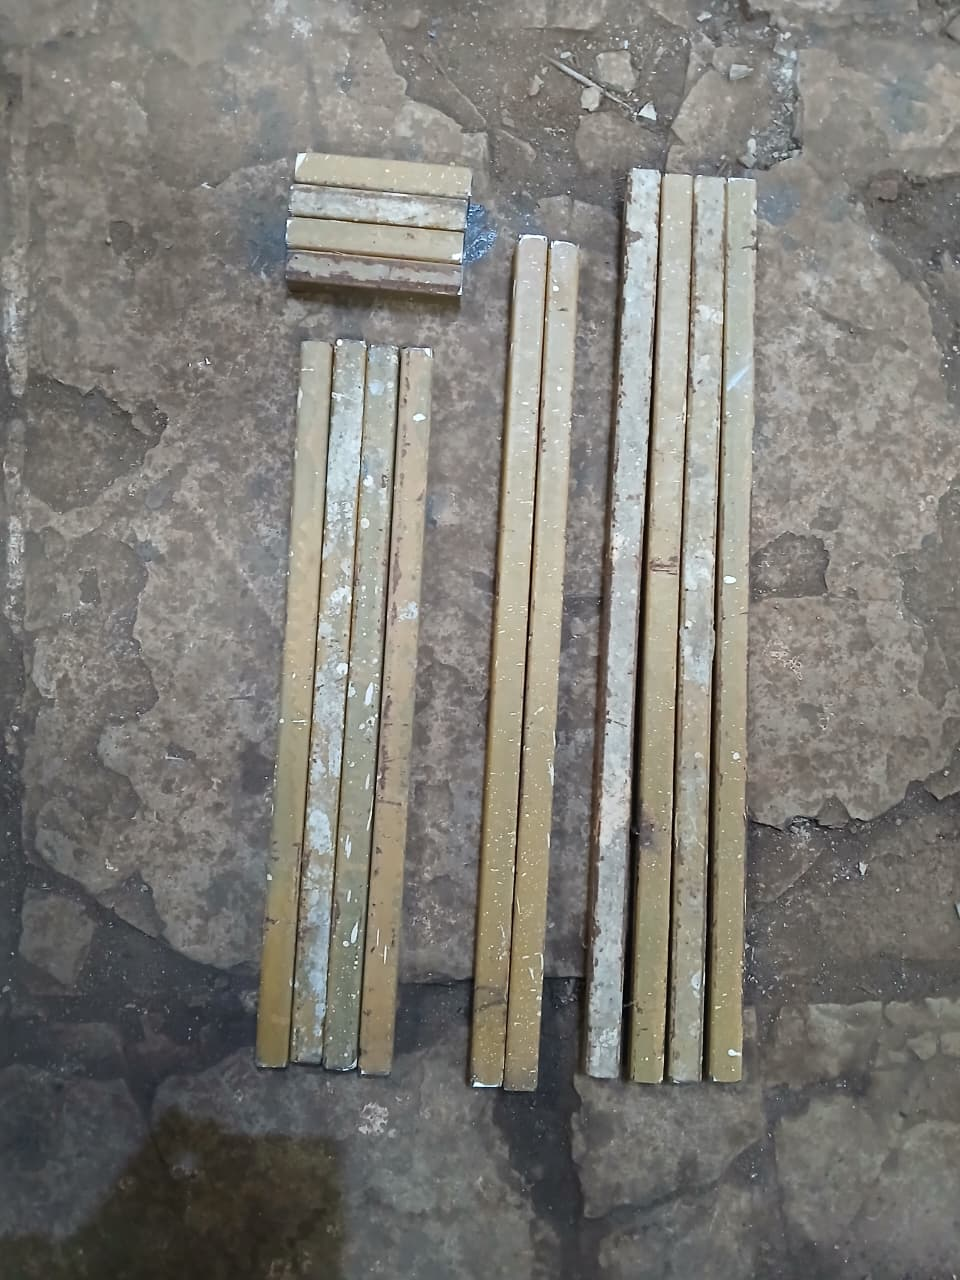
\includegraphics[width=\linewidth]{Pipes_Cut_All_1.jpeg}\caption{Cut sections}\end{subfigure}\hfill
\begin{subfigure}[b]{0.24\linewidth}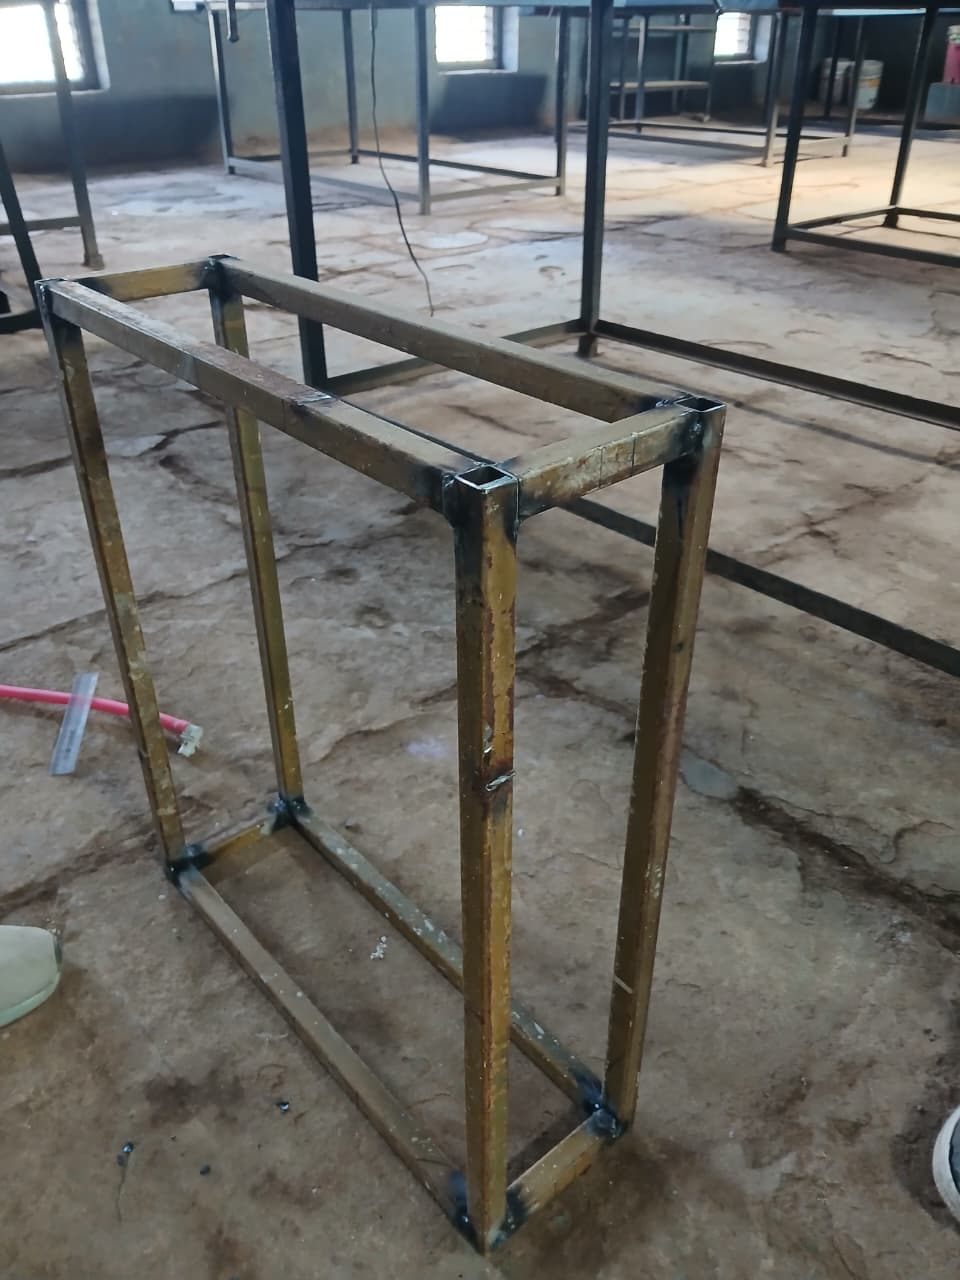
\includegraphics[width=\linewidth]{Frame_Welded_1.jpeg}\caption{Welded frame}\end{subfigure}
\caption{Cutting and welding the square-pipe frame.}
\label{fig:fab1}
\end{figure}

\section{Marking and drilling the rod holes; fitting the rods}
Rod-hole positions were centre-punched on the square-pipe members so the drill would start accurately. The holes were drilled and six \dia12\,mm rods were fitted across the width of the frame. A rear extension frame was then welded on to carry the fans (Figure~\ref{fig:fab2}).

\begin{figure}[H]
\centering
\begin{subfigure}[b]{0.3\linewidth}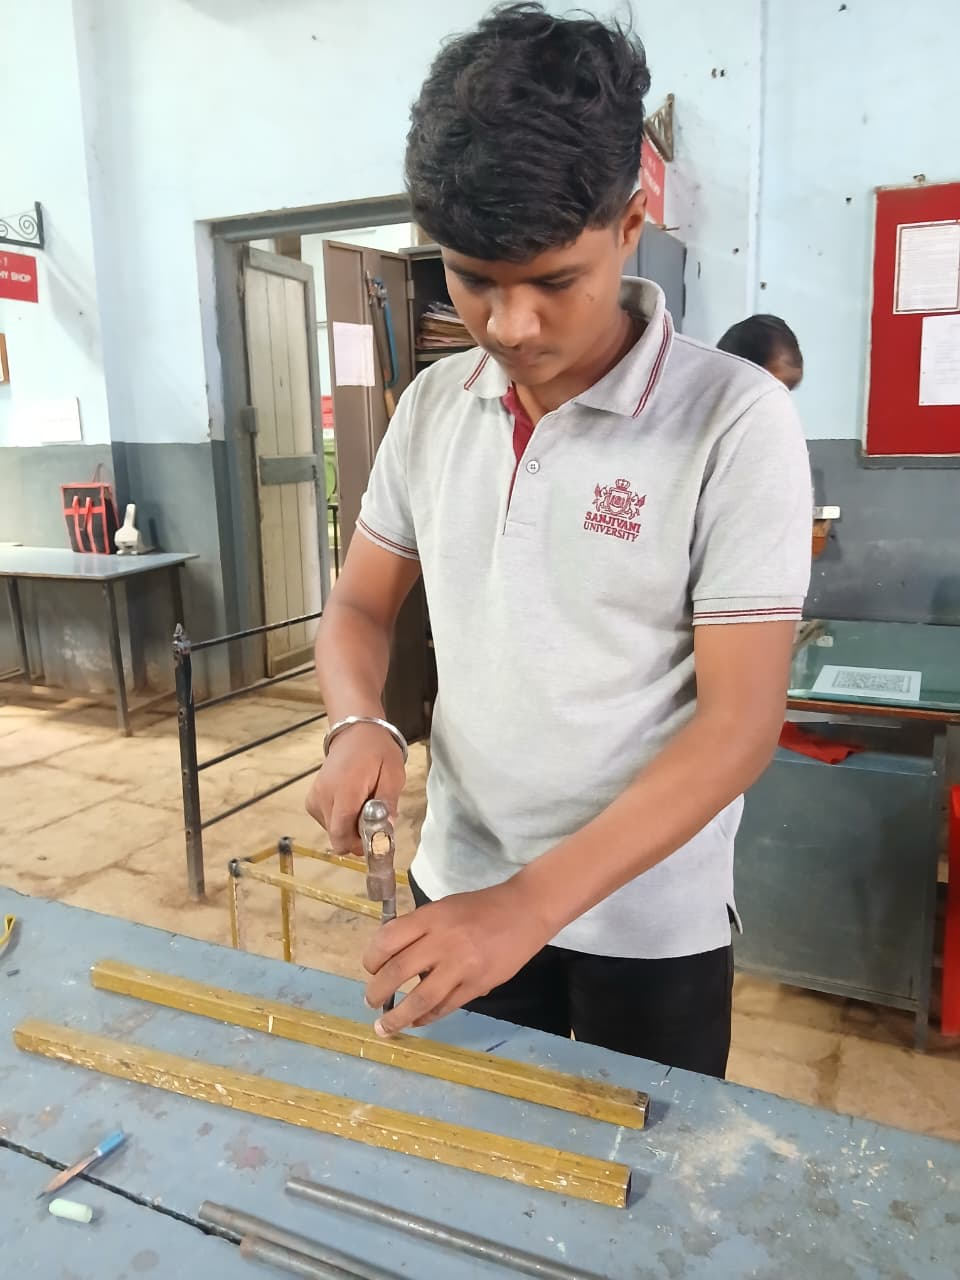
\includegraphics[width=\linewidth, trim=0 0 0 0]{Drill_Point_Marking_2.jpeg}\caption{Centre-punching}\end{subfigure}\hfill
\begin{subfigure}[b]{0.3\linewidth}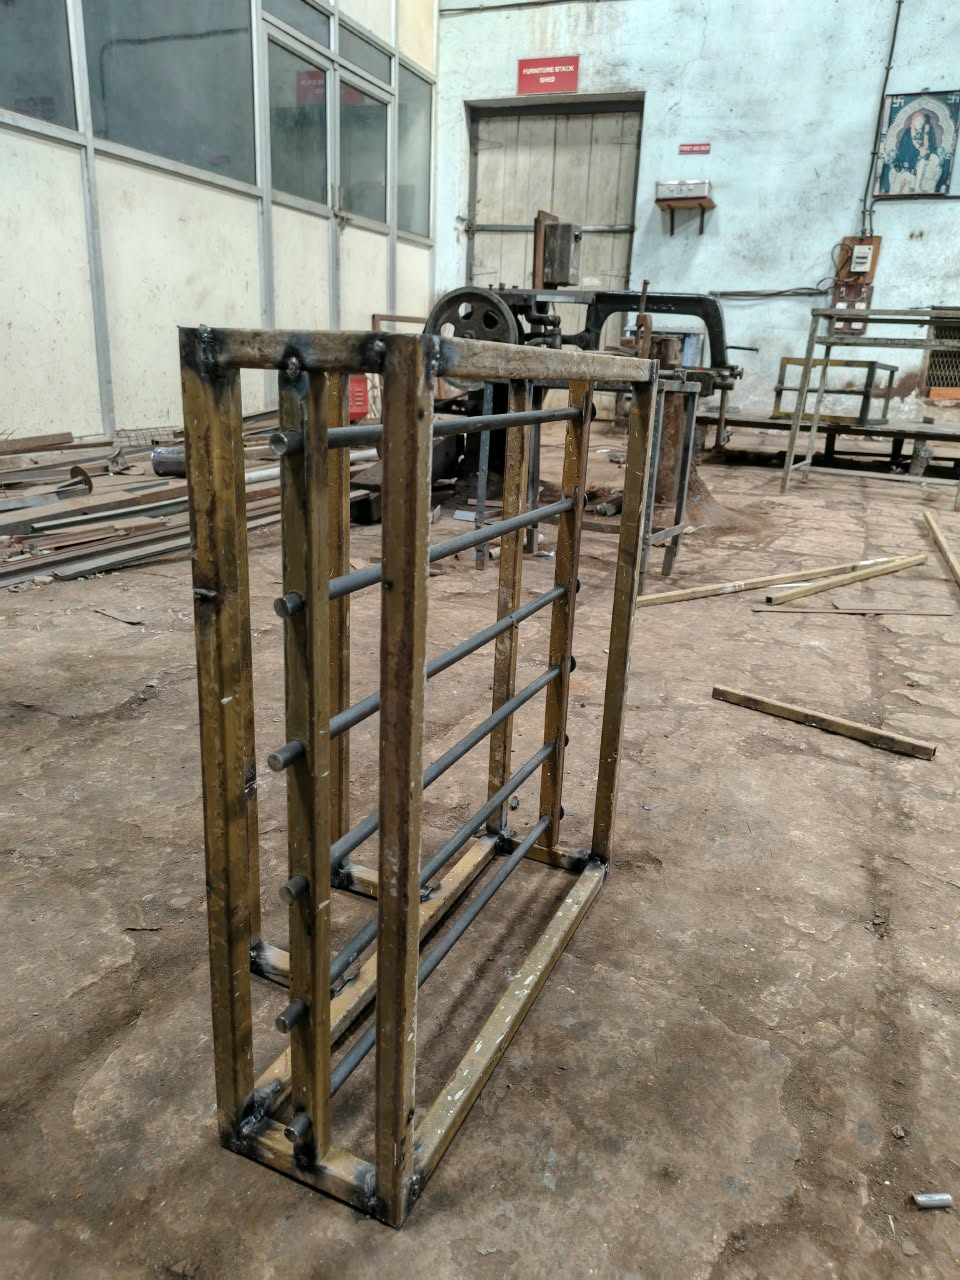
\includegraphics[width=\linewidth]{Frame_Rod_Assembled_1.jpeg}\caption{Rods fitted}\end{subfigure}\hfill
\begin{subfigure}[b]{0.3\linewidth}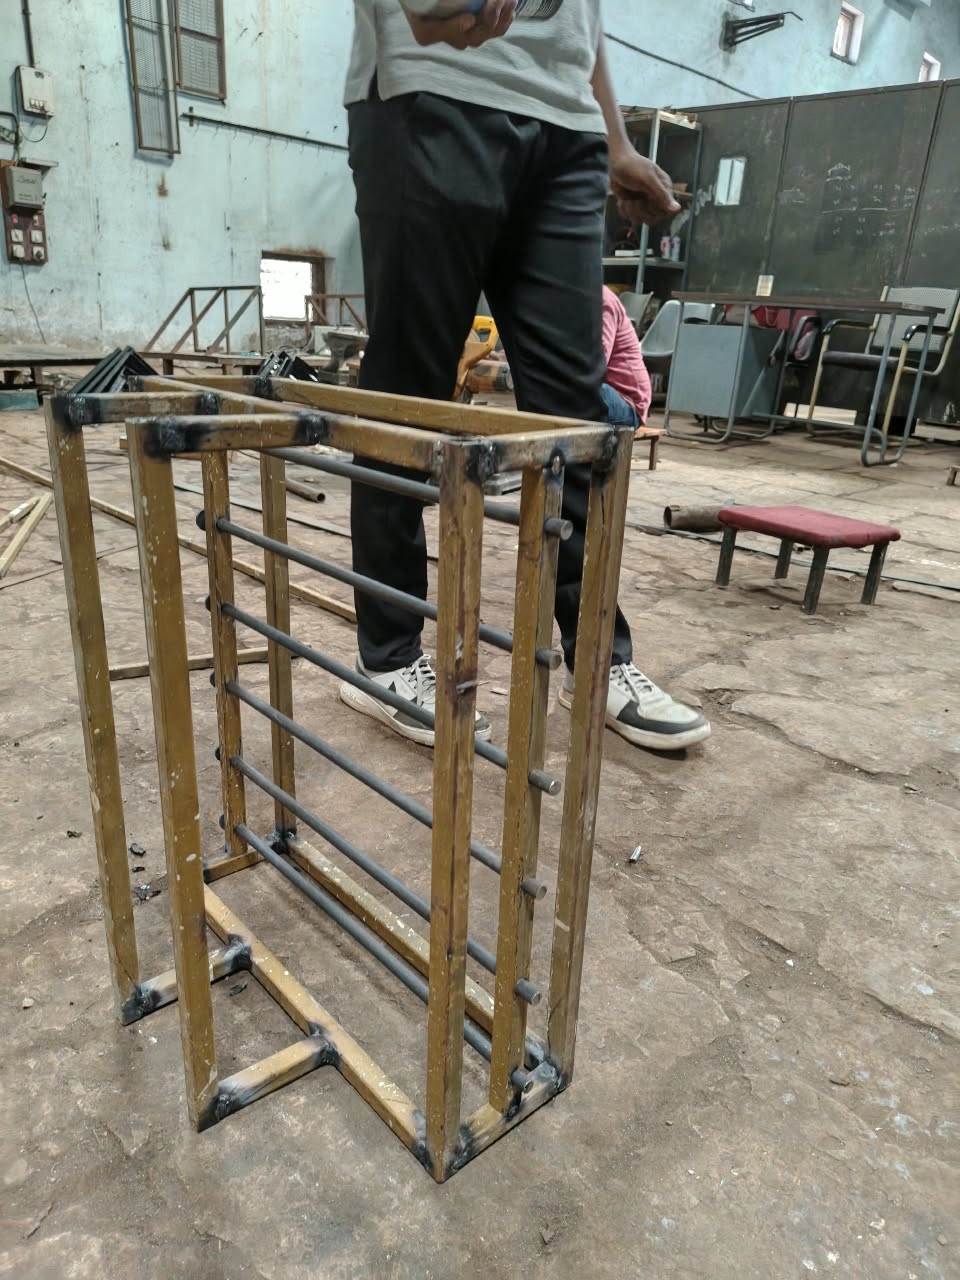
\includegraphics[width=\linewidth]{Frame_Rod_assembled_With_Fan_Extension1.jpeg}\caption{Rear fan-mount extension}\end{subfigure}
\caption{Rod holes, rods and the rear fan-mount extension.}
\label{fig:fab2}
\end{figure}

\section{Painting, fans and pots}
The frame was spray-painted grey and the two exhaust fans were mounted one above the other on the rear extension, facing forward. Thirty unglazed clay pots were then threaded onto the rods, mouths facing the front (Figure~\ref{fig:fab3}). The photographs show a loose fan cable at the top of the frame, which must be secured before powered testing.

\begin{figure}[H]
\centering
\begin{subfigure}[b]{0.3\linewidth}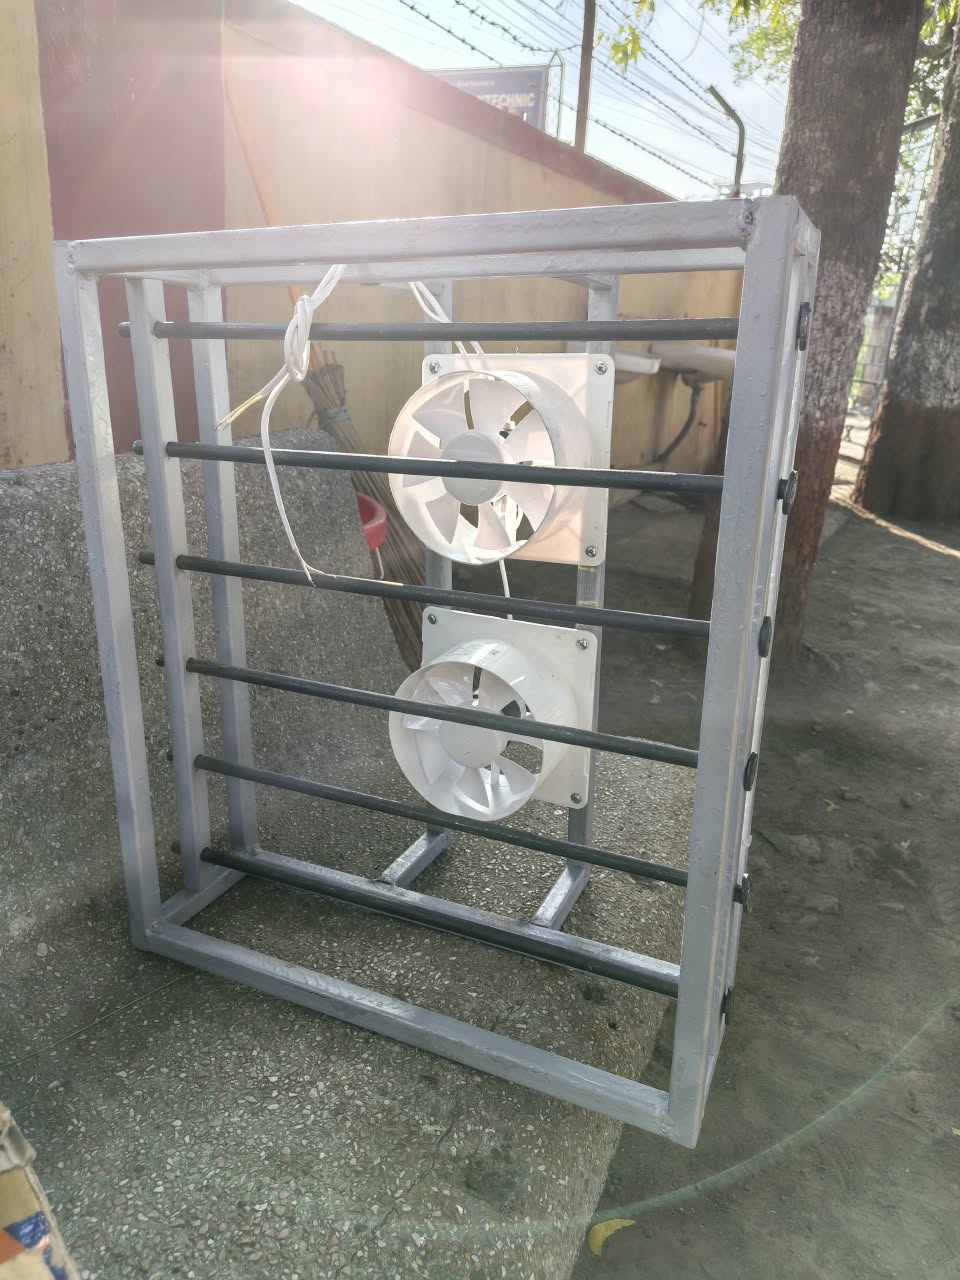
\includegraphics[width=\linewidth]{Frame_with_Rod_And_Exhaust_Fan_Colourd.jpeg}\caption{Painted, fans fitted}\end{subfigure}\hfill
\begin{subfigure}[b]{0.3\linewidth}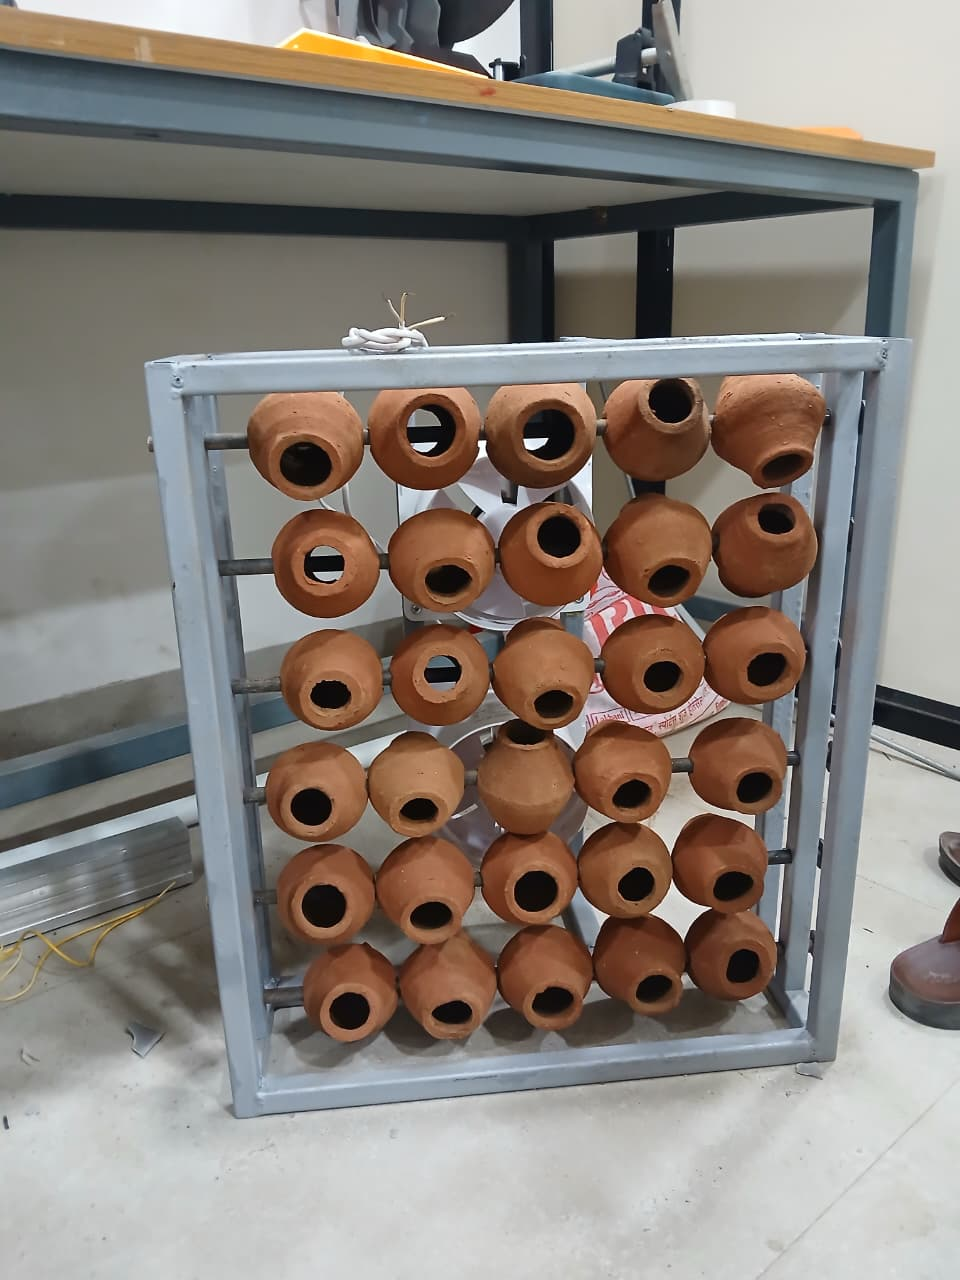
\includegraphics[width=\linewidth]{Frame_Completely_Assembled_Front_View.jpeg}\caption{30 pots, front}\end{subfigure}\hfill
\begin{subfigure}[b]{0.3\linewidth}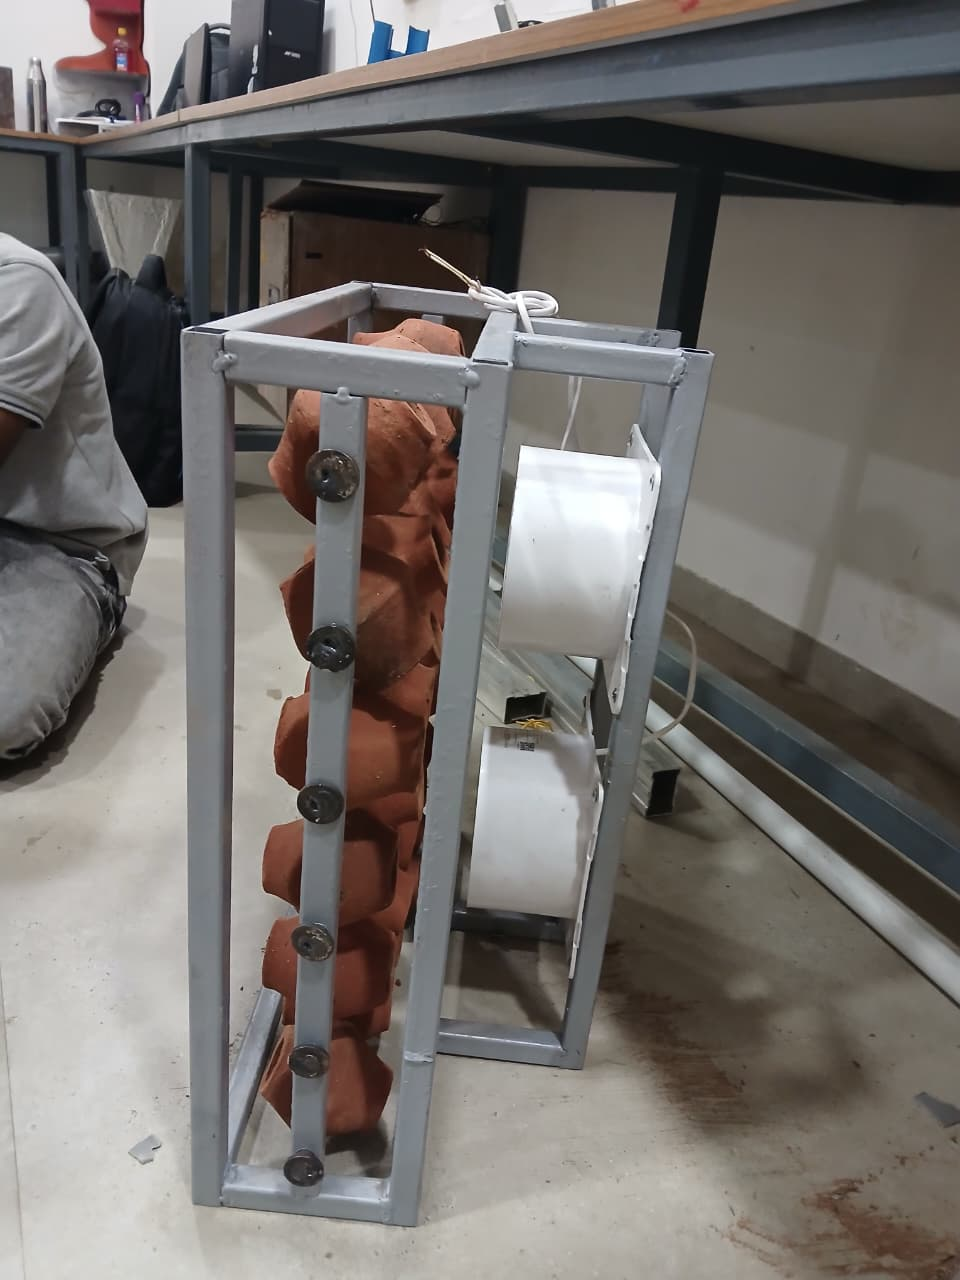
\includegraphics[width=\linewidth]{Frame_Completely_Assembled_Side_View.jpeg}\caption{Pots and fans, side}\end{subfigure}
\caption{Painted frame, fans and the 30-pot array.}
\label{fig:fab3}
\end{figure}

% ======================= 7 WATER SYSTEM =======================
\chapter{Water System}

The assembled frame stands inside a grey plastic tub that acts as the reservoir. A small pump in the tub (visible as a green unit with a black power cable in the front-right corner) lifts water through clear tubing that runs up a front post of the frame, through a blue connector, and along the top of the frame so water can wet the pots from above. Water that does not evaporate drains back into the tub (Figure~\ref{fig:water}).

\begin{figure}[H]
\centering
\begin{subfigure}[b]{0.32\linewidth}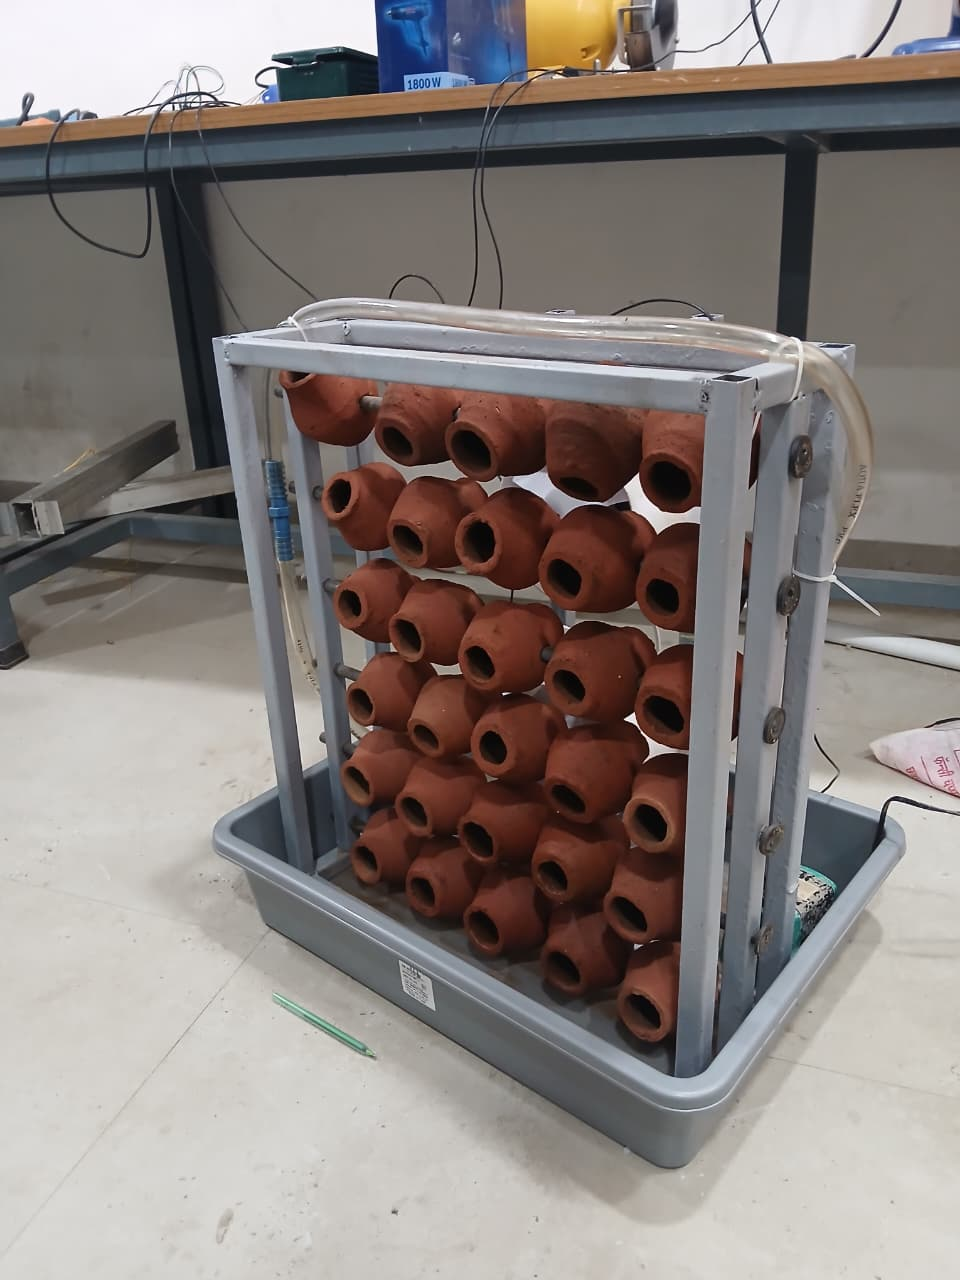
\includegraphics[width=\linewidth]{Water_System_Tub_Front_Right_View.jpeg}\caption{Front-right: tub, tubing, pump}\end{subfigure}\hfill
\begin{subfigure}[b]{0.32\linewidth}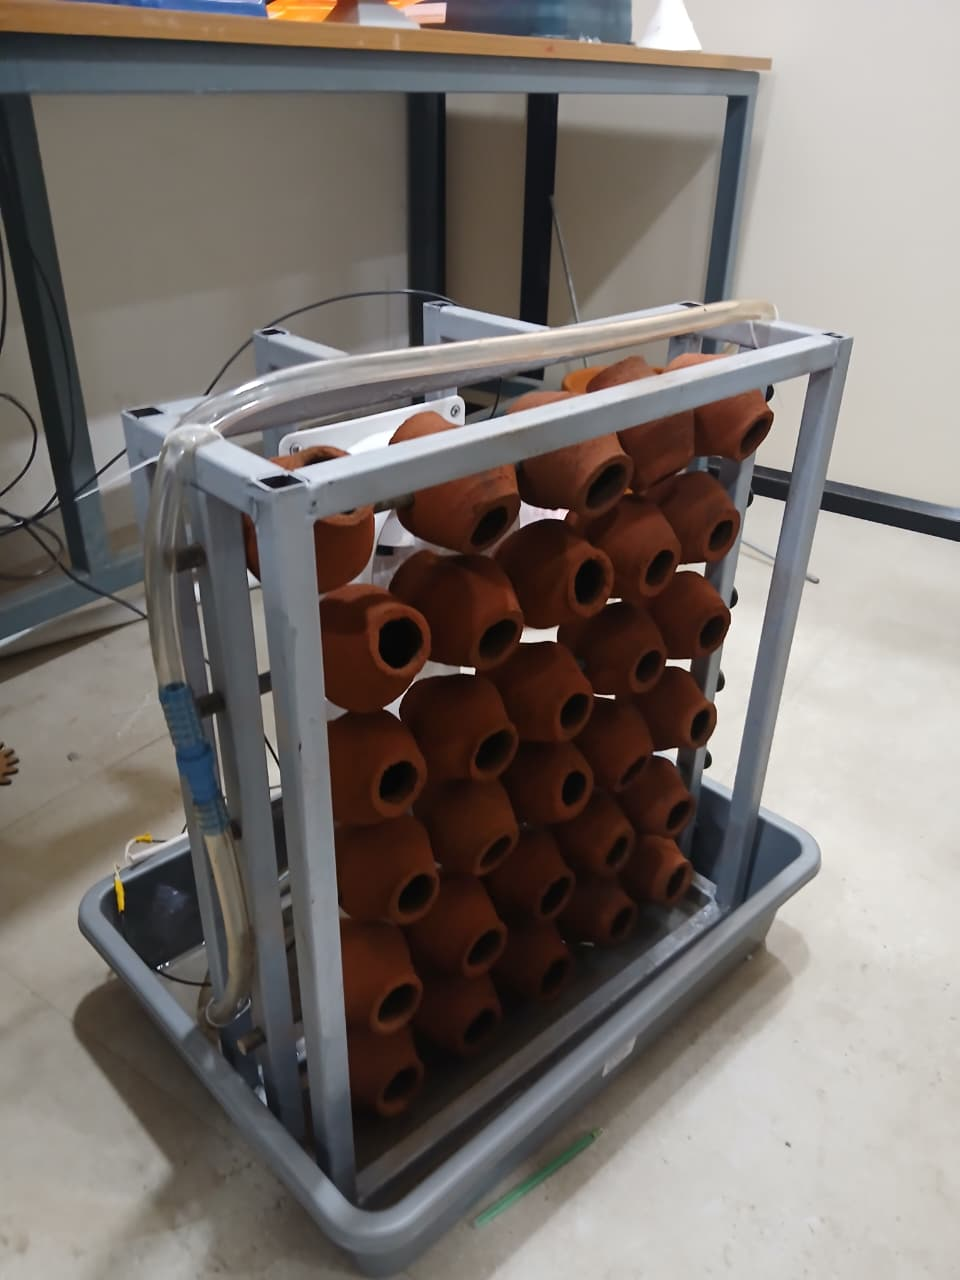
\includegraphics[width=\linewidth]{Water_System_Tub_Front_Left_View.jpeg}\caption{Front-left: tubing and connector}\end{subfigure}\hfill
\begin{subfigure}[b]{0.32\linewidth}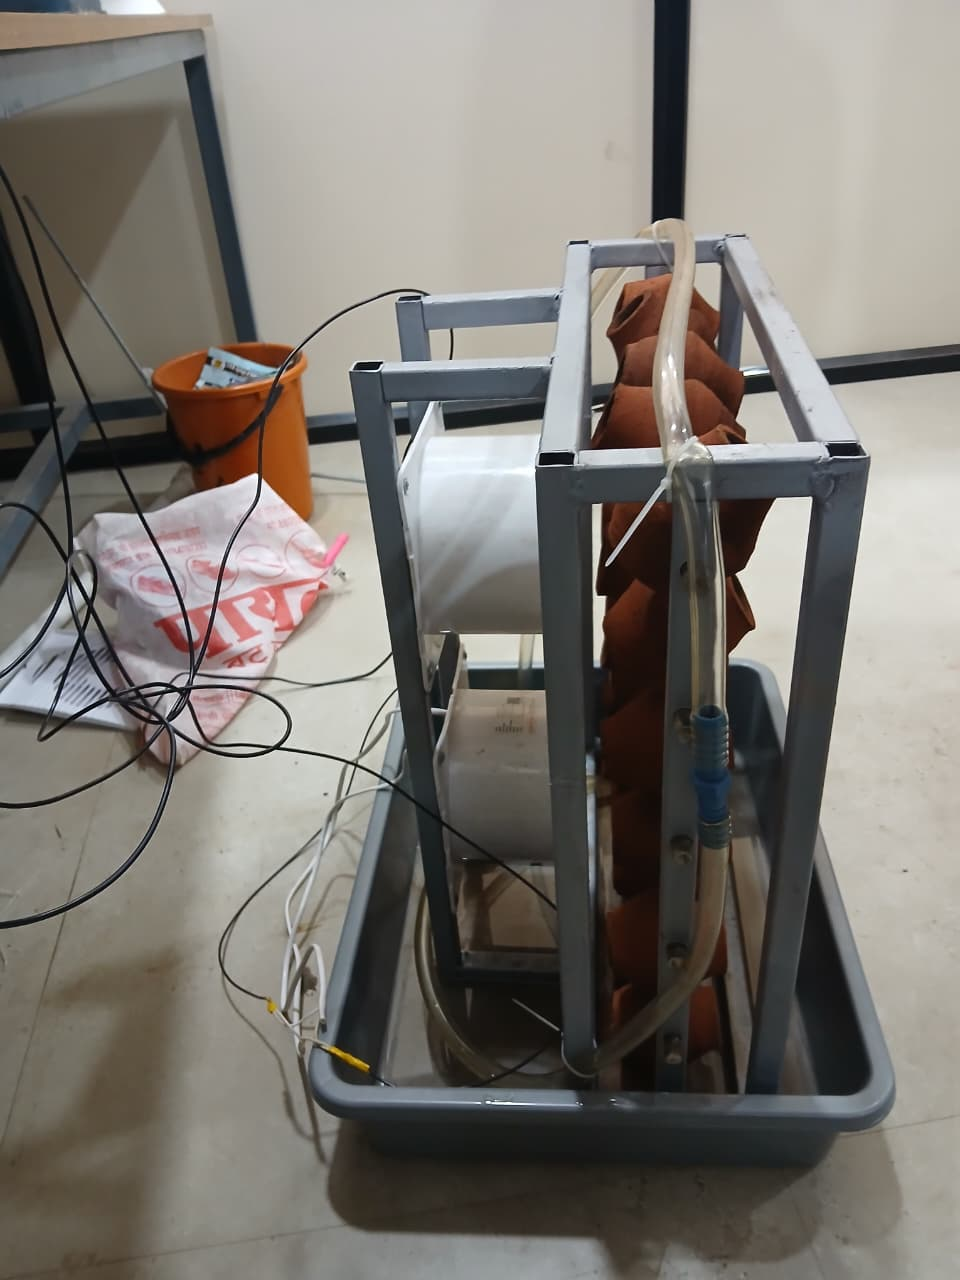
\includegraphics[width=\linewidth]{Water_System_Tub_Side_View.jpeg}\caption{Side: fans, tubing into tub}\end{subfigure}
\caption{The installed water system: the frame stands in the tub; tubing carries water from the pump to the top of the frame.}
\label{fig:water}
\end{figure}

\noindent Still to be recorded: tub dimensions and capacity, pump make, rating, flow and head, tubing length and bore, the distribution layout at the top, and a leak check. The supply cables beside the tub must be secured and kept clear of water.

% ======================= 8 ELECTRONICS =======================
\chapter{Electronics and Control Logic}
\label{ch:electronics}

\section{Architecture}
The ESP32 reads temperature and relative humidity from the DHT11 and drives a three-channel relay module that switches the two fans and the pump (Figure~\ref{fig:arch}). The figure is functional only; GPIO pins, relay channel mapping and wiring are not documented here and should be taken from the firmware and component datasheets.

\begin{figure}[H]
\centering
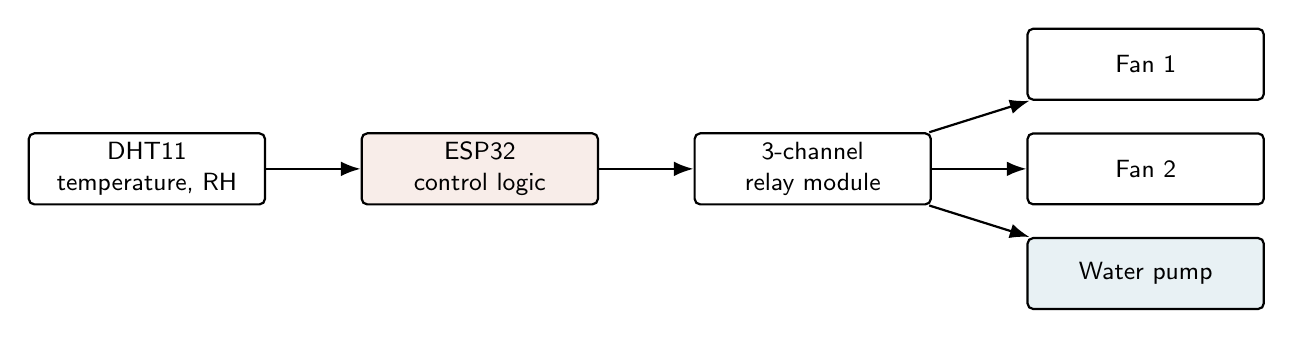
\begin{tikzpicture}[node distance=7mm and 12mm, every node/.style={font=\sffamily\small},
  box/.style={draw, rounded corners=2pt, minimum width=30mm, minimum height=9mm, align=center, line width=0.8pt},
  arr/.style={-{Latex[length=2.5mm]}, line width=0.8pt}]
  \node[box] (dht) {DHT11\\temperature, RH};
  \node[box, right=of dht, fill=cbclay!10] (esp) {ESP32\\control logic};
  \node[box, right=of esp] (relay) {3-channel\\relay module};
  \node[box, above right=4mm and 12mm of relay] (f1) {Fan 1};
  \node[box, right=12mm of relay] (f2) {Fan 2};
  \node[box, below right=4mm and 12mm of relay, fill=cbwater!10] (p) {Water pump};
  \draw[arr] (dht) -- (esp);
  \draw[arr] (esp) -- (relay);
  \draw[arr] (relay) -- (f1);
  \draw[arr] (relay) -- (f2);
  \draw[arr] (relay) -- (p);
\end{tikzpicture}
\caption{Functional architecture of the control electronics (not a wiring diagram).}
\label{fig:arch}
\end{figure}

\noindent\textbf{Enclosure (laser cutting in progress).} A laser-cut box will house the ESP32, the relay module and the DHT11 wiring: six finger-jointed panels for a 120 $\times$ 150 $\times$ 100\,mm box in 3\,mm MDF. The DXF is in the repository (\texttt{cad/dxf-enclosure/}); details in Section~\ref{sec:enclosure}.

\section{Implemented control logic}
\begin{table}[H]
\centering
\begin{minipage}[t]{0.47\linewidth}\centering
\caption{Fan control (temperature).}
\label{tab:fans}
\begin{tabular}{@{}ll@{}}
\toprule
\textbf{DHT11 temperature} & \textbf{Fans} \\
\midrule
$\le 28$\degC & Both OFF \\
$> 28$\degC{} and $\le 35$\degC & One fan ON \\
$> 35$\degC & Both fans ON \\
\bottomrule
\end{tabular}
\end{minipage}\hfill
\begin{minipage}[t]{0.47\linewidth}\centering
\caption{Pump control (humidity).}
\label{tab:pump}
\begin{tabular}{@{}ll@{}}
\toprule
\textbf{DHT11 relative humidity} & \textbf{Pump} \\
\midrule
$< 60$\,\% & ON \\
$\ge 60$\,\% & OFF \\
\bottomrule
\end{tabular}
\end{minipage}
\end{table}

\noindent At exactly 28.0\degC{} both fans are off; at exactly 35.0\degC{} one fan is on; at exactly 60.0\,\% RH the pump is off. Two physical points matter when interpreting this logic:
\begin{itemize}
\item Direct evaporative cooling has less potential in humid air~\cite{watson}, so stopping the pump at high RH avoids pumping water for little benefit.
\item Stopping the pump does not instantly dry the pots; their surfaces keep evaporating for some time, so humidity and cooling lag the pump's on/off state.
\end{itemize}

\section{Open engineering questions}
Sensor placement (ambient, inlet or outlet air), start-up behaviour before the first valid reading, rapid relay switching near the thresholds (hysteresis is not yet implemented), and whether the chosen thresholds are useful are all to be settled by testing. A browser simulation of this logic is available on the project website; it is software only and is not connected to the hardware.

% ======================= 9 SAFETY =======================
\chapter{Safety and Maintenance}

\section{Mechanical}
Inspect welds and joints before loading; remove burrs and sharp edges; check that rods hold the pots without point-loading or cracking them; keep the frame stable; secure the fans and guard accessible blades; isolate power before adjusting rods, fans, tubing or pots.

\section{Water and electrical}
Keep water, splashes and runoff away from fan motors, connectors, the relay and the ESP32. The breadboard electronics are not water-resistant and must be kept out of the drip path and later enclosed. Have any mains wiring and protective devices checked by a qualified person; do not rely on software as the only means of isolation; never handle wiring with wet hands; de-energise before refilling, cleaning or repairing leaks; do not run the pump dry or against a blocked outlet.

\section{Hygiene and maintenance}
Use clean water and drain the tub when the cooler will be idle, so water does not stagnate. Inspect the tub, tubing and pots for deposits, slime, blockages, cracks and leaks, and clean them with methods compatible with the clay and pump~\cite{doe}. Record cracked pots, corrosion, loose fasteners and changes in flow or fan noise.

% ======================= 10 TESTING =======================
\chapter{Testing Plan}
\label{ch:testing}

\section{Test conditions}
Two conditions will be compared, keeping fan settings, sensor positions and test duration the same: (1) a \textbf{fan-only / dry-pot baseline} with the pump off, and (2) a \textbf{wetted-pot condition} with the pump and fans running. Ambient temperature, relative humidity, location, sun and wind will be recorded for every run, and runs repeated where possible.

\section{Measurements}
\begin{table}[H]
\centering
\caption{Planned measurements.}
\label{tab:measure}
\small
\begin{tabularx}{\linewidth}{@{}>{\raggedright\arraybackslash}p{3.6cm}>{\raggedright\arraybackslash}X@{}}
\toprule
\textbf{Quantity} & \textbf{Method} \\
\midrule
Inlet temperature and RH & Behind the rear fans, where room air enters; away from wet clay. \\
Outlet temperature and RH & In front of the pots at documented points; several points if flow is uneven. \\
Ambient conditions & Near the setup, outside the wet airstream. \\
Air velocity & Anemometer at documented points, if available (a point velocity is not total flow). \\
Water use & Tub level or mass at start and end of a timed run; leaks and refills noted separately. \\
Electrical input & Nameplate ratings, and measured power with a suitable meter if available and safe. \\
Control behaviour & Fan stage and pump state against the DHT11 reading and a reference hygrometer/thermometer. \\
Wetting and return flow & Photographs of wetting pattern, dry spots, leaks and return flow. \\
\bottomrule
\end{tabularx}
\end{table}

\section{Calculations}
Once reliable measurements exist:
\begin{align*}
\Delta T &= T_\text{inlet} - T_\text{outlet} \\
\Delta RH &= RH_\text{outlet} - RH_\text{inlet} \quad \text{(percentage points)}\\
\text{Water-use rate} &= \frac{\text{net water loss}}{\text{test duration}} \\
\text{Electrical energy} &= \bar{P} \times t
\end{align*}
A positive $\Delta T$ shows that outlet air was cooler than inlet air for that run; it does not by itself establish room-wide cooling or superiority over another cooler. RH must be interpreted with the simultaneous temperatures.

% ======================= 11 RESULTS =======================
\chapter{Results}

\begin{center}
\fbox{\begin{minipage}{0.9\linewidth}\centering\vspace{3mm}
\textbf{Results: to be measured.}\\[2mm]
Performance testing is in progress. No temperature, humidity, airflow, water-use, power or cost results have been recorded, and none are reported here. Results will be added only from real measurements, with the raw data and the test conditions.
\vspace{3mm}\end{minipage}}
\end{center}

\begin{table}[H]
\centering
\caption{Results template (to be filled from measurements).}
\label{tab:results}
\small
\begin{tabular}{@{}lccccccc@{}}
\toprule
\textbf{Run} & \textbf{Mode} & $T_\text{in}$ & $T_\text{out}$ & $RH_\text{in}$ & $RH_\text{out}$ & \textbf{Water} & \textbf{Power} \\
 & & (\textdegree C) & (\textdegree C) & (\%) & (\%) & (L/h) & (W) \\
\midrule
1 & Dry baseline & -- & -- & -- & -- & -- & -- \\
2 & Wetted pots & -- & -- & -- & -- & -- & -- \\
\bottomrule
\end{tabular}
\end{table}

What \emph{has} been verified is qualitative: the prototype is fully assembled, and the control logic is running on the ESP32, switching the fans and the pump.

% ======================= 12 CHALLENGES =======================
\chapter{Challenges}
\begin{itemize}
\item Cutting and welding the square pipe so the frame stays square and true to the design size.
\item Marking and drilling rod holes in line on opposite members so the rods pass straight through.
\item Supporting 30 fragile clay pots securely without cracking them.
\item Routing tubing so water reaches the top of the pot array and drains back to the tub.
\item Keeping the breadboard electronics and supply cables away from water.
\item Choosing thresholds for the temperature-staged fans and the humidity-based pump.
\item Keeping the CAD model in step with the physical build.
\end{itemize}

% ======================= 13 CONCLUSION =======================
\chapter{Conclusion and Future Scope}

\section{Conclusion}
ClayBreeze addresses a real problem --- affordable cooling for hot Indian homes, classrooms and workshops --- by replacing the consumable cooler pad with porous, unglazed terracotta pots, kept wet by a recirculating water system and controlled by an ESP32. The frame, 30 pots, fans, tub, pump and tubing are complete, and the temperature-staged fan control and humidity-based pump control are running. The design aims of low cost, low power, no pad replacement and an eco-friendly build are \emph{plausible but unproven}: they will be confirmed or rejected by the tests in Chapter~\ref{ch:testing}.

\section{Future scope}
\begin{itemize}
\item Run dry-baseline and wetted-pot tests: inlet/outlet temperature and RH, airflow, water use and electrical power.
\item Add an even top water-distribution header and complete a leak check.
\item Move the electronics to a PCB in a splash-proof enclosure; add fan guards.
\item Add hysteresis to the thresholds, a water-level sensor in the tub and a dry-run cut-out for the pump.
\item Study other pot sizes, spacings and clay bodies.
\item Record costs from receipts; update the SolidWorks model and drawing to the as-built prototype.
\end{itemize}

\section*{Project links}
\begin{itemize}
\item Live website (3D model, photos, docs): \url{https://tanmay-np.github.io/Claybreeze-Sustainable-Air-Cooling/}
\item GitHub repository: \url{https://github.com/tanmay-np/Claybreeze-Sustainable-Air-Cooling}
\end{itemize}

% ======================= 14 MAKERSPACE WORKBENCH =======================
\chapter{Makerspace Workbench --- 3D Printing \& Laser Cutting at Tinkerers' Lab}
\label{ch:digifab}

This chapter records the 3D printing and laser cutting skills learned and practised at Tinkerers' Lab, Sanjivani University, and where they feed back into ClayBreeze. The lab has four Bambu Lab printers that use \textbf{FDM --- Fused Deposition Modelling (also called FFF, Fused Filament Fabrication)} and a \textbf{CO$_2$ (carbon dioxide) laser cutter}. Learning reference: Dr.\ Kiran Wakchaure's Fab Academy documentation~\cite{wakchaure}; everything here is in our own words. Practice pieces are done, and the ClayBreeze electronics enclosure is being laser-cut now (Section~\ref{sec:enclosure}).

\begin{table}[H]
\centering\small
\caption{Abbreviations used in this chapter.}
\begin{tabular}{@{}ll@{\hspace{8mm}}ll@{}}
\toprule
FDM & Fused Deposition Modelling & ASA & Acrylonitrile styrene acrylate \\
FFF & Fused Filament Fabrication & TPU & Thermoplastic polyurethane \\
CAD & Computer-Aided Design & AMS & Automatic Material System \\
STL & Stereolithography (triangle-mesh file) & DXF & Drawing Exchange Format \\
3MF & 3D Manufacturing Format & SVG & Scalable Vector Graphics \\
PLA & Polylactic acid & CO$_2$ & Carbon dioxide \\
PETG & Polyethylene terephthalate glycol-modified & PPI & Pulses per inch \\
ABS & Acrylonitrile butadiene styrene & MDF & Medium-density fibreboard \\
\bottomrule
\end{tabular}
\end{table}

\begin{figure}[H]
\centering
\begin{subfigure}[b]{0.24\linewidth}\centering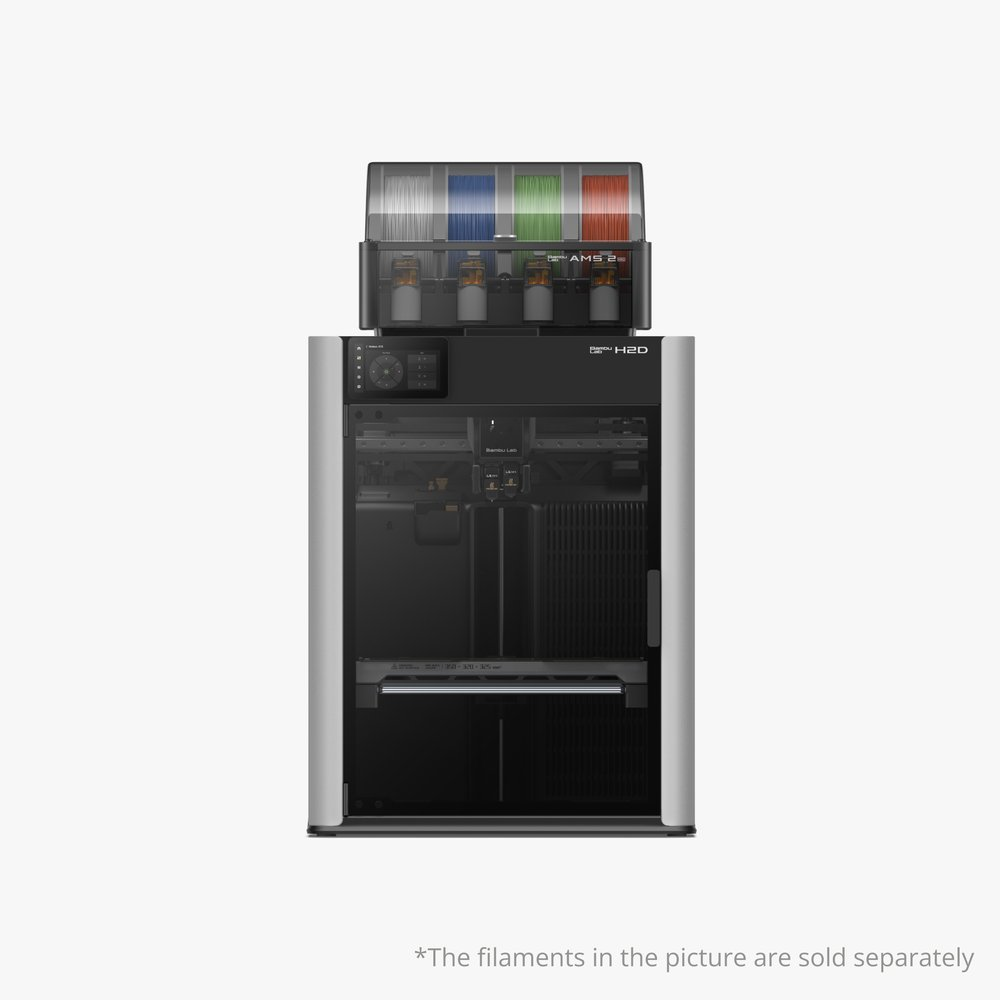
\includegraphics[width=\linewidth]{bambu/h2d.jpg}\caption{H2D --- dual-nozzle enclosed flagship}\end{subfigure}\hfill
\begin{subfigure}[b]{0.24\linewidth}\centering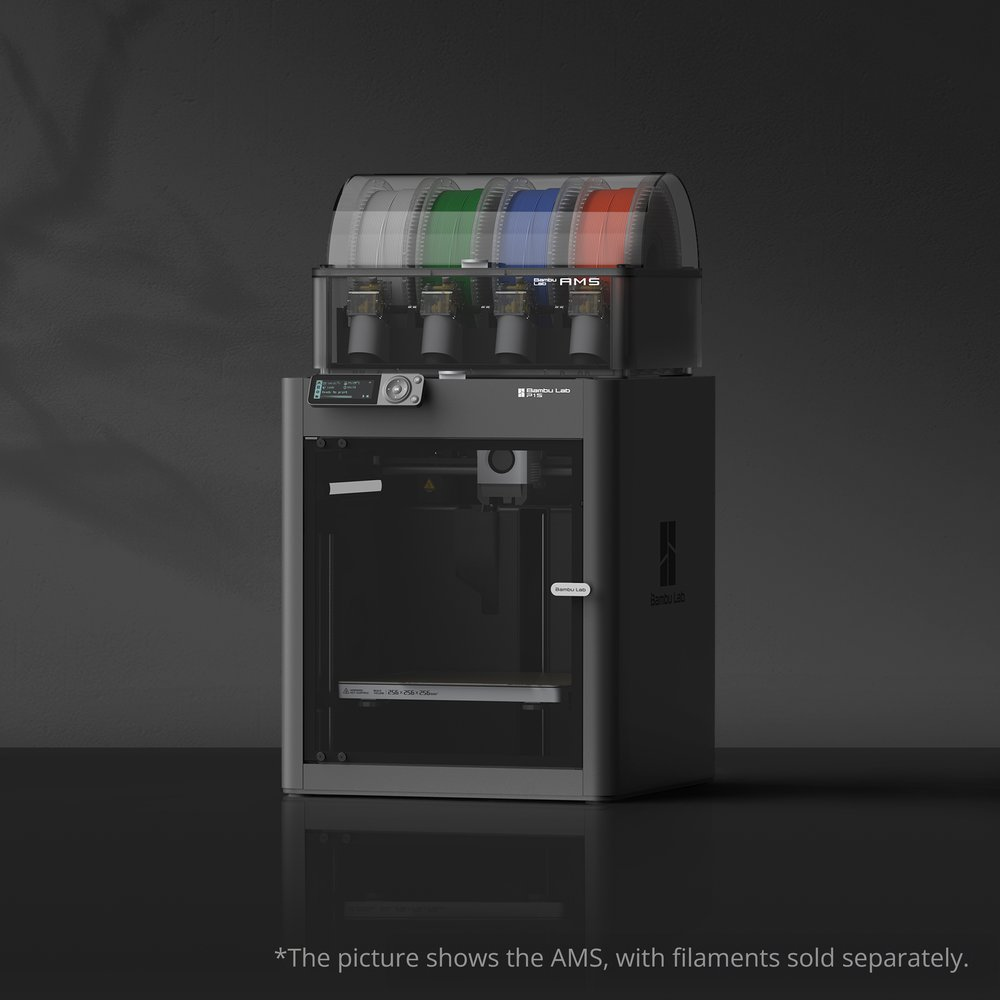
\includegraphics[width=\linewidth]{bambu/p1s.jpg}\caption{P1S --- enclosed all-rounder}\end{subfigure}\hfill
\begin{subfigure}[b]{0.24\linewidth}\centering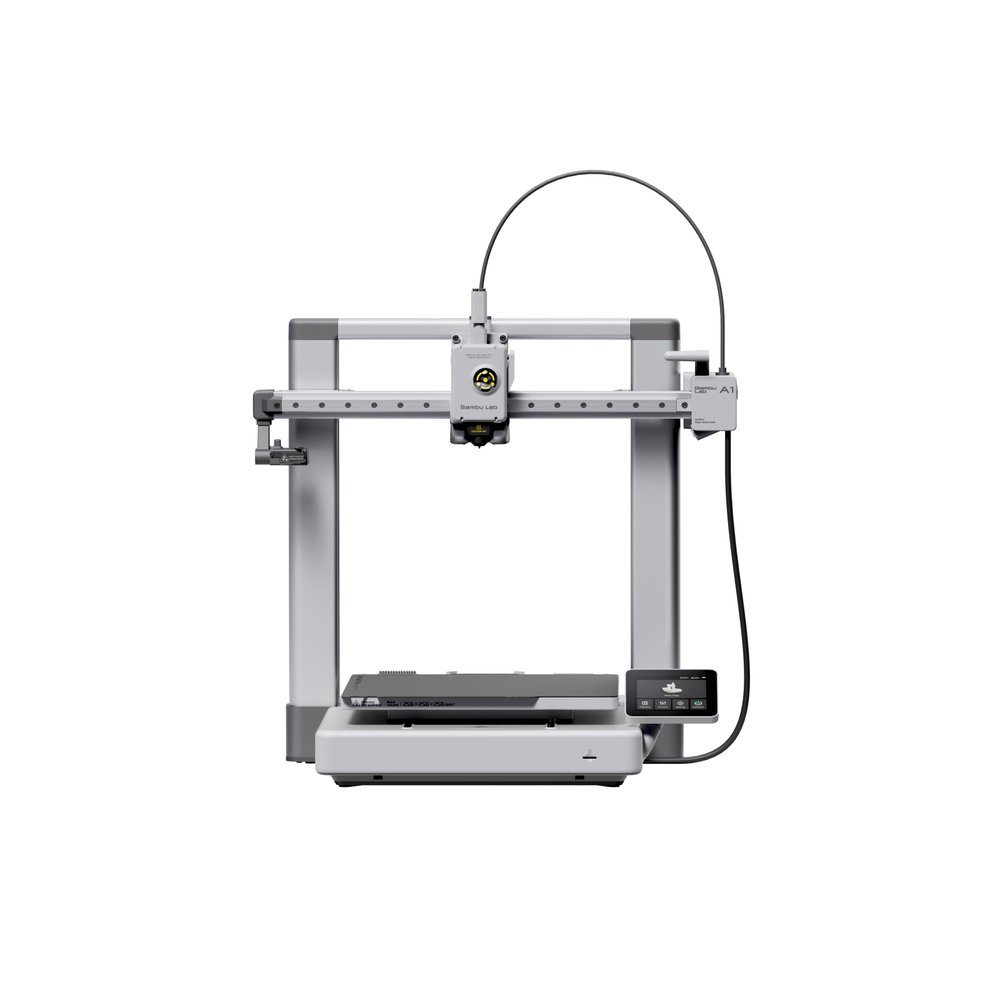
\includegraphics[width=\linewidth]{bambu/a1.jpg}\caption{A1 --- open-frame workhorse}\end{subfigure}\hfill
\begin{subfigure}[b]{0.24\linewidth}\centering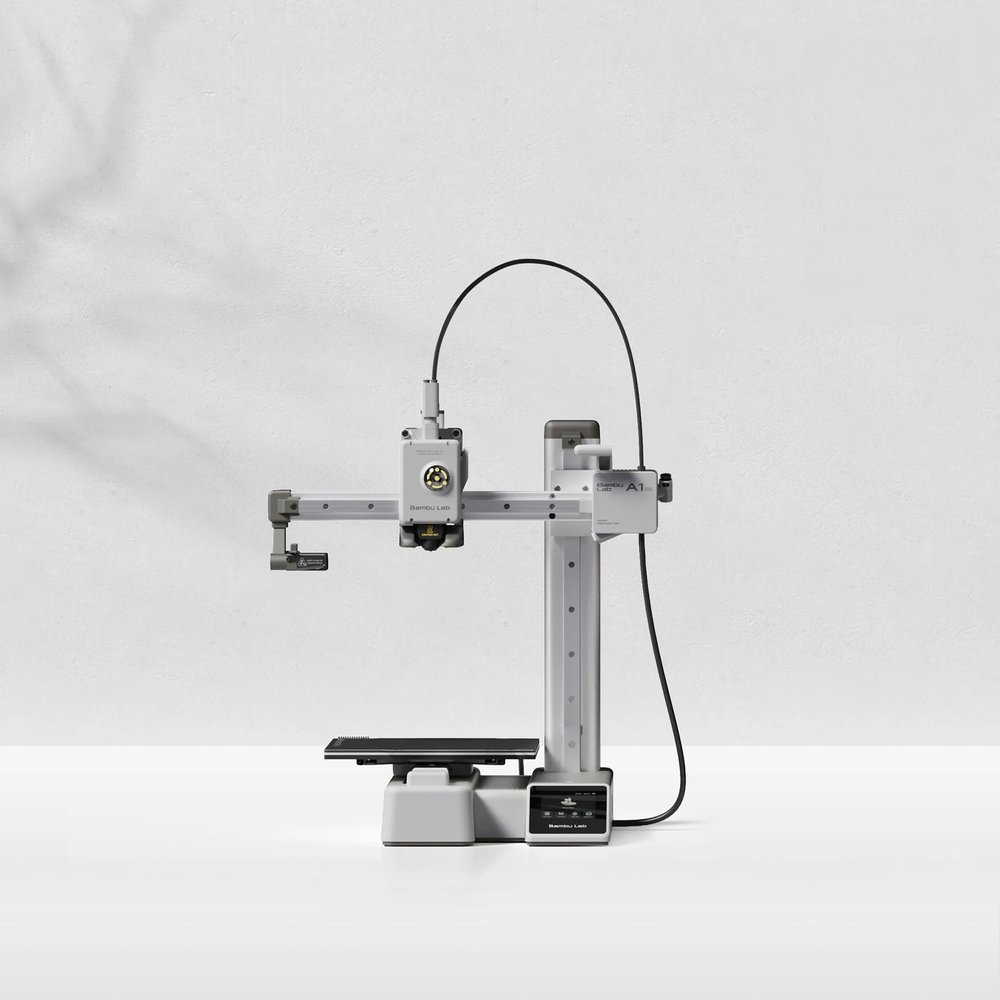
\includegraphics[width=\linewidth]{bambu/a1-mini.jpg}\caption{A1 mini --- compact starter}\end{subfigure}
\caption{The four Bambu Lab printers at Tinkerers' Lab. Images: \textcopyright\ Bambu Lab, official store pages~\cite{bambuimages}.}
\label{fig:bambu}
\end{figure}

\section{3D printing: FDM --- Fused Deposition Modelling (also called FFF, Fused Filament Fabrication)}
An FDM printer melts a plastic wire called filament and lays it down line by line, layer by layer.
\textbf{Workflow:} CAD model $\rightarrow$ export STL or 3MF $\rightarrow$ slice in Bambu Studio $\rightarrow$ print, watching the first layer $\rightarrow$ post-process (cool, release, remove supports and brim, smooth, test-fit).

\subsection{Two ways an FDM printer moves}
Every FDM printer must move the nozzle relative to the part in X (left--right), Y (front--back) and Z (up, one layer at a time). Our printers use two motion systems (Figure~\ref{fig:motion}, Table~\ref{tab:motion}). The classification was checked against Bambu Lab sources: the A1 and A1 mini product pages call them ``bed slinger'' printers~\cite{bambua1,bambua1mini}, the P1 series page states CoreXY~\cite{bambup1s}, and the Bambu Lab Wiki states that the H2D ``is based on the Core-XY architecture''~\cite{bambuh2dwiki}.

\begin{figure}[H]
\centering
\begin{subfigure}[b]{0.49\linewidth}\centering
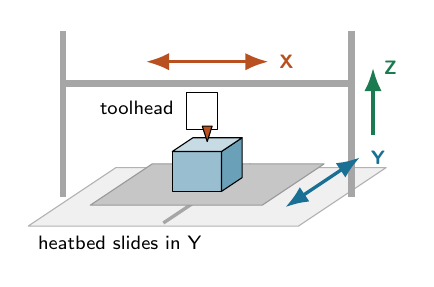
\begin{tikzpicture}[x={(1cm,0)}, y={(0.42cm,0.28cm)}, z={(0,1cm)}, scale=0.78, font=\sffamily\scriptsize, line join=round]
  \draw[fill=gray!12, draw=gray!60] (0,-0.4,0) -- (4.4,-0.4,0) -- (4.4,3.0,0) -- (0,3.0,0) -- cycle;
  \draw[gray!70, line width=1.2pt] (2.2,-0.4,0.05) -- (2.2,3.0,0.05);
  \draw[line width=2.4pt, gray!70] (-0.15,1.3,0) -- (-0.15,1.3,2.7);
  \draw[line width=2.4pt, gray!70] (4.55,1.3,0) -- (4.55,1.3,2.7);
  \draw[fill=gray!45, draw=gray!80] (0.8,0.1,0.2) -- (3.6,0.1,0.2) -- (3.6,2.5,0.2) -- (0.8,2.5,0.2) -- cycle;
  \draw[fill=cbwater!45] (1.8,0.9,0.2) -- (2.6,0.9,0.2) -- (2.6,0.9,0.85) -- (1.8,0.9,0.85) -- cycle;
  \draw[fill=cbwater!65] (2.6,0.9,0.2) -- (2.6,1.7,0.2) -- (2.6,1.7,0.85) -- (2.6,0.9,0.85) -- cycle;
  \draw[fill=cbwater!25] (1.8,0.9,0.85) -- (2.6,0.9,0.85) -- (2.6,1.7,0.85) -- (1.8,1.7,0.85) -- cycle;
  \draw[line width=2.4pt, gray!70] (-0.15,1.3,1.85) -- (4.55,1.3,1.85);
  \draw[fill=white] (1.95,1.1,1.15) -- (2.45,1.1,1.15) -- (2.45,1.1,1.75) -- (1.95,1.1,1.75) -- cycle;
  \draw[fill=cbclay] (2.12,1.3,1.15) -- (2.28,1.3,1.15) -- (2.2,1.3,0.9) -- cycle;
  \draw[{Latex}-{Latex}, cbclay, very thick] (1.2,1.3,2.2) -- (3.2,1.3,2.2) node[right]{\textbf{X}};
  \draw[{Latex}-{Latex}, cbwater, very thick] (4.1,-0.2,0.25) -- (4.1,2.7,0.25) node[right]{\textbf{Y}};
  \draw[-{Latex}, cbok, very thick] (4.9,1.3,1.0) -- (4.9,1.3,2.1) node[right]{\textbf{Z}};
  \node[anchor=north west, align=left] at (0,-0.4,0) {heatbed slides in Y};
  \node[anchor=east, align=right] at (1.9,1.1,1.5) {toolhead};
\end{tikzpicture}
\caption{Bed-slinger (Cartesian): the \textcolor{cbwater}{heatbed moves front--back (Y)}, the \textcolor{cbclay}{toolhead moves left--right (X)}, the \textcolor{cbok}{toolhead and gantry rise (Z)}. Our lab: A1, A1 mini.}
\end{subfigure}\hfill
\begin{subfigure}[b]{0.49\linewidth}\centering
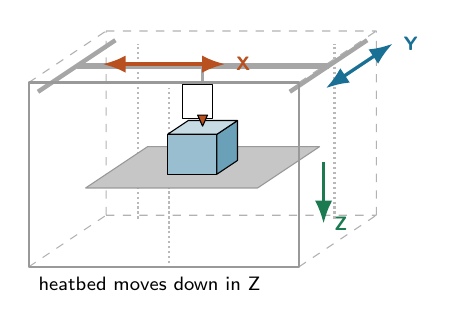
\begin{tikzpicture}[x={(1cm,0)}, y={(0.42cm,0.28cm)}, z={(0,1cm)}, scale=0.78, font=\sffamily\scriptsize, line join=round]
  \draw[gray!60, dashed] (0,3,0) -- (4.4,3,0) (0,3,0) -- (0,3,3) (4.4,3,0) -- (4.4,3,3) (0,0,0) -- (0,3,0) (4.4,0,0) -- (4.4,3,0) (0,0,3) -- (0,3,3) (4.4,0,3) -- (4.4,3,3) (0,3,3) -- (4.4,3,3);
  \draw[gray!55, densely dotted, thick] (0.6,2.8,0) -- (0.6,2.8,2.85) (3.8,2.8,0) -- (3.8,2.8,2.85) (2.2,0.2,0) -- (2.2,0.2,2.85);
  \draw[line width=1.6pt, gray!70] (0.15,0,2.85) -- (0.15,3,2.85) (4.25,0,2.85) -- (4.25,3,2.85);
  \draw[fill=gray!45, draw=gray!80] (0.8,0.3,1.2) -- (3.6,0.3,1.2) -- (3.6,2.7,1.2) -- (0.8,2.7,1.2) -- cycle;
  \draw[fill=cbwater!45] (1.8,1.1,1.2) -- (2.6,1.1,1.2) -- (2.6,1.1,1.85) -- (1.8,1.1,1.85) -- cycle;
  \draw[fill=cbwater!65] (2.6,1.1,1.2) -- (2.6,1.9,1.2) -- (2.6,1.9,1.85) -- (2.6,1.1,1.85) -- cycle;
  \draw[fill=cbwater!25] (1.8,1.1,1.85) -- (2.6,1.1,1.85) -- (2.6,1.9,1.85) -- (1.8,1.9,1.85) -- cycle;
  \draw[line width=2.4pt, gray!70] (0.15,1.5,2.85) -- (4.25,1.5,2.85);
  \draw[gray!70, thick] (2.2,1.5,2.85) -- (2.2,1.5,2.6);
  \draw[fill=white] (1.95,1.3,2.05) -- (2.45,1.3,2.05) -- (2.45,1.3,2.6) -- (1.95,1.3,2.6) -- cycle;
  \draw[fill=cbclay] (2.12,1.5,2.05) -- (2.28,1.5,2.05) -- (2.2,1.5,1.87) -- cycle;
  \draw[gray!80, thick] (0,0,0) rectangle (4.4,0,3);
  \draw[{Latex}-{Latex}, cbclay, very thick] (1.2,0,3.3) -- (3.2,0,3.3) node[right]{\textbf{X}};
  \draw[{Latex}-{Latex}, cbwater, very thick] (4.75,0.2,2.85) -- (4.75,2.8,2.85) node[right]{\textbf{Y}};
  \draw[-{Latex}, cbok, very thick] (4.8,0,1.7) -- (4.8,0,0.7) node[right]{\textbf{Z}};
  \node[anchor=north west] at (0,0,0) {heatbed moves down in Z};
\end{tikzpicture}
\caption{CoreXY (enclosed): the \textcolor{cbclay}{toolhead moves in X} and \textcolor{cbwater}{Y} on a fixed frame; the \textcolor{cbok}{heatbed moves down (Z)} after each layer. Our lab: P1S, H2D.}
\end{subfigure}
\caption{The two FDM motion systems in our lab, printing the same part (layer height exaggerated). The website animates both side by side.}
\label{fig:motion}
\end{figure}

\begin{table}[H]
\centering\small
\caption{Bed-slinger vs CoreXY.}
\label{tab:motion}
\begin{tabularx}{\linewidth}{@{}>{\bfseries}lXX@{}}
\toprule
 & \textbf{Bed-slinger (Cartesian)} & \textbf{CoreXY (enclosed)} \\
\midrule
X (left--right) & Toolhead moves along the gantry & Toolhead moves on a fixed frame at the top \\
Y (front--back) & Heatbed slides; the part rides on it & Toolhead moves; two fixed motors and crossed belts drive X and Y together \\
Z (each layer) & Toolhead and gantry rise & Heatbed moves down \\
Our lab & A1, A1 mini & P1S, H2D \\
\bottomrule
\end{tabularx}
\end{table}

\subsection{How FDM works}
\begin{enumerate}[itemsep=1pt]
\item \textbf{Filament feeds from the spool} --- the 1.75\,mm filament is pulled through a tube only as fast as the nozzle uses it.
\item \textbf{Extruder gears push it} --- two toothed gears grip the filament and push it at an exact rate; they pause on travel moves and retract slightly to stop drips.
\item \textbf{The hotend melts it} --- about 190--240\degC{} for PLA~\cite{bambuwiki}; a cooled heat break keeps the filament solid until the hot zone.
\item \textbf{The nozzle traces the toolpath} --- molten plastic leaves the 0.4\,mm nozzle as a thin line along the slicer's path.
\item \textbf{Layers stack} --- after each layer the gantry rises (bed-slinger) or the bed lowers (CoreXY) by one layer height.
\item \textbf{The cooling fan sets each line} --- the part-cooling fan hardens the fresh plastic so it holds its shape.
\end{enumerate}

\begin{figure}[H]
\centering
\begin{minipage}[c]{0.5\linewidth}
\centering
\begin{tikzpicture}
\node[anchor=south west, inner sep=0] (img) {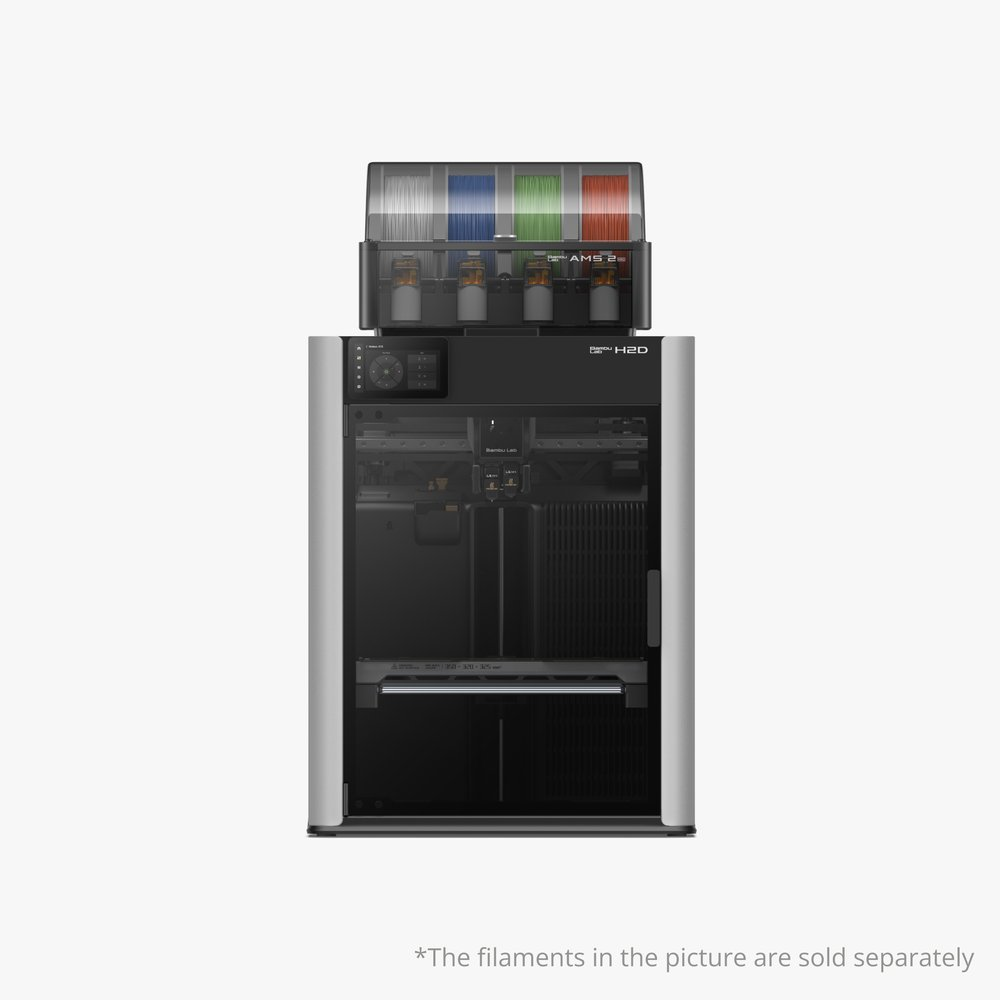
\includegraphics[width=\linewidth]{bambu/h2d.jpg}};
\begin{scope}[x={(img.south east)}, y={(img.north west)}]
\foreach \n/\x/\y in {1/0.500/0.503, 2/0.500/0.575, 3/0.446/0.330, 4/0.595/0.560, 5/0.652/0.393, 6/0.429/0.633, 7/0.500/0.795, 8/0.357/0.585}
  \node[circle, fill=cbclay, draw=white, line width=0.6pt, text=white, font=\scriptsize\bfseries, inner sep=1.2pt, minimum size=11pt] at (\x,\y) {\n};
\end{scope}
\end{tikzpicture}
\end{minipage}\hfill
\begin{minipage}[c]{0.46\linewidth}
\small
\begin{enumerate}[leftmargin=*, itemsep=1pt]
\item \textbf{Dual nozzles and hotend} --- melt the filament (up to 350\degC); two materials or colours in one print.
\item \textbf{Extruder} --- gears push filament into the hotend at a controlled rate.
\item \textbf{Heated build plate} --- holds the first layer down (up to 120\degC).
\item \textbf{Motion system (CoreXY)} --- two fixed motors and crossed belts move the head in X and Y; the plate steps down each layer.
\item \textbf{Enclosure and door} --- keep warm air in (chamber heating to 65\degC).
\item \textbf{Touchscreen} --- start prints, load filament, read errors.
\item \textbf{Filament and AMS} --- the AMS 2 Pro holds four spools and feeds them automatically.
\item \textbf{Camera and lighting} --- built-in cameras and chamber light (position approximate).
\end{enumerate}
\end{minipage}
\caption{Labelled parts of the Bambu Lab H2D (numbers added by us; positions approximate). Image: \textcopyright\ Bambu Lab~\cite{bambuimages}.}
\label{fig:h2dlabels}
\end{figure}

\begin{table}[H]
\centering\small
\caption{Key FDM print settings, one line each.}
\begin{tabularx}{\linewidth}{@{}>{\bfseries\raggedright\arraybackslash}p{0.22\linewidth}X@{}}
\toprule
Setting & \textbf{What it does} \\
\midrule
Layer height & Thickness of each layer; thinner is smoother but slower (0.2\,mm usual for a 0.4\,mm nozzle). \\
Nozzle diameter / temp. & Line width (0.4\,mm standard); temperature set for the material --- too cold gives weak layers, too hot gives strings. \\
Extruder & Gears that push filament into the hotend; ``direct drive'' means they sit on the print head. \\
Bed and build plate & A heated plate keeps the first layer down; the surface is chosen for the material. \\
Infill & The inside fill of a part, as a percentage and a pattern; more is stronger but slower. \\
Perimeter (wall) & An outline loop around each layer; most of a part's strength comes from the perimeters. \\
Support & Temporary scaffolding printed under overhangs and removed afterwards. \\
Brim & Extra flat loops around the first layer that help small or tall parts stay stuck. \\
Raft & A throw-away base printed under the whole part; rarely needed on modern plates. \\
Speed, cooling fan & Faster saves time but can cost quality; the fan hardens each line (high for PLA, low for ABS/ASA). \\
\bottomrule
\end{tabularx}
\end{table}

\begin{table}[H]
\centering\small
\caption{Filaments, from Bambu Lab's filament guide~\cite{bambuwiki} (nozzle ranges $\pm$10\degC; ratings are heat resistance / impact / tensile strength). ``Good for'' is our summary.}
\begin{tabularx}{\linewidth}{@{}lllXl@{}}
\toprule
Material & Nozzle & Bed & Printer & Ratings \\
\midrule
PLA & 190--240\degC & 35--65\degC & Open or enclosed. Good for prototypes, models, jigs. & 2 / 2 / 3 \\
PETG & 240--270\degC & 60--80\degC & Open or enclosed. Functional parts, parts near water. & 3 / 3 / 2 \\
ABS & 240--280\degC & 90--100\degC & Enclosed recommended (fumes). Parts that get warm. & 3 / 3 / 3 \\
ASA & 240--280\degC & 90--100\degC & Enclosed recommended (fumes). Outdoor parts. & 3 / 3 / 3 \\
TPU 95A HF & 200--250\degC & 30--45\degC & Open or enclosed. Flexible parts; too soft for most AMS use. & not rated \\
\bottomrule
\end{tabularx}
\end{table}

\begin{table}[H]
\centering\small
\caption{Lab printers, from official Bambu Lab pages~\cite{bambuh2d,bambup1s,bambua1,bambua1mini,bambuh2dwiki}.}
\begin{tabularx}{\linewidth}{@{}>{\raggedright\arraybackslash}p{0.17\linewidth}>{\raggedright\arraybackslash}X>{\raggedright\arraybackslash}p{0.15\linewidth}>{\raggedright\arraybackslash}p{0.15\linewidth}>{\raggedright\arraybackslash}p{0.15\linewidth}@{}}
\toprule
 & H2D & P1S & A1 & A1 mini \\
\midrule
Motion system & CoreXY & CoreXY & Bed-slinger & Bed-slinger \\
Build volume (mm) & 325$\times$320$\times$325 (one nozzle); 300$\times$320$\times$320 (both) & 256$\times$256$\times$256 & 256$\times$256$\times$256 & 180$\times$180$\times$180 \\
Enclosure & Enclosed, chamber heating to 65\degC & Enclosed & Open frame (see manufacturer) & Open frame (see manufacturer) \\
Nozzle(s) & Two, 0.4\,mm included & One, 0.4\,mm & One, 0.4\,mm & One, 0.4\,mm \\
Max nozzle temp. & 350\degC & 300\degC & 300\degC & 300\degC \\
Max bed temp. & 120\degC & 100\degC & 100\degC & 80\degC \\
AMS support & AMS 2 Pro, AMS HT & AMS & AMS lite & AMS lite \\
\bottomrule
\end{tabularx}
\end{table}

\begin{figure}[H]
\centering
\begin{subfigure}[b]{0.24\linewidth}\centering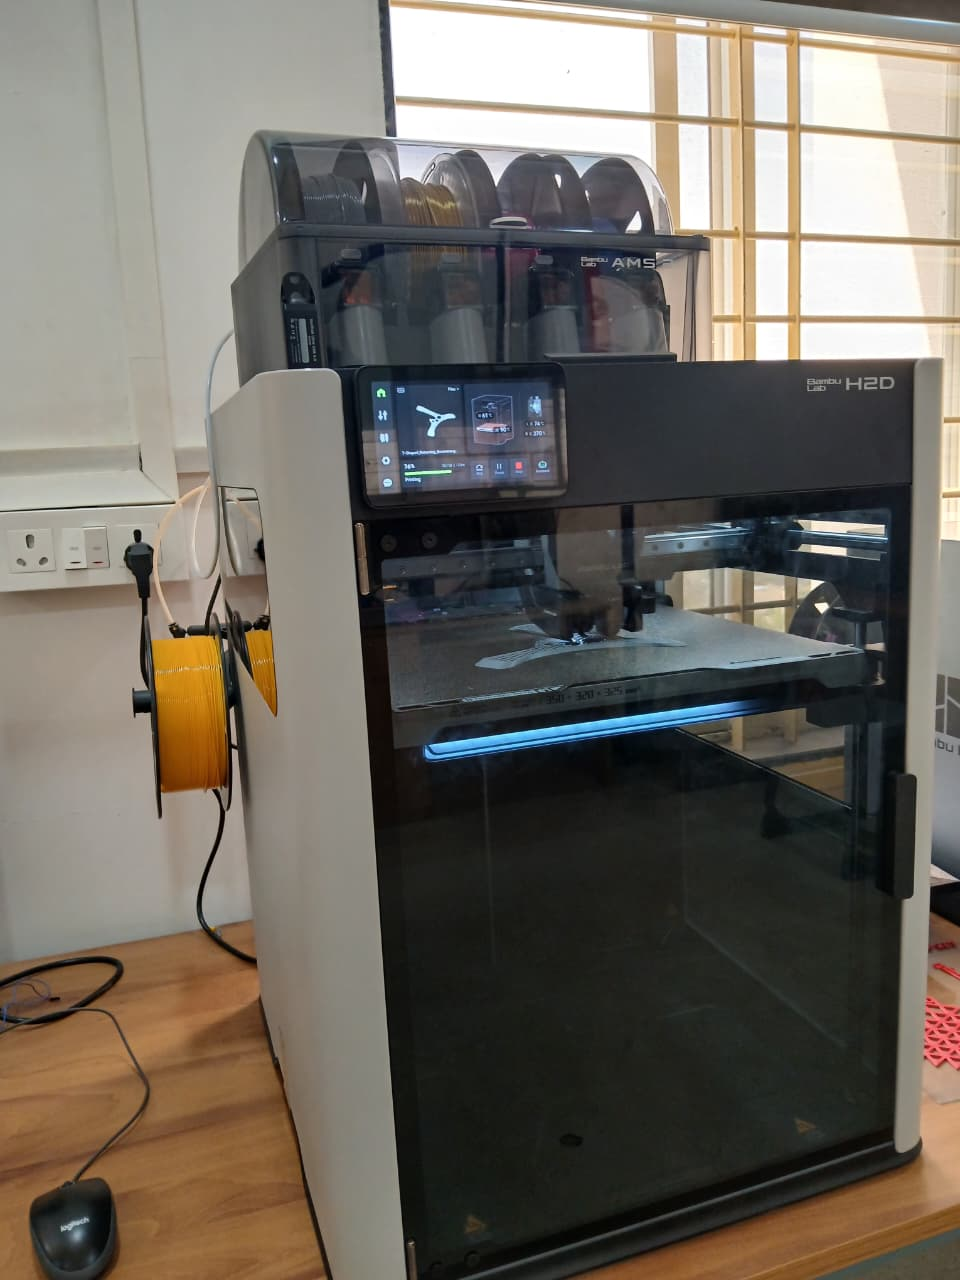
\includegraphics[height=40mm,width=\linewidth,keepaspectratio]{3DP_Bambu_H2D_With_AMS.jpeg}\caption{Bambu Lab H2D with AMS}\end{subfigure}\hfill
\begin{subfigure}[b]{0.24\linewidth}\centering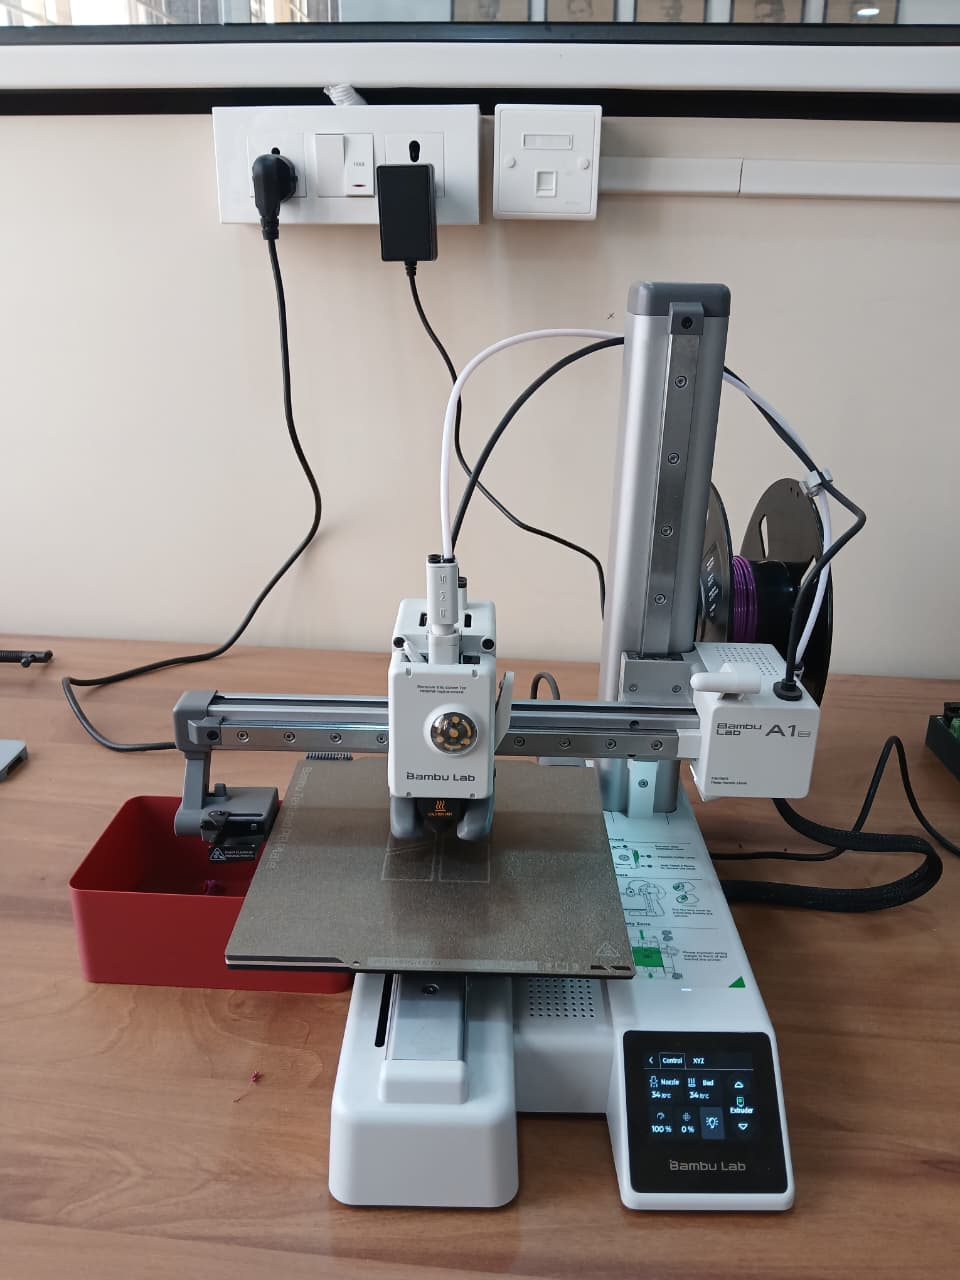
\includegraphics[height=40mm,width=\linewidth,keepaspectratio]{3DP_Bambu_A1_Mini.jpeg}\caption{Bambu Lab A1 mini}\end{subfigure}\hfill
\begin{subfigure}[b]{0.24\linewidth}\centering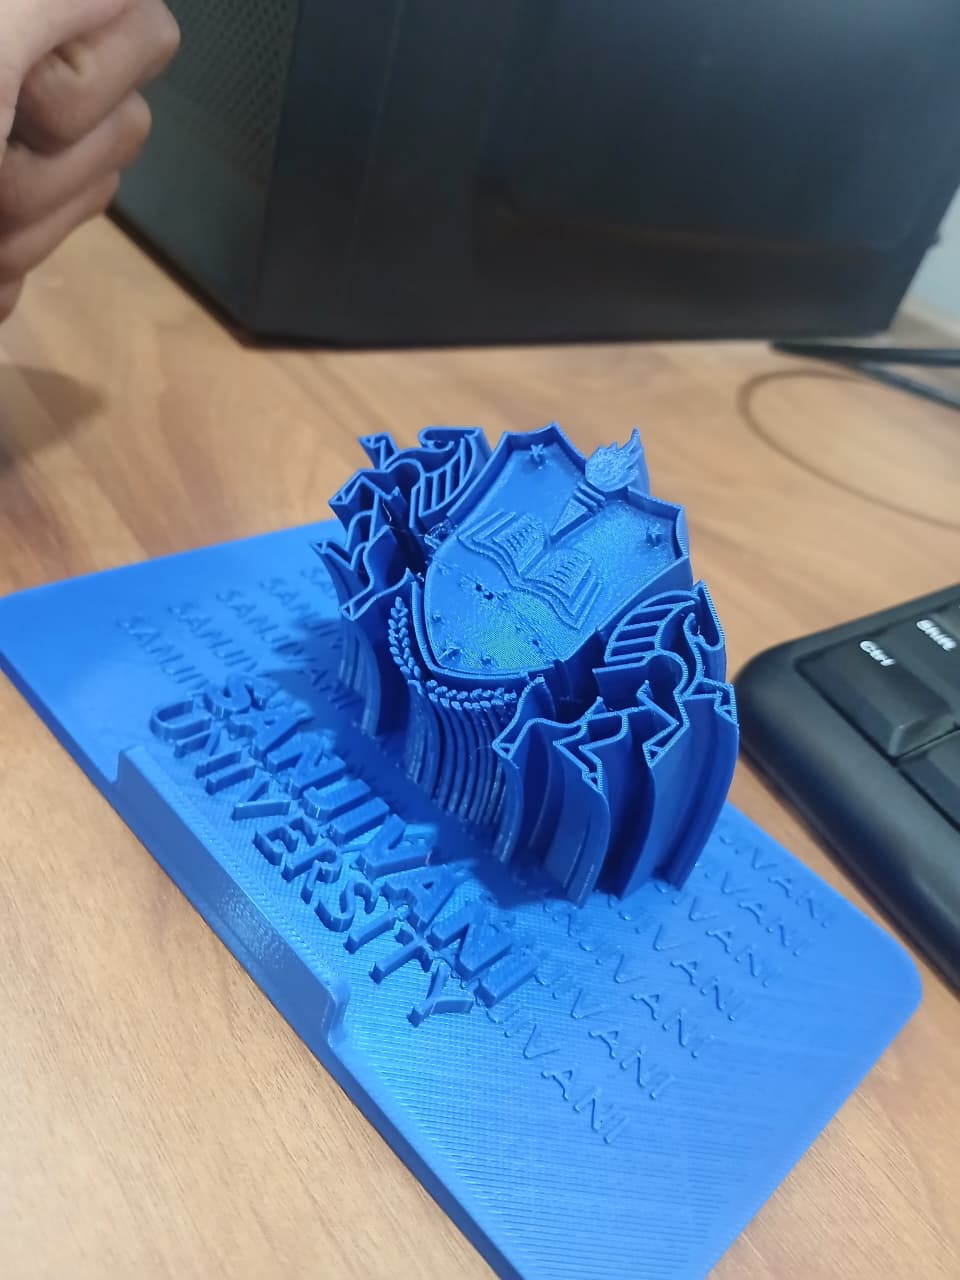
\includegraphics[height=40mm,width=\linewidth,keepaspectratio]{3DP_Phone Stand Sanjivani University.jpeg}\caption{Phone stand, Sanjivani University}\end{subfigure}\hfill
\begin{subfigure}[b]{0.24\linewidth}\centering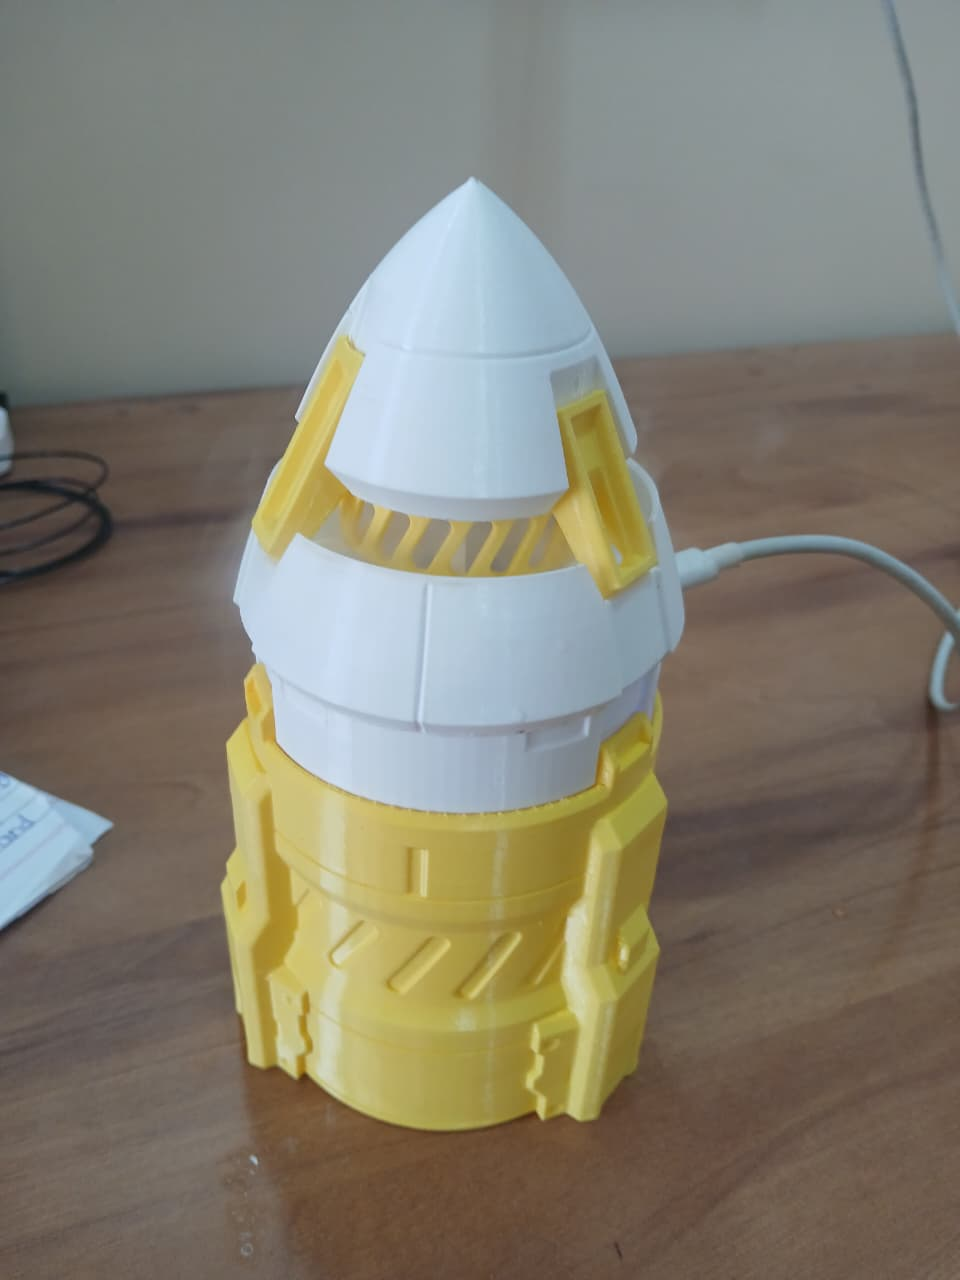
\includegraphics[height=40mm,width=\linewidth,keepaspectratio]{3DP_Humidifier.jpeg}\caption{Humidifier}\end{subfigure}
\caption{Our own photographs from Tinkerers' Lab (captions are the photos' file names).}
\label{fig:digifab}
\end{figure}

\section{Laser cutting (CO$_2$)}
A CO$_2$ laser focuses an infrared beam onto a sheet to burn a line through it (cutting) or mark its surface (engraving).
\textbf{Workflow:} 2D design as DXF or SVG $\rightarrow$ laser software (power, speed and job per colour) $\rightarrow$ material setup (allowed sheet, flat on the honeycomb) $\rightarrow$ focus (beam narrowest at the surface) $\rightarrow$ cut or engrave with extraction and air assist on, after a test on scrap $\rightarrow$ inspect cut-through, fit and kerf.

\subsection{How the laser head moves}
The laser tube stays fixed at the back of the machine; only mirrors move (Figure~\ref{fig:lasermotion}). The \textcolor{cbclay}{\textbf{head travels left--right along the gantry (X)}} and the \textcolor{cbwater}{\textbf{gantry travels front--back on two rails (Y)}}. The beam goes from the tube to mirror~1 (fixed), along the Y rail to mirror~2 (on the gantry), along the gantry to mirror~3 in the head, and down through the focusing lens to a point on the sheet. Because the beam path changes length as the head moves, the three mirrors must be aligned so the beam reaches the lens centre anywhere on the bed.

\begin{figure}[H]
\centering
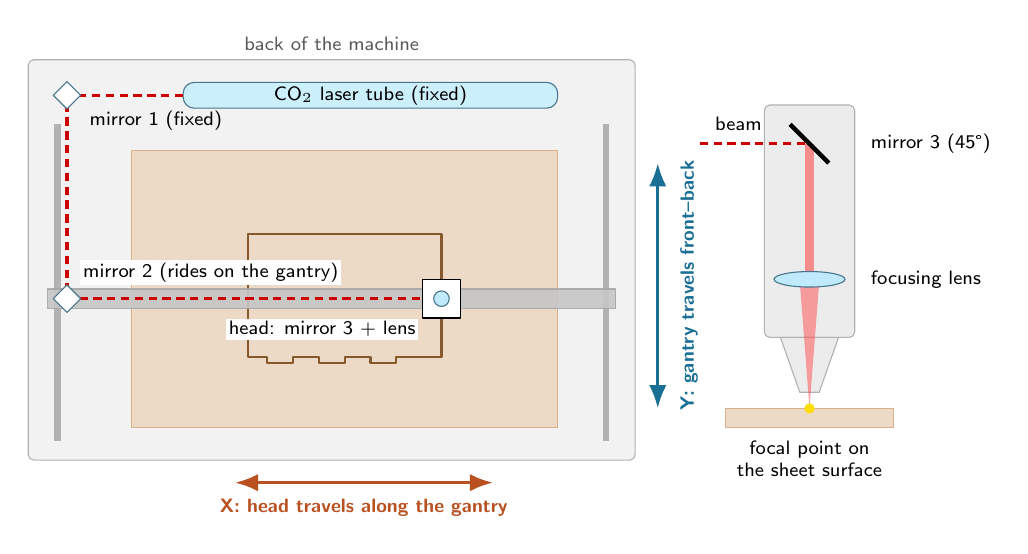
\begin{tikzpicture}[scale=0.82, font=\sffamily\scriptsize, line join=round]
  \draw[fill=gray!10, draw=gray!60, rounded corners=2pt] (0,0) rectangle (9.4,6.2);
  \node[gray!70!black] at (4.7,6.45) {back of the machine};
  \draw[fill=brown!30, draw=brown!60] (1.6,0.5) rectangle (8.2,4.8);
  \draw[brown!70!black, thick] (3.4,1.6) -- (3.7,1.6) -- (3.7,1.5) -- (4.1,1.5) -- (4.1,1.6) -- (4.5,1.6) -- (4.5,1.5) -- (4.9,1.5) -- (4.9,1.6) -- (5.3,1.6) -- (5.3,1.5) -- (5.7,1.5) -- (5.7,1.6) -- (6.4,1.6) -- (6.4,3.5) -- (3.4,3.5) -- cycle;
  \draw[line width=2.4pt, gray!60] (0.45,0.3) -- (0.45,5.2) (8.95,0.3) -- (8.95,5.2);
  \draw[fill=cyan!20, draw=cyan!50!black, rounded corners=4pt] (2.4,5.45) rectangle (8.2,5.85);
  \node at (5.3,5.65) {CO$_2$ laser tube (fixed)};
  \draw[fill=gray!45, draw=gray!70, opacity=0.9] (0.3,2.35) rectangle (9.1,2.65);
  \draw[red!80!black, very thick, densely dashed] (2.4,5.65) -- (0.6,5.65) -- (0.6,2.5) -- (6.4,2.5);
  \draw[fill=white, draw=cyan!50!black, rotate around={45:(0.6,5.65)}] (0.45,5.5) rectangle (0.75,5.8);
  \draw[fill=white, draw=cyan!50!black, rotate around={45:(0.6,2.5)}] (0.45,2.35) rectangle (0.75,2.65);
  \draw[fill=white, draw=black] (6.1,2.2) rectangle (6.7,2.8);
  \draw[fill=cyan!25, draw=cyan!50!black] (6.4,2.5) circle (0.12);
  \node[anchor=west] at (0.8,5.25) {mirror 1 (fixed)};
  \node[anchor=south west, fill=white, inner sep=1pt] at (0.8,2.7) {mirror 2 (rides on the gantry)};
  \node[anchor=north east, fill=white, inner sep=1pt] at (6.05,2.2) {head: mirror 3 + lens};
  \draw[{Latex}-{Latex}, cbclay, very thick] (3.2,-0.35) -- (7.2,-0.35);
  \node[cbclay, anchor=north] at (5.2,-0.45) {\textbf{X: head travels along the gantry}};
  \draw[{Latex}-{Latex}, cbwater, very thick] (9.75,0.8) -- (9.75,4.6);
  \node[cbwater, rotate=90, anchor=north] at (9.95,2.7) {\textbf{Y: gantry travels front--back}};
  % side cut-away of the head
  \begin{scope}[shift={(11.4,0.3)}]
    \draw[fill=gray!15, draw=gray!60, rounded corners=2pt] (0,1.6) rectangle (1.4,5.2);
    \draw[fill=gray!15, draw=gray!60] (0.25,1.6) -- (1.15,1.6) -- (0.85,0.75) -- (0.55,0.75) -- cycle;
    \draw[red!80!black, very thick, densely dashed] (-1.0,4.6) -- (0.7,4.6);
    \draw[red!70, line width=3pt, opacity=0.6] (0.7,4.6) -- (0.7,2.55);
    \fill[red!70, opacity=0.5] (0.55,2.45) -- (0.85,2.45) -- (0.7,0.5) -- cycle;
    \draw[black, line width=1.6pt] (0.4,4.9) -- (1.0,4.3);
    \draw[fill=cyan!25, draw=cyan!50!black] (0.7,2.5) ellipse (0.55 and 0.12);
    \draw[fill=brown!30, draw=brown!60] (-0.6,0.2) rectangle (2.0,0.5);
    \fill[yellow!80!orange] (0.7,0.5) circle (0.08);
    \node[anchor=west] at (1.5,4.6) {mirror 3 (45\textdegree)};
    \node[anchor=west] at (1.5,2.5) {focusing lens};
    \node[anchor=north, align=center] at (0.7,0.15) {focal point on\\the sheet surface};
    \node[anchor=south] at (-0.4,4.65) {beam};
  \end{scope}
\end{tikzpicture}
\caption{How the laser head moves: top view (left) and side cut-away of the head (right). The head traces one side panel of our enclosure.}
\label{fig:lasermotion}
\end{figure}

\subsection{Unidirectional vs bidirectional engraving}
A raster engraving is built from many parallel lines (Figure~\ref{fig:scan}).
\textbf{Unidirectional} engraving fires in one direction only and returns without firing, so every line starts from the same side: slower (about twice the passes) but with clean edges.
\textbf{Bidirectional} engraving fires on both passes and takes about half the time, but lines engraved in opposite directions only line up if the \emph{scan offset} (scan-gap) is calibrated; otherwise edges look doubled or jagged.

\begin{figure}[H]
\centering
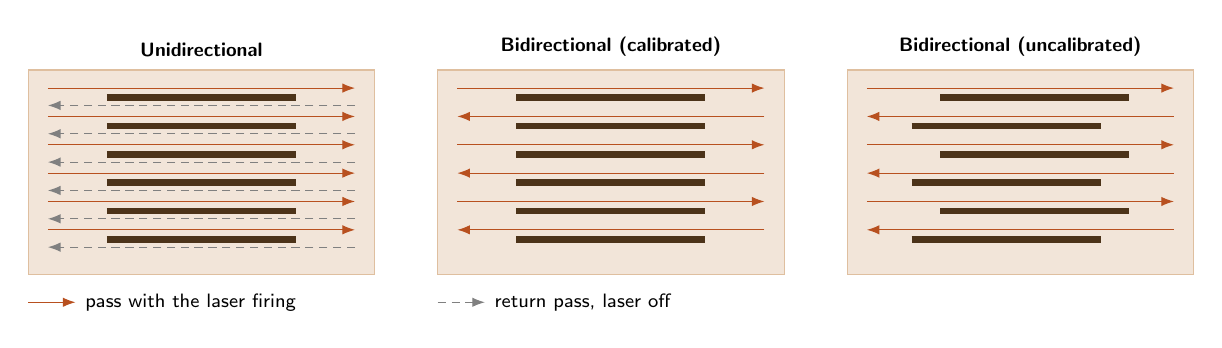
\begin{tikzpicture}[font=\sffamily\scriptsize, >={Latex[length=1.6mm]}]
  \foreach \px/\ttl/\md in {0/Unidirectional/uni, 5.2/Bidirectional (calibrated)/bi, 10.4/Bidirectional (uncalibrated)/bad} {
    \begin{scope}[shift={(\px,0)}]
      \draw[fill=brown!20, draw=brown!50] (0,0) rectangle (4.4,2.6);
      \node[anchor=south] at (2.2,2.65) {\textbf{\ttl}};
      \foreach \i in {0,...,5} {
        \pgfmathsetmacro{\y}{2.25-\i*0.36}
        \pgfmathsetmacro{\sh}{0}
        \ifnum\i=1 \def\odd{1}\else\ifnum\i=3 \def\odd{1}\else\ifnum\i=5 \def\odd{1}\else\def\odd{0}\fi\fi\fi
        \def\uni{uni}\def\bad{bad}
        \ifx\md\uni
          \draw[brown!40!black, line width=2.4pt] (1.0,\y) -- (3.4,\y);
          \draw[->, cbclay, thin] (0.25,\y+0.12) -- (4.15,\y+0.12);
          \draw[->, gray, thin, densely dashed] (4.15,\y-0.1) -- (0.25,\y-0.1);
        \else
          \ifx\md\bad
            \ifnum\odd=1 \pgfmathsetmacro{\sh}{-0.18}\else\pgfmathsetmacro{\sh}{0.18}\fi
          \fi
          \draw[brown!40!black, line width=2.4pt] (1.0+\sh,\y) -- (3.4+\sh,\y);
          \ifnum\odd=1
            \draw[->, cbclay, thin] (4.15,\y+0.12) -- (0.25,\y+0.12);
          \else
            \draw[->, cbclay, thin] (0.25,\y+0.12) -- (4.15,\y+0.12);
          \fi
        \fi
      }
    \end{scope}
  }
  \draw[->, cbclay, thin] (0,-0.35) -- (0.6,-0.35) node[right, black] {pass with the laser firing};
  \draw[->, gray, thin, densely dashed] (5.2,-0.35) -- (5.8,-0.35) node[right, black] {return pass, laser off};
\end{tikzpicture}
\caption{Raster engraving. Unidirectional: clean edges, empty return passes. Bidirectional: half the passes; without scan-offset calibration, alternate lines shift and the edges become jagged.}
\label{fig:scan}
\end{figure}

\begin{table}[H]
\centering\small
\caption{Laser settings, one line each.}
\begin{tabularx}{\linewidth}{@{}>{\bfseries\raggedright\arraybackslash}p{0.22\linewidth}X@{}}
\toprule
Setting & \textbf{What it does} \\
\midrule
Power \%, speed & Share of the tube's output and head speed; tuned together on a test grid for each material. \\
Frequency / PPI & How often the laser pulses (pulses per inch); lower tends to char wood less, higher gives smoother acrylic edges. \\
Focus / focal length & The distance at which the beam is narrowest; the sheet surface must sit there. \\
Kerf & The width of material the beam burns away; half comes off each side of the line, so tabs shrink and slots grow. \\
Kerf compensation & Offsetting paths by half the measured kerf so press-fit parts come out at size. \\
Vector vs raster & A vector cut follows a line through the sheet; a raster engrave sweeps line by line to burn an image into the surface. \\
Uni- / bidirectional & Raster firing on one pass direction only, or on both; bidirectional needs scan-offset calibration. \\
Air assist, passes & An air jet clears smoke and flame and protects the lens; two gentle passes can char less than one slow pass. \\
\bottomrule
\end{tabularx}
\end{table}

\noindent\textbf{Allowed:} MDF (medium-density fibreboard), plywood, acrylic, cardboard, paper. \textbf{Never cut:} PVC or vinyl (chlorine gas), polycarbonate (burns and discolours), coated metals (not cut by CO$_2$; coatings reflect or fume), or any unidentified sheet.

\noindent\textbf{Lab machine:} SIL CO$_2$ laser cutter, 100\,W. Bed size and other specifications: [to confirm from machine label].

\section{Applied in ClayBreeze: electronics enclosure}
\label{sec:enclosure}
The laser-cutting practice is being put to work on the project: a finger-jointed box to house the ESP32, the relay module and the DHT11 wiring. \textbf{Status: laser cutting in progress.} The cutting file is \texttt{cad/dxf-enclosure/basic-box-120x150x100-3mm.dxf} in the GitHub repository. Read with \texttt{ezdxf}, it holds \textbf{six closed, finger-jointed panels} (432 line segments, millimetres) nested on a 426 $\times$ 253\,mm area, for a 120 $\times$ 150 $\times$ 100\,mm box (Table~\ref{tab:enclosure}, Figure~\ref{fig:enclosure}). Material: 3\,mm MDF, as stated in the file names. Which panel is the top, and the cable and sensor cut-outs, are not yet decided.

\begin{table}[H]
\centering\small
\caption{Panels in the enclosure DXF (outer bounding size; named by size only).}
\label{tab:enclosure}
\begin{tabular}{@{}lcc@{}}
\toprule
Panels & Size (mm) & Qty \\
\midrule
Top and bottom & 120 $\times$ 150 & 2 \\
Long sides & 150 $\times$ 100 & 2 \\
Short sides & 120 $\times$ 100 & 2 \\
\bottomrule
\end{tabular}
\end{table}

\begin{figure}[H]
\centering
\begin{subfigure}[b]{0.52\linewidth}\centering
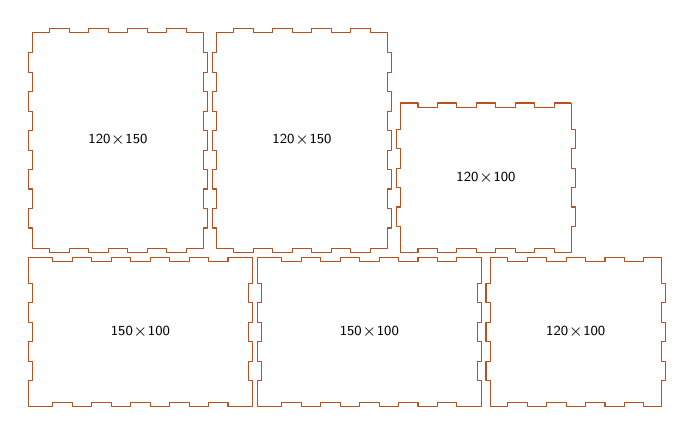
\begin{tikzpicture}[x=0.19mm, y=0.19mm, font=\sffamily\tiny]
% Generated from cad/dxf-enclosure/basic-box-120x150x100-3mm.dxf (432 LINE entities, mm).
% Do not edit by hand; regenerate from the DXF.
\draw[cbclay, line width=0.4pt, line join=round] (423,100) -- (411.5,100) -- (411.5,97) -- (398.5,97) -- (398.5,100) -- (385.5,100) -- (385.5,97) -- (372.5,97) -- (372.5,100) -- (359.5,100) -- (359.5,97) -- (346.5,97) -- (346.5,100) -- (333.5,100) -- (333.5,97) -- (320.5,97) -- (320.5,100) -- (309,100) -- (309,97) -- (309,82.5) -- (306,82.5) -- (306,69.5) -- (309,69.5) -- (309,56.5) -- (306,56.5) -- (306,43.5) -- (309,43.5) -- (309,30.5) -- (306,30.5) -- (306,17.5) -- (309,17.5) -- (309,3) -- (309,0) -- (320.5,0) -- (320.5,3) -- (333.5,3) -- (333.5,0) -- (346.5,0) -- (346.5,3) -- (359.5,3) -- (359.5,0) -- (372.5,0) -- (372.5,3) -- (385.5,3) -- (385.5,0) -- (398.5,0) -- (398.5,3) -- (411.5,3) -- (411.5,0) -- (423,0) -- (423,3) -- (423,17.5) -- (426,17.5) -- (426,30.5) -- (423,30.5) -- (423,43.5) -- (426,43.5) -- (426,56.5) -- (423,56.5) -- (423,69.5) -- (426,69.5) -- (426,82.5) -- (423,82.5) -- (423,97) -- (423,100)
(363,203) -- (351.5,203) -- (351.5,200) -- (338.5,200) -- (338.5,203) -- (325.5,203) -- (325.5,200) -- (312.5,200) -- (312.5,203) -- (299.5,203) -- (299.5,200) -- (286.5,200) -- (286.5,203) -- (273.5,203) -- (273.5,200) -- (260.5,200) -- (260.5,203) -- (249,203) -- (249,200) -- (249,185.5) -- (246,185.5) -- (246,172.5) -- (249,172.5) -- (249,159.5) -- (246,159.5) -- (246,146.5) -- (249,146.5) -- (249,133.5) -- (246,133.5) -- (246,120.5) -- (249,120.5) -- (249,106) -- (249,103) -- (260.5,103) -- (260.5,106) -- (273.5,106) -- (273.5,103) -- (286.5,103) -- (286.5,106) -- (299.5,106) -- (299.5,103) -- (312.5,103) -- (312.5,106) -- (325.5,106) -- (325.5,103) -- (338.5,103) -- (338.5,106) -- (351.5,106) -- (351.5,103) -- (363,103) -- (363,106) -- (363,120.5) -- (366,120.5) -- (366,133.5) -- (363,133.5) -- (363,146.5) -- (366,146.5) -- (366,159.5) -- (363,159.5) -- (363,172.5) -- (366,172.5) -- (366,185.5) -- (363,185.5) -- (363,200) -- (363,203)
(150,100) -- (147,100) -- (133.5,100) -- (133.5,97) -- (120.5,97) -- (120.5,100) -- (107.5,100) -- (107.5,97) -- (94.5,97) -- (94.5,100) -- (81.5,100) -- (81.5,97) -- (68.5,97) -- (68.5,100) -- (55.5,100) -- (55.5,97) -- (42.5,97) -- (42.5,100) -- (29.5,100) -- (29.5,97) -- (16.5,97) -- (16.5,100) -- (3,100) -- (0,100) -- (0,97) -- (0,82.5) -- (3,82.5) -- (3,69.5) -- (0,69.5) -- (0,56.5) -- (3,56.5) -- (3,43.5) -- (0,43.5) -- (0,30.5) -- (3,30.5) -- (3,17.5) -- (0,17.5) -- (0,3) -- (0,0) -- (3,0) -- (16.5,0) -- (16.5,3) -- (29.5,3) -- (29.5,0) -- (42.5,0) -- (42.5,3) -- (55.5,3) -- (55.5,0) -- (68.5,0) -- (68.5,3) -- (81.5,3) -- (81.5,0) -- (94.5,0) -- (94.5,3) -- (107.5,3) -- (107.5,0) -- (120.5,0) -- (120.5,3) -- (133.5,3) -- (133.5,0) -- (147,0) -- (150,0) -- (150,3) -- (150,17.5) -- (147,17.5) -- (147,30.5) -- (150,30.5) -- (150,43.5) -- (147,43.5) -- (147,56.5) -- (150,56.5) -- (150,69.5) -- (147,69.5) -- (147,82.5) -- (150,82.5) -- (150,97) -- (150,100)
(303,100) -- (300,100) -- (286.5,100) -- (286.5,97) -- (273.5,97) -- (273.5,100) -- (260.5,100) -- (260.5,97) -- (247.5,97) -- (247.5,100) -- (234.5,100) -- (234.5,97) -- (221.5,97) -- (221.5,100) -- (208.5,100) -- (208.5,97) -- (195.5,97) -- (195.5,100) -- (182.5,100) -- (182.5,97) -- (169.5,97) -- (169.5,100) -- (156,100) -- (153,100) -- (153,97) -- (153,82.5) -- (156,82.5) -- (156,69.5) -- (153,69.5) -- (153,56.5) -- (156,56.5) -- (156,43.5) -- (153,43.5) -- (153,30.5) -- (156,30.5) -- (156,17.5) -- (153,17.5) -- (153,3) -- (153,0) -- (156,0) -- (169.5,0) -- (169.5,3) -- (182.5,3) -- (182.5,0) -- (195.5,0) -- (195.5,3) -- (208.5,3) -- (208.5,0) -- (221.5,0) -- (221.5,3) -- (234.5,3) -- (234.5,0) -- (247.5,0) -- (247.5,3) -- (260.5,3) -- (260.5,0) -- (273.5,0) -- (273.5,3) -- (286.5,3) -- (286.5,0) -- (300,0) -- (303,0) -- (303,3) -- (303,17.5) -- (300,17.5) -- (300,30.5) -- (303,30.5) -- (303,43.5) -- (300,43.5) -- (300,56.5) -- (303,56.5) -- (303,69.5) -- (300,69.5) -- (300,82.5) -- (303,82.5) -- (303,97) -- (303,100)
(105.5,253) -- (92.5,253) -- (92.5,250) -- (79.5,250) -- (79.5,253) -- (66.5,253) -- (66.5,250) -- (53.5,250) -- (53.5,253) -- (40.5,253) -- (40.5,250) -- (27.5,250) -- (27.5,253) -- (14.5,253) -- (14.5,250) -- (3,250) -- (3,236.5) -- (0,236.5) -- (0,223.5) -- (3,223.5) -- (3,210.5) -- (0,210.5) -- (0,197.5) -- (3,197.5) -- (3,184.5) -- (0,184.5) -- (0,171.5) -- (3,171.5) -- (3,158.5) -- (0,158.5) -- (0,145.5) -- (3,145.5) -- (3,132.5) -- (0,132.5) -- (0,119.5) -- (3,119.5) -- (3,106) -- (14.5,106) -- (14.5,103) -- (27.5,103) -- (27.5,106) -- (40.5,106) -- (40.5,103) -- (53.5,103) -- (53.5,106) -- (66.5,106) -- (66.5,103) -- (79.5,103) -- (79.5,106) -- (92.5,106) -- (92.5,103) -- (105.5,103) -- (105.5,106) -- (117,106) -- (117,119.5) -- (120,119.5) -- (120,132.5) -- (117,132.5) -- (117,145.5) -- (120,145.5) -- (120,158.5) -- (117,158.5) -- (117,171.5) -- (120,171.5) -- (120,184.5) -- (117,184.5) -- (117,197.5) -- (120,197.5) -- (120,210.5) -- (117,210.5) -- (117,223.5) -- (120,223.5) -- (120,236.5) -- (117,236.5) -- (117,250) -- (105.5,250) -- (105.5,253)
(228.5,253) -- (215.5,253) -- (215.5,250) -- (202.5,250) -- (202.5,253) -- (189.5,253) -- (189.5,250) -- (176.5,250) -- (176.5,253) -- (163.5,253) -- (163.5,250) -- (150.5,250) -- (150.5,253) -- (137.5,253) -- (137.5,250) -- (126,250) -- (126,236.5) -- (123,236.5) -- (123,223.5) -- (126,223.5) -- (126,210.5) -- (123,210.5) -- (123,197.5) -- (126,197.5) -- (126,184.5) -- (123,184.5) -- (123,171.5) -- (126,171.5) -- (126,158.5) -- (123,158.5) -- (123,145.5) -- (126,145.5) -- (126,132.5) -- (123,132.5) -- (123,119.5) -- (126,119.5) -- (126,106) -- (137.5,106) -- (137.5,103) -- (150.5,103) -- (150.5,106) -- (163.5,106) -- (163.5,103) -- (176.5,103) -- (176.5,106) -- (189.5,106) -- (189.5,103) -- (202.5,103) -- (202.5,106) -- (215.5,106) -- (215.5,103) -- (228.5,103) -- (228.5,106) -- (240,106) -- (240,119.5) -- (243,119.5) -- (243,132.5) -- (240,132.5) -- (240,145.5) -- (243,145.5) -- (243,158.5) -- (240,158.5) -- (240,171.5) -- (243,171.5) -- (243,184.5) -- (240,184.5) -- (240,197.5) -- (243,197.5) -- (243,210.5) -- (240,210.5) -- (240,223.5) -- (243,223.5) -- (243,236.5) -- (240,236.5) -- (240,250) -- (228.5,250) -- (228.5,253);

\node at (60,178) {120$\times$150}; \node at (183,178) {120$\times$150}; \node at (306,153) {120$\times$100};
\node at (75,50) {150$\times$100}; \node at (228,50) {150$\times$100}; \node at (366,50) {120$\times$100};
\end{tikzpicture}
\caption{The DXF, drawn from its own line data.}
\end{subfigure}\hfill
\begin{subfigure}[b]{0.44\linewidth}\centering
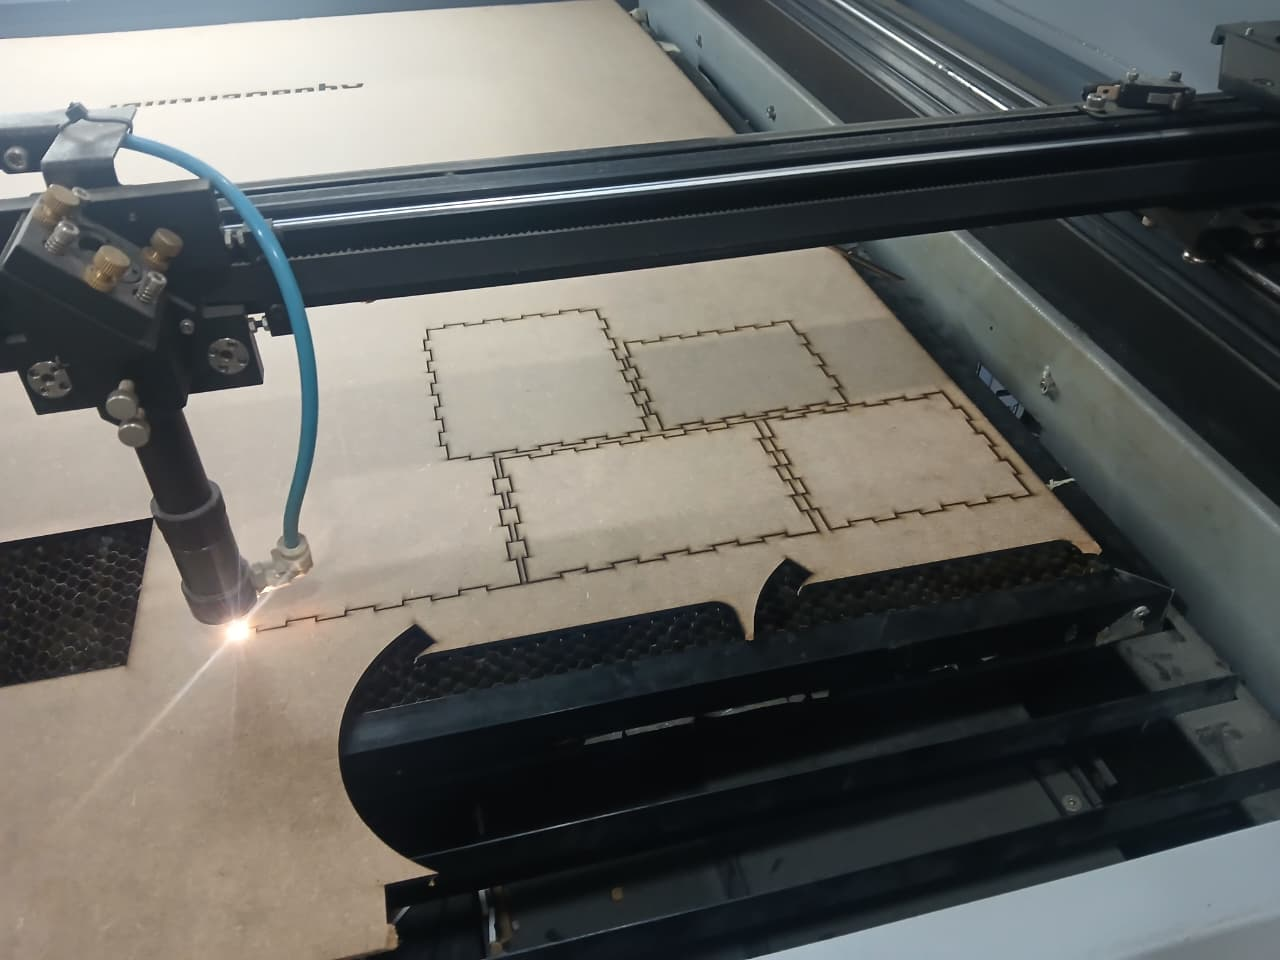
\includegraphics[width=\linewidth]{enclosure-cutting.jpg}
\caption{Laser cutting MDF to store electronics.}
\end{subfigure}
\caption{ClayBreeze electronics enclosure: six finger-jointed panels in 3\,mm MDF (laser cutting in progress).}
\label{fig:enclosure}
\end{figure}

\section{Safety checklist}
\begin{itemize}
\item Fume extraction and ventilation on; ABS/ASA only in an enclosed printer in a ventilated room.
\item Only allowed sheets on the laser; never leave the laser unattended while it runs.
\item Fire-watch: bed clear of offcuts, extinguisher location known, stop the job if a flame does not go out.
\item PPE (personal protective equipment): the closed lid is the beam shield; safety glasses and gloves for sanding, support removal and sharp offcuts.
\item Hot parts: nozzles reach 300--350\degC{} and beds up to 120\degC; let them cool before touching.
\end{itemize}

% ======================= REFERENCES =======================
\begin{thebibliography}{99}
\addcontentsline{toc}{chapter}{References}
\bibitem{icap} Ministry of Environment, Forest \& Climate Change (Ozone Cell), Government of India. \emph{India Cooling Action Plan}. New Delhi, March 2019. \url{https://ozonecell.nic.in/india-cooling-action-plan}
\bibitem{watson} J.\,A.~Watson, C.~G\'omez, R.~Bucklin, J.\,D.~Leary, D.\,B.~McConnell. \emph{Fan and Pad Greenhouse Evaporative Cooling Systems}. University of Florida IFAS Extension, CIR1135/AE069. \url{https://edis.ifas.ufl.edu/AE069}
\bibitem{laknizi} A.~Laknizi, A.~Ben Abdellah, M.~Faqir, E.~Essadiqi, S.~Dhimdi. Performance characterization of a direct evaporative cooling pad based on pottery material. \emph{International Journal of Sustainable Engineering}, 14(1):46--56, 2021. doi:10.1080/19397038.2019.1677800
\bibitem{mittal} A.~Mittal, T.~Kataria, G.\,K.~Das, S.\,G.~Chatterjee. Evaporative cooling of water in a small vessel under varying ambient humidity. \emph{International Journal of Green Energy}, 3(4):347--368, 2006. doi:10.1080/01971520600704654
\bibitem{hoyano} J.~He, A.~Hoyano. Experimental study of cooling effects of a passive evaporative cooling wall constructed of porous ceramics with high water soaking-up ability. \emph{Building and Environment}, 45(2):461--472, 2010. doi:10.1016/j.buildenv.2009.07.002
\bibitem{elsaid} E.\,M.\,S.~El-Said et al. Experimental investigation of earth-air heat exchanger using porous clay vessels for eco-friendly buildings. \emph{Scientific Reports}, 14:17548, 2024. \url{https://www.nature.com/articles/s41598-024-67212-5}
\bibitem{jain} J.\,K.~Jain, D.\,A.~Hindoliya. Experimental performance of new evaporative cooling pad materials. \emph{Sustainable Cities and Society}, 1(4):252--256, 2011. doi:10.1016/j.scs.2011.07.005
\bibitem{alsulaiman} F.~Al-Sulaiman. Evaluation of the performance of local fibers in evaporative cooling. \emph{Energy Conversion and Management}, 43(16):2267--2273, 2002. doi:10.1016/S0196-8904(01)00121-2
\bibitem{doe} U.S. Department of Energy, Federal Energy Management Program. \emph{Best Management Practice \#13: Other Water-Intensive Processes}. \url{https://www.energy.gov/cmei/femp/best-management-practice-13-other-water-intensive-processes}
\bibitem{epa} U.S. Environmental Protection Agency. \emph{Transitioning to Low-GWP Alternatives in Residential and Light Commercial Air Conditioning}. \url{https://www.epa.gov/snap/transitioning-low-gwp-alternatives-residential-and-light-commercial-air-conditioning}
\bibitem{energystar} ENERGY STAR. \emph{Room Air Conditioners}. \url{https://www.energystar.gov/products/room_air_conditioners}
\bibitem{toi} The Times of India / ETimes Trending Desk. Inside Project Vayu: Delhi students turn kulhads and scrap wood into eco-coolers for underprivileged government school kids. 8 May 2026. (Inspiration only.)
\bibitem{wakchaure} K.~Wakchaure. Fab Academy documentation (2022), Vigyan Ashram: about page, Week~3 (computer-controlled cutting) and Week~5 (3D scanning and printing). \url{https://fabacademy.org/2022/labs/vigyanashram/students/kiran-wakchaure/about.html} (learning reference; paraphrased)
\bibitem{bambuh2d} Bambu Lab. H2D technical specifications and product page. \url{https://bambulab.com/en/h2d/tech-specs}, \url{https://bambulab.com/en/h2d} (accessed 26 Nov 2026)
\bibitem{bambup1s} Bambu Lab. P1S product page, parameters comparison; P1 series page (CoreXY). \url{https://us.store.bambulab.com/products/p1s}, \url{https://bambulab.com/en/p1} (accessed 26 Nov 2026)
\bibitem{bambua1} Bambu Lab. A1 technical specifications and product page (``bed slinger''). \url{https://bambulab.com/en/a1/tech-specs}, \url{https://bambulab.com/en/a1} (accessed 26--27 Nov 2026)
\bibitem{bambua1mini} Bambu Lab. A1 mini technical specifications and product page (``bed slinger''). \url{https://bambulab.com/en/a1-mini/tech-specs}, \url{https://bambulab.com/en/a1-mini} (accessed 26--27 Nov 2026)
\bibitem{bambuh2dwiki} Bambu Lab Wiki. Introduction to H2D --- Core XY movement system. \url{https://wiki.bambulab.com/en/h2/manual/h2d-intro} (accessed 27 Nov 2026)
\bibitem{bambuwiki} Bambu Lab Wiki. Filament guide --- printer, nozzle, AMS, build plate, glue compatibility and required parameters. \url{https://wiki.bambulab.com/en/general/filament-guide-material-table} (accessed 26 Nov 2026)
\bibitem{bambuimages} Bambu Lab. Official product images of the H2D, P1S, A1 and A1 mini, from the official store pages \url{https://us.store.bambulab.com/products/h2d}, \url{https://us.store.bambulab.com/products/p1s}, \url{https://us.store.bambulab.com/products/a1}, \url{https://us.store.bambulab.com/products/a1-mini}. Images \textcopyright\ Bambu Lab (accessed 26 Nov 2026)
\bibitem{afn} Action For Nature. 2026 International Young Eco-Hero Award listing describing Project Vaayu. \url{https://actionfornature.org/eco-hero-winners/tag/Terracotta%2BCooling}
\end{thebibliography}

\end{document}
